\documentclass[a4paper, 11pt]{report}

% basics
\usepackage[utf8]{inputenc}
\usepackage[T1]{fontenc}
\usepackage{textcomp}
% \usepackage[dutch]{babel}
\usepackage{url}
\usepackage{hyperref}
\hypersetup{
    colorlinks,
    linkcolor={black},
    citecolor={black},
    urlcolor={blue!80!black},
    % backref=true, 
    % pagebackref=true
}
% Page Margins
\usepackage[
    margin=2.5cm, 
    % top=2.8cm, bottom=2.8cm,
    % left=1in, right=1in, 
    % headheight=14.5pt
    ]{geometry}

\usepackage{setspace}
\setstretch{1.15}

\usepackage{graphicx}
\usepackage{float}
\usepackage{booktabs}
\usepackage{pdfpages}
\usepackage[shortlabels]{enumitem}
% \usepackage{parskip}
\usepackage{emptypage}
\usepackage{subcaption}
\usepackage{multicol}
\usepackage[usenames,dvipsnames]{xcolor}

% \usepackage{cmbright}

\usepackage{amsmath, amsfonts, mathtools, amsthm, amssymb}
\usepackage{mathrsfs}
% \usepackage{dutchcal} % \mathcal: also small letters. \mathbcal = bold ones. % https://tex.stackexchange.com/a/641540/114006
\usepackage{braket} % https://tex.stackexchange.com/a/253232/114006
\usepackage{cancel}
\usepackage{bm}
\usepackage[ruled,vlined,linesnumbered]{algorithm2e} % SeniorMars template
% \usepackage{lipsum}
\usepackage{pgfplots}
\usepgfplotslibrary{fillbetween}

\newcommand\N{\ensuremath{\mathbb{N}}}
\newcommand\R{\ensuremath{\mathbb{R}}}
\newcommand\Z{\ensuremath{\mathbb{Z}}}
\renewcommand\O{\ensuremath{\emptyset}}
\newcommand\Q{\ensuremath{\mathbb{Q}}}
\newcommand\C{\ensuremath{\mathbb{C}}}
\DeclareMathOperator{\sgn}{sgn}
\usepackage{systeme}
\let\svlim\lim\def\lim{\svlim\limits}
\let\implies\Rightarrow
\let\impliedby\Leftarrow
\let\iff\Leftrightarrow
\let\epsilon\varepsilon
\usepackage{stmaryrd} % for \lightning
\newcommand\contra{\scalebox{1.1}{$\lightning$}}
% \let\phi\varphi





% correct
\definecolor{correct}{HTML}{009900}
\newcommand\correct[2]{\ensuremath{\:}{\color{red}{#1}}\ensuremath{\to }{\color{correct}{#2}}\ensuremath{\:}}
\newcommand\green[1]{{\color{correct}{#1}}}



% horizontal rule
\newcommand\hr{
    \noindent\rule[0.5ex]{\linewidth}{0.5pt}
}


% hide parts
\newcommand\hide[1]{}



% si unitx
\usepackage{siunitx}
\sisetup{locale = FR}
% \renewcommand\vec[1]{\mathbf{#1}}
\newcommand\mat[1]{\mathbf{#1}}


% tikz
\usepackage{tikz}
\usepackage{tikz-cd}
\usepackage{tikzsymbols} % for symbols such as smiley
\usetikzlibrary{intersections, angles, quotes, calc, positioning}
\usetikzlibrary{arrows.meta}
\usepackage{pgfplots}
\pgfplotsset{compat=1.13}


\tikzset{
    force/.style={thick, {Circle[length=2pt]}-stealth, shorten <=-1pt}
}


% theorems
\usepackage{thmtools}
\usepackage[framemethod=TikZ]{mdframed}
% \mdfsetup{skipabove=1em,skipbelow=0em, innertopmargin=5pt, innerbottommargin=6pt}


\theoremstyle{definition}

\makeatletter


\@ifclasswith{report}{nocolor}{
    \declaretheoremstyle[headfont=\bfseries\sffamily, bodyfont=\normalfont, mdframed={ nobreak } ]{thmgreenbox}
    \declaretheoremstyle[headfont=\bfseries\sffamily, bodyfont=\normalfont, mdframed={ nobreak } ]{thmredbox}
    \declaretheoremstyle[headfont=\bfseries\sffamily, bodyfont=\normalfont]{thmbluebox}
    \declaretheoremstyle[headfont=\bfseries\sffamily, bodyfont=\normalfont]{thmblueline}
    \declaretheoremstyle[headfont=\bfseries\sffamily, bodyfont=\normalfont, numbered=no, mdframed={ rightline=false, topline=false, bottomline=false, }, qed=\qedsymbol ]{thmproofbox}
    \declaretheoremstyle[headfont=\bfseries\sffamily, bodyfont=\normalfont, numbered=no, mdframed={ nobreak, rightline=false, topline=false, bottomline=false } ]{thmexplanationbox}
    \AtEndEnvironment{eg}{\null\hfill$\diamond$}%
}{
    \declaretheoremstyle[
      headfont=\bfseries\sffamily\color{ForestGreen!70!black}, bodyfont=\normalfont,
      mdframed={
          linewidth=2pt,
          rightline=false, topline=false, bottomline=false,
          linecolor=ForestGreen, backgroundcolor=ForestGreen!5,
          nobreak=false
        }
    ]{thmgreenbox}
    
    \declaretheoremstyle[
      headfont=\bfseries\sffamily\color{ForestGreen!70!black}, bodyfont=\normalfont,
      mdframed={
          linewidth=2pt,
          rightline=false, topline=false, bottomline=false,
          linecolor=ForestGreen, backgroundcolor=ForestGreen!8,
          nobreak=false
        }
    ]{thmgreen2box}
    
    \declaretheoremstyle[
      headfont=\bfseries\sffamily\color{NavyBlue!70!black}, bodyfont=\normalfont,
      mdframed={
          linewidth=2pt,
          rightline=false, topline=false, bottomline=false,
          linecolor=NavyBlue, backgroundcolor=NavyBlue!5,
          nobreak=false
        }
    ]{thmbluebox}
    
    \declaretheoremstyle[
      headfont=\bfseries\sffamily\color{TealBlue!70!black}, bodyfont=\normalfont,
      mdframed={
          linewidth=2pt,
          rightline=false, topline=false, bottomline=false,
          linecolor=TealBlue,
          nobreak=false
        }
    ]{thmblueline}
    
    \declaretheoremstyle[
      headfont=\bfseries\sffamily\color{RawSienna!70!black}, bodyfont=\normalfont,
      mdframed={
          linewidth=2pt,
          rightline=false, topline=false, bottomline=false,
          linecolor=RawSienna, backgroundcolor=RawSienna!5,
          nobreak=false
        }
    ]{thmredbox}
    
    \declaretheoremstyle[
      headfont=\bfseries\sffamily\color{RawSienna!70!black}, bodyfont=\normalfont,
      mdframed={
          linewidth=2pt,
          rightline=false, topline=false, bottomline=false,
          linecolor=RawSienna, backgroundcolor=RawSienna!8,
          nobreak=false
        }
    ]{thmred2box}
    
    \declaretheoremstyle[
      headfont=\bfseries\sffamily\color{SeaGreen!70!black}, bodyfont=\normalfont,
      mdframed={
          linewidth=2pt,
          rightline=false, topline=false, bottomline=false,
          linecolor=SeaGreen, backgroundcolor=SeaGreen!2,
          nobreak=false
        }
    ]{thmgreen3box}
    
    \declaretheoremstyle[
      headfont=\bfseries\sffamily\color{WildStrawberry!70!black}, bodyfont=\normalfont,
      mdframed={
          linewidth=2pt,
          rightline=false, topline=false, bottomline=false,
          linecolor=WildStrawberry, backgroundcolor=WildStrawberry!5,
          nobreak=false
        }
    ]{thmpinkbox}
    
    \declaretheoremstyle[
      headfont=\bfseries\sffamily\color{MidnightBlue!70!black}, bodyfont=\normalfont,
      mdframed={
          linewidth=2pt,
          rightline=false, topline=false, bottomline=false,
          linecolor=MidnightBlue, backgroundcolor=MidnightBlue!5,
          nobreak=false
        }
    ]{thmblue2box}
    
    \declaretheoremstyle[
      headfont=\bfseries\sffamily\color{Gray!70!black}, bodyfont=\normalfont,
      mdframed={
          linewidth=2pt,
          rightline=false, topline=false, bottomline=false,
          linecolor=Gray, backgroundcolor=Gray!5,
          nobreak=false
        }
    ]{notgraybox}
    
    \declaretheoremstyle[
      headfont=\bfseries\sffamily\color{Gray!70!black}, bodyfont=\normalfont,
      mdframed={
          linewidth=2pt,
          rightline=false, topline=false, bottomline=false,
          linecolor=Gray,
          nobreak=false
        }
    ]{notgrayline}
    
    \declaretheoremstyle[
      headfont=\bfseries\sffamily\color{RawSienna!70!black}, bodyfont=\normalfont,
      numbered=no,
      mdframed={
          linewidth=2pt,
          rightline=false, topline=false, bottomline=false,
          linecolor=RawSienna, backgroundcolor=RawSienna!1,
        },
      qed=\qedsymbol
    ]{thmproofbox}
    
    \declaretheoremstyle[
      headfont=\bfseries\sffamily\color{NavyBlue!70!black}, bodyfont=\normalfont,
      numbered=no,
      mdframed={
          linewidth=2pt,
          rightline=false, topline=false, bottomline=false,
          linecolor=NavyBlue, backgroundcolor=NavyBlue!1,
          nobreak=false
        }
    ]{thmexplanationbox}
    
    \declaretheoremstyle[
      headfont=\bfseries\sffamily\color{WildStrawberry!70!black}, bodyfont=\normalfont,
      numbered=no,
      mdframed={
          linewidth=2pt,
          rightline=false, topline=false, bottomline=false,
          linecolor=WildStrawberry, backgroundcolor=WildStrawberry!1,
          nobreak=false
        }
    ]{thmanswerbox}
    
    \declaretheoremstyle[
      headfont=\bfseries\sffamily\color{Violet!70!black}, bodyfont=\normalfont,
      mdframed={
          linewidth=2pt,
          rightline=false, topline=false, bottomline=false,
          linecolor=Violet, backgroundcolor=Violet!1,
          nobreak=false
        }
    ]{conjpurplebox}
}





\declaretheorem[style=thmbluebox, numbered=yes, name=Example]{eg}
\declaretheorem[style=thmbluebox, numbered=yes, name=Exercise]{ex}
\declaretheorem[style=thmgreenbox, name=Definition, numberwithin=section]{definition}
\declaretheorem[style=thmgreen2box, name=Definition, numbered=no]{definition*}
\declaretheorem[style=thmredbox, name=Theorem, numberwithin=section]{theorem}
\declaretheorem[style=thmred2box, name=Theorem, numbered=no]{theorem*}
\declaretheorem[style=thmredbox, name=Lemma, numberwithin=section]{lemma}
\declaretheorem[style=thmredbox, name=Assumption, numberwithin=section]{assumption}
\declaretheorem[style=thmredbox, name=Proposition, numberwithin=section]{proposition}
\declaretheorem[style=thmredbox, name=Corollary, numberwithin=section]{corollary}
\declaretheorem[style=thmpinkbox, name=Problem, numberwithin=section]{problem}
\declaretheorem[style=thmpinkbox, name=Problem, numbered=no]{problem*}
\declaretheorem[style=thmpinkbox, name=Question, numbered=no]{question}
\declaretheorem[style=thmblue2box, name=Claim, numbered=no]{claim}
\declaretheorem[style=conjpurplebox, name=Conjecture, numberwithin=section]{conjecture}

\@ifclasswith{report}{nocolor}{
    \declaretheorem[style=thmproofbox, name=Proof]{replacementproof}
    \declaretheorem[style=thmexplanationbox, name=Proof]{explanation}
    \renewenvironment{proof}[1][\proofname]{\begin{replacementproof}}{\end{replacementproof}}
}{
    \declaretheorem[style=thmproofbox, name=Proof]{replacementproof}
    \renewenvironment{proof}[1][\proofname]{\vspace{-10pt}\begin{replacementproof}}{\end{replacementproof}}

    \declaretheorem[style=thmexplanationbox, name=Proof]{tmpexplanation}
    \newenvironment{explanation}[1][]{\vspace{-10pt}\begin{tmpexplanation}}{\end{tmpexplanation}}
}

\makeatother

\declaretheorem[style=thmblueline, numbered=no, name=Remark]{remark}
\declaretheorem[style=thmblueline, numbered=no, name=Note]{note}
\declaretheorem[style=thmpinkbox, numbered=no, name=Exercise]{exercise}
\declaretheorem[style=notgrayline, numbered=no, name=As previously seen]{prev}
\declaretheorem[style=thmgreen3box, numbered=no, name=Intuition]{intuition}
\declaretheorem[style=notgraybox, numbered=no, name=Notation]{notation}
\declaretheorem[style=thmanswerbox, numbered=no, name=Answer]{tmpanswer}
\newenvironment{answer}[1][]{\vspace{-10pt}\pushQED{\(\circledast\)}\begin{tmpanswer}}{\null\hfill\popQED\end{tmpanswer}}

\newtheorem*{uovt}{UOVT}
\newtheorem*{previouslyseen}{As previously seen}
\newtheorem*{solution}{Solution}
% \newtheorem*{question}{Question}
\newtheorem*{observe}{Observe}
\newtheorem*{property}{Property}


\usepackage{etoolbox}
\AtEndEnvironment{vb}{\null\hfill$\diamond$}%
\AtEndEnvironment{intermezzo}{\null\hfill$\diamond$}%
% \AtEndEnvironment{opmerking}{\null\hfill$\diamond$}%

% http://tex.stackexchange.com/questions/22119/how-can-i-change-the-spacing-before-theorems-with-amsthm
% \def\thm@space@setup{%
%   \thm@preskip=\parskip \thm@postskip=0pt
% }

\newcommand{\oefening}[1]{%
    \def\@oefening{#1}%
    \subsection*{Oefening #1}
}

\newcommand{\suboefening}[1]{%
    \subsubsection*{Oefening \@oefening.#1}
}

% \newcommand{\exercise}[1]{%
%     \def\@exercise{#1}%
%     \subsection*{Exercise #1}
% }

% \newcommand{\subexercise}[1]{%
%     \subsubsection*{Exercise \@exercise.#1}
% }


\usepackage{xifthen}

% \def\testdateparts#1{\dateparts#1\relax}
% \def\dateparts#1 #2 #3 #4 #5\relax{
%     \marginpar{\small\textsf{\mbox{#1 #2 #3 #5}}}
% }

% \def\@lesson{}%
% \newcommand{\lesson}[3]{
%     \ifthenelse{\isempty{#3}}{%
%         \def\@lesson{Lecture #1}%
%     }{%
%         \def\@lesson{Lecture #1: #3}%
%     }%
%     \subsection*{\@lesson}
%     \testdateparts{#2}
% }


% Chapter title
\usepackage{titlesec}
\titleformat{\chapter}[frame]
  {\normalfont}
  {\filright
   \footnotesize
   \enspace Lecture \arabic{chapter}.\enspace}
  {8pt}
  {\Large\bfseries\filcenter}
\usepackage[dotinlabels]{titletoc}
\titlecontents{chapter}[1.5em]{}{\contentslabel{2.3em}}{\hspace*{-2.3em}}{\hfill\contentspage}
\titlespacing*{\chapter} {0pt}{0pt}{40pt}     % this alters "before" spacing (the second length argument) to 0

% \renewcommand\date[1]{\marginpar{#1}}


% % fancy headers
% \usepackage{fancyhdr}
% \pagestyle{fancy}

% % \fancypagestyle{header}{%
% % \fancyhead[LE,RO]{Mubtasim Fuad}
% \fancyhead[R]{Lecture \thechapter}
% \fancyhead[L]{}
% \fancyfoot[C]{\thepage}
% % \fancyfoot[C]{\leftmark}
% % }

% Style for page headers and footers
\usepackage{fancyhdr}
\fancypagestyle{head}{
  \fancyhf{}     % clear all header and footer fields
  \lhead{\courseloc}
  \rhead{Lecture \thechapter}
  \cfoot{\thepage}    % Use \pageref{LastPage} instead if you want to add the link
  \renewcommand{\headrulewidth}{0.5pt}
  \renewcommand{\footrulewidth}{0.5pt}
}

\fancypagestyle{plain}{
  \fancyhf{}     % clear all header and footer fields
  \rhead{\courseloc}
  \cfoot{\thepage}    % Use \pageref{LastPage} instead if you want to add the link
  \renewcommand{\headrulewidth}{0.5pt}
  \renewcommand{\footrulewidth}{0.5pt}   
}

\makeatother


% notes
% \usepackage{todonotes} % slowdown compilation speed
\usepackage{marginnote}
\let\marginpar\marginnote

% sidenotes with arrows in equations
\usepackage{witharrows}

% Some custom colorbox and sidenote environments
\usepackage{tcolorbox}

\tcbuselibrary{breakable}
\newenvironment{verbetering}{\begin{tcolorbox}[
    arc=0mm,
    colback=white,
    colframe=green!60!black,
    title=Opmerking,
    fonttitle=\sffamily,
    breakable
]}{\end{tcolorbox}}

% \newenvironment{noot}[1]{\begin{tcolorbox}[
%     arc=0mm,
%     colback=white,
%     colframe=white!60!black,
%     title=#1,
%     fonttitle=\sffamily,
%     breakable
% ]}{\end{tcolorbox}}

% Side note with custom color
\newtcolorbox{noot}[3][]
{
  arc=0mm,
  colback  = white,
  colframe = #2!50,
  coltitle = #2!20!black,   
  title    = {Side-note: #3},
  fonttitle=\sffamily,
  breakable,
  #1,
}

% https://tex.stackexchange.com/a/172480/114006
\newtcolorbox{mybox}[3][]
{
  colback  = #2!10,
  colframe = #2!25,
  coltitle = #2!20!black,  
  title    = {#3},
  #1,
}

% Side note environment with gray color and title
\newenvironment{sidenote}[1]{\begin{noot}{gray}{#1}}{\end{noot}}
% Side note environment with user-defined color and title
\newenvironment{sidenotex}[2]{\begin{noot}{#1}{#2}}{\end{noot}}

\newenvironment{myminipage}
    {
    \begin{center}
    \begin{minipage}{0.85\textwidth}
    %  \begin{mdframed}
    }
    { 
    %  \end{mdframed}
    \end{minipage}   
    \end{center}
    }


% figure support
\usepackage{import}
\usepackage{xifthen}
\pdfminorversion=7
\usepackage{pdfpages}
\usepackage{transparent}
\newcommand{\incfig}[2]{%
    \def\svgwidth{#1\columnwidth}
    \import{./figures/}{#2.pdf_tex}
}
\graphicspath{{./figures/}}
%% http://tex.stackexchange.com/questions/76273/multiple-pdfs-with-page-group-included-in-a-single-page-warning
\pdfsuppresswarningpagegroup=1

\newcommand{\nchapter}[2]{%
    \setcounter{chapter}{#1}%
    \addtocounter{chapter}{-1}%
    \chapter{#2}
}

\newcommand{\nsection}[3]{%
    \setcounter{chapter}{#1}%
    \setcounter{section}{#2}%
    \addtocounter{section}{-1}%
    \section{#3}
}%

\usepackage{listings}
\lstset
{
    language=[LaTeX]TeX,
    breaklines=true,
    basicstyle=\tt\scriptsize,
    keywordstyle=\color{blue},
    identifierstyle=\color{black},
}

% Change paragraph spacing
\setlength{\parskip}{4pt}
% Change paragraph indent
\setlength{\parindent}{0cm}

% for creating \NewDocumentCommand
% \usepackage{xparse}


%% for setting arrows beneath equations 

% new command notate - https://tex.stackexchange.com/a/263491/114006
\usepackage[usestackEOL]{stackengine}
\usepackage{scalerel}

% \parskip \baselineskip  % it's creating problem with my theorem environment box designs
\def\svmybf#1{\rotatebox{90}{\stretchto{\{}{#1}}}
\def\svnobf#1{}
\def\rlwd{.5pt}
\newcommand\notate[4][B]{%
  \if B#1\let\myupbracefill\svmybf\else\let\myupbracefill\svnobf\fi%
  \def\useanchorwidth{T}%
  \setbox0=\hbox{$\displaystyle#2$}%
  \def\stackalignment{c}\stackunder[-6pt]{%
    \def\stackalignment{c}\stackunder[-1.5pt]{%
      \stackunder[2pt]{\strut $\displaystyle#2$}{\myupbracefill{\wd0}}}{%
    \rule{\rlwd}{#3\baselineskip}}}{%
  \strut\kern9pt$\rightarrow$\smash{\rlap{$~\displaystyle#4$}}}%
}

% new command indicate - https://tex.stackexchange.com/a/15742/114006

% trees
\usepackage[linguistics]{forest}

% some packages from my other templates 
\usepackage{array} % for tables
\usepackage[export]{adjustbox}
% \usepackage{wrapfig} % not properly fitting here
\usepackage{multirow}
\usepackage{tabularx}
\usepackage{extarrows}  % https://tex.stackexchange.com/a/407628/114006

% bibliography
\usepackage[
    backend=biber, 
    backref=true, 
    style=numeric, 
    sortcites=true, 
    sorting=none, 
    defernumbers=true
]{biblatex}       % bibliography  % https://www.overleaf.com/learn/latex/bibliography_management_with_biblatex
\usepackage{xurl}                % handling the urls in bib file and it should be loaded after loading biblatex 

% Allow page breaks inside equation environments of amsmath package
\allowdisplaybreaks

% To cancel terms in equations with diagonal arrows
\usepackage{cancel} % https://tex.stackexchange.com/a/75530/114006
\usepackage{bookmark}
% To write tensors with mixed indices
\usepackage{tensor} % https://tex.stackexchange.com/a/25976/114006
\usepackage{derivative} % https://tex.stackexchange.com/a/14822/114006 % https://tex.stackexchange.com/a/501336/114006
\usepackage{annotate-equations} % https://github.com/st--/annotate-equations

% To create dashed box in equations - https://tex.stackexchange.com/a/285489/114006
\usepackage{dashbox}
\newcommand\dboxed[1]{\dbox{\ensuremath{#1}}}

% To add Left-aligned texts in equations (doesn't work in equation environment) - https://tex.stackexchange.com/a/60168/114006 
\makeatletter
\newif\if@gather@prefix 
\preto\place@tag@gather{% 
  \if@gather@prefix\iftagsleft@ 
    \kern-\gdisplaywidth@ 
    \rlap{\gather@prefix}% 
    \kern\gdisplaywidth@ 
  \fi\fi 
} 
\appto\place@tag@gather{% 
  \if@gather@prefix\iftagsleft@\else 
    \kern-\displaywidth 
    \rlap{\gather@prefix}% 
    \kern\displaywidth 
  \fi\fi 
  \global\@gather@prefixfalse 
} 
\preto\place@tag{% 
  \if@gather@prefix\iftagsleft@ 
    \kern-\gdisplaywidth@ 
    \rlap{\gather@prefix}% 
    \kern\displaywidth@ 
  \fi\fi 
} 
\appto\place@tag{% 
  \if@gather@prefix\iftagsleft@\else 
    \kern-\displaywidth 
    \rlap{\gather@prefix}% 
    \kern\displaywidth 
  \fi\fi 
  \global\@gather@prefixfalse 
} 
\def\math@cr@@@align{%
  \ifst@rred\nonumber\fi
  \if@eqnsw \global\tag@true \fi
  \global\advance\row@\@ne
  \add@amps\maxfields@
  \omit
  \kern-\alignsep@
  \if@gather@prefix\tag@true\fi
  \iftag@
    \setboxz@h{\@lign\strut@{\make@display@tag}}%
    \place@tag
  \fi
  \ifst@rred\else\global\@eqnswtrue\fi
  \global\lineht@\z@
  \cr
}
\newcommand*{\lefttext}[1]{% 
  \ifmeasuring@\else
  \gdef\gather@prefix{#1}% 
  \global\@gather@prefixtrue 
  \fi
} 
\makeatother

% \usepackage[none]{hyphenat}
\usepackage{nicematrix} 

% Command for circle around text [used chatgpt]
\newcommand{\mycir}[1]{%
    \mathchoice%
        {\mycirAux{\displaystyle}{#1}}%
        {\mycirAux{\textstyle}{#1}}%
        {\mycirAux{\scriptstyle}{#1}}%
        {\mycirAux{\scriptscriptstyle}{#1}}%
}
\newcommand{\mycirAux}[2]{%
        \tikz[baseline=(char.base)]{%
            \node[draw, circle, inner sep=1pt, font={\fontsize{8}{8}\selectfont}] (char) 
            {\ensuremath{#1{#2}}};
        }
}

% Custom enviroment for table-like matrix / cagedmatrix % https://tex.stackexchange.com/a/686197/114006

\ExplSyntaxOn
\NewDocumentEnvironment{cagedmatrix}{b}
 {
  % split the input at \\
  \seq_set_split:Nnn \l_tmpa_seq { \\ } { #1 }
  % check for a missing trailing \\
  \seq_pop_right:NN \l_tmpa_seq \l_tmpa_tl
  \tl_if_empty:NF \l_tmpa_tl { \seq_put_right:NV \l_tmpa_seq \l_tmpa_tl }
  % build the array, inserting \\ \hline between rows
  \array{|*{\value{MaxMatrixCols}}{c|}}\hline
  \seq_use:Nn \l_tmpa_seq { \\ \hline }
  % finish up
  \\ \hline
  \endarray
}{}
\ExplSyntaxOff

% Another method: using ytableau but it has issues in case of horizontal-aligning with other terms in equations.  
\usepackage{ytableau}

% Another custom commnad for tabularmatrix % https://tex.stackexchange.com/a/686232/114006
\usepackage{tabularray}
\NewDocumentEnvironment{tabularmatrix}{+b}{
    \begin{tblr}{
       hlines, vlines, columns={c},
       rowsep=0.1pt, colsep=5pt,
       }
    #1
    \end{tblr}
    }{}

% Define cagedbox command
\newcommand{\cagedbox}[1]{%
  \begin{tabularmatrix}%
    #1%
  \end{tabularmatrix}%
}

%% Change formatting of back references % https://tex.stackexchange.com/a/606518/114006
\DefineBibliographyStrings{english}{
   backrefpage={p.},
  % backrefpage={},
   backrefpages={pp.}
  % backrefpages={
}
\renewcommand*{\finentrypunct}{}
\usepackage{xpatch}

% \DeclareFieldFormat{backrefparens}{\mkbibparens{#1\addperiod}}
\DeclareFieldFormat{backrefparens}{\raisebox{-4pt}{\scriptsize{\mkbibparens{#1}}}}
\xpatchbibmacro{pageref}{parens}{backrefparens}{}{}
%% From SeniorMars lecture template

%From M275 "Topology" at SJSU
\newcommand{\id}{\mathrm{id}}
\newcommand{\taking}[1]{\xrightarrow{#1}}
\newcommand{\inv}{^{-1}}

%From M170 "Introduction to Graph Theory" at SJSU
\DeclareMathOperator{\diam}{diam}
\DeclareMathOperator{\ord}{ord}
\newcommand{\defeq}{\overset{\mathrm{def}}{=}}

%From the USAMO .tex files
\newcommand{\ts}{\textsuperscript}
\newcommand{\dg}{^\circ}
\newcommand{\ii}{\item}

% \newenvironment{subproof}[1][Proof]{%
% \begin{proof}[#1] \renewcommand{\qedsymbol}{$\blacksquare$}}%
% {\end{proof}}

\newcommand{\liff}{\leftrightarrow}
\newcommand{\lthen}{\rightarrow}
\newcommand{\opname}{\operatorname}
\newcommand{\surjto}{\twoheadrightarrow}
\newcommand{\injto}{\hookrightarrow}
% \newcommand{\On}{\mathrm{On}} % ordinals
% \DeclareMathOperator{\img}{im} % Image
% \DeclareMathOperator{\Img}{Im} % Image
% \DeclareMathOperator{\coker}{coker} % Cokernel
% \DeclareMathOperator{\Coker}{Coker} % Cokernel
% \DeclareMathOperator{\Ker}{Ker} % Kernel
\DeclareMathOperator{\rank}{rank}
\DeclareMathOperator{\Spec}{Spec} % spectrum
\DeclareMathOperator{\Tr}{Tr} % trace
\DeclareMathOperator{\pr}{pr} % projection
\DeclareMathOperator{\ext}{ext} % extension
\DeclareMathOperator{\pred}{pred} % predecessor
\DeclareMathOperator{\dom}{dom} % domain
\DeclareMathOperator{\ran}{ran} % range
% \DeclareMathOperator{\Hom}{Hom} % homomorphism
% \DeclareMathOperator{\Mor}{Mor} % morphisms
% \DeclareMathOperator{\End}{End} % endomorphism
\DeclareMathOperator*{\plim}{plim} % probability limit
\DeclareMathOperator{\Cov}{Cov} % covariance

\newcommand{\eps}{\epsilon}
\newcommand{\veps}{\varepsilon}
\newcommand{\ol}{\overline}
\newcommand{\ul}{\underline}
\newcommand{\wt}{\widetilde}
\newcommand{\wh}{\widehat}
\newcommand{\vocab}[1]{\textbf{\color{blue} #1}}
\providecommand{\half}{\frac{1}{2}}
\newcommand{\dang}{\measuredangle} %% Directed angle
\newcommand{\ray}[1]{\overrightarrow{#1}}
\newcommand{\seg}[1]{\overline{#1}}
\newcommand{\arc}[1]{\wideparen{#1}}
% \DeclareMathOperator{\cis}{cis}
% \DeclareMathOperator*{\lcm}{lcm}
\DeclareMathOperator*{\argmin}{arg min}
\DeclareMathOperator*{\argmax}{arg max}
\newcommand{\cycsum}{\sum_{\mathrm{cyc}}}
\newcommand{\symsum}{\sum_{\mathrm{sym}}}
\newcommand{\cycprod}{\prod_{\mathrm{cyc}}}
\newcommand{\symprod}{\prod_{\mathrm{sym}}}
\newcommand{\Qed}{\begin{flushright}\qed\end{flushright}}
\newcommand{\parinn}{\setlength{\parindent}{1cm}}
\newcommand{\parinf}{\setlength{\parindent}{0cm}}
% \newcommand{\norm}{\|\cdot\|}
\newcommand{\inorm}{\norm_{\infty}}
\newcommand{\opensets}{\{V_{\alpha}\}_{\alpha\in I}}
\newcommand{\oset}{V_{\alpha}}
\newcommand{\opset}[1]{V_{\alpha_{#1}}}
\newcommand{\lub}{\text{lub}}

% OD - Ordinary derivates
\newcommand{\od}[2]{\frac{\mathrm d #1}{\mathrm d #2}}
\newcommand{\oD}[3]{\frac{\mathrm d^{#1} #2}{\mathrm d {#3}^{#1}}}
% Ordinary derivates displaystyle with dfrac
\newcommand{\odd}[2]{\dfrac{\mathrm d #1}{\mathrm d #2}}
\newcommand{\oDd}[3]{\dfrac{\mathrm d^{#1} #2}{\mathrm d {#3}^{#1}}}

% PD - Partial derivates
\newcommand{\del}{\partial}
\newcommand{\pd}[2]{\frac{\partial #1}{\partial #2}}
\newcommand{\pD}[3]{\frac{\partial^{#1} #2}{\partial {#3}^{#1}}}
% Partial derivates displaystyle with dfrac
\newcommand{\pdd}[2]{\dfrac{\partial #1}{\partial #2}}
\newcommand{\pDd}[3]{\dfrac{\partial^{#1} #2}{\partial {#3}^{#1}}}

%%%
\newcommand{\lm}{\lambda}
\newcommand{\uin}{\mathbin{\rotatebox[origin=c]{90}{$\in$}}}
\newcommand{\usubset}{\mathbin{\rotatebox[origin=c]{90}{$\subset$}}}
\newcommand{\lt}{\left}
\newcommand{\rt}{\right}
\newcommand{\bs}[1]{\boldsymbol{#1}}
\newcommand{\exs}{\exists}
\newcommand{\st}{\strut}
\newcommand{\dps}[1]{\displaystyle{#1}}

\newcommand{\sol}{\setlength{\parindent}{0cm}\textbf{\textit{Solution:}}\setlength{\parindent}{1cm} }
\newcommand{\solve}[1]{\setlength{\parindent}{0cm}\textbf{\textit{Solution: }}\setlength{\parindent}{1cm}#1 \Qed}

%%%%%%%%%%%%%%%%%%%%%%%%%%%%%%

%%% Preliminary declarations:
%%%% These are some commands where we declare new commands for the notes

% We define the macro for the name of the professor
% \newcommand{\professor}[1]{ \newcommand{\professorloc}{#1} }
% We define the macro for the name of the course
\newcommand{\course}[1]{ \newcommand{\courseloc}{#1} }
% We define the macro for the name of the institution
\newcommand{\institute}[1]{ \newcommand{\instituteloc}{#1} }
% We define the macro for the name of the class roll
\newcommand{\roll}[1]{ \newcommand{\rollloc}{#1} }
% We define the macro for the name of the class
\newcommand{\class}[1]{ \newcommand{\classloc}{#1} }
% We define the macro for the name of the session
\newcommand{\session}[1]{ \newcommand{\sessionloc}{#1} }

% We define the macro for my (student/author) name and email
\newcommand*{\meloc}{}
\newcommand*{\mynameloc}{}
\newcommand*{\myemailloc}{}

\newcommand*{\me}[2][]{%
   \renewcommand*{\mynameloc}{#2}%
   \if\relax\detokenize{#1}\relax
      \renewcommand*{\meloc}{\textbf{#2}}%
      \renewcommand*{\myemailloc}{}%
   \else
      \renewcommand*{\meloc}{\textbf{\href{mailto:#1}{#2}}}%
      \renewcommand*{\myemailloc}{\texttt{\href{mailto:#1}{#1}}}%
   \fi
}

% We define the macro for the professor's name and email
\newcommand*{\profloc}{}
\newcommand*{\profnameloc}{}
\newcommand*{\profemailloc}{}

\newcommand*{\professor}[2][]{%
   \renewcommand*{\profnameloc}{#2}%
   \if\relax\detokenize{#1}\relax
      \renewcommand*{\profloc}{\textbf{#2}}%
      \renewcommand*{\profemailloc}{}%
   \else
      \renewcommand*{\profloc}{\textbf{\href{#1}{#2}}}%
      \renewcommand*
      {\profemailloc}{\texttt{\href{#1}{#1}}}%
   \fi
}

%these are auxiliary definitions used in the title section
\newcommand{\CourseLang}{Course}
\newcommand{\DateLang}{Submission date}
\newcommand{\StudentLang}{Name}
\newcommand{\ProfessorLang}{Professor}
\newcommand{\RollLang}{Roll}          
\newcommand{\ClassLang}{Class}                 
\newcommand{\SessionLang}{Session}     
\newcommand{\InstituteLang}{Institute}   
\newcommand{\EmailLang}{Email}   



% Customize author command
% \newcommand{\myname}[1]{\gdef\printmyname{#1}}
\author{\huge \mynameloc}

% Customize title command
\newcommand{\mytitle}[1]{\gdef\printmytitle{#1}}
\title{\Huge Lecture Notes: \\ \courseloc}

% Custom command for equation numbering inside list (itemize...)
\newcommand{\itemnumber}{\hfill\refstepcounter{equation}(\theequation)} 

% Custom commands to indicate the parts where correction, details, clarifications and diagrams are needed to add  
\newcommand{\eqdetails}{\textcolor{red}{[need details...] }}
\newcommand{\details}{\textcolor{red}{[need to add details here...] }}
\newcommand{\diagram}{\textcolor{red}{[need to add diagram \& details here...] }}
%% Gilles Castel Group Theory

% \DeclareMathOperator{\GL}{GL}
\DeclareMathOperator{\im}{Im}
% \DeclareMathOperator{\Ker}{Ker}
% \DeclareMathOperator{\Hom}{Hom}
% \DeclareMathOperator{\Tr}{Tr}
\DeclareMathOperator{\Hol}{Hol}
% \DeclareMathOperator{\Aut}{Aut}
\DeclareMathOperator{\Fit}{Fitt}
% \DeclareMathOperator{\coker}{coker}
% \DeclareMathOperator{\Ext}{Ext}
% \DeclareMathOperator{\Tor}{Tor}
\DeclareMathOperator{\Der}{Der}
\DeclareMathOperator{\PDer}{PDer}

%%%%%%%%%%%%%%%%%%%%%%%%%%%%%%%%%%%%%

%% From SeniorMars lecture template

% Things Lie
\newcommand{\kb}{\mathfrak b}
\newcommand{\kg}{\mathfrak g}
\newcommand{\kh}{\mathfrak h}
\newcommand{\kn}{\mathfrak n}
\newcommand{\ku}{\mathfrak u}
\newcommand{\kz}{\mathfrak z}
\DeclareMathOperator{\Ext}{Ext} % Ext functor
\DeclareMathOperator{\Tor}{Tor} % Tor functor
\newcommand{\gl}{\opname{\mathfrak{gl}}} % frak gl group
\renewcommand{\sl}{\opname{\mathfrak{sl}}} % frak sl group chktex 6
\newcommand\Lie{\pounds} % Lie Derivative % https://tex.stackexchange.com/a/102689/114006

% More script letters etc.
\newcommand{\SA}{\mathcal A}
\newcommand{\SB}{\mathcal B}
\newcommand{\SC}{\mathcal C}
\newcommand{\SF}{\mathcal F}
\newcommand{\SG}{\mathcal G}
\newcommand{\SH}{\mathcal H}
\newcommand{\OO}{\mathcal O}

\newcommand{\SCA}{\mathscr A}
\newcommand{\SCB}{\mathscr B}
\newcommand{\SCC}{\mathscr C}
\newcommand{\SCD}{\mathscr D}
\newcommand{\SCE}{\mathscr E}
\newcommand{\SCF}{\mathscr F}
\newcommand{\SCG}{\mathscr G}
\newcommand{\SCH}{\mathscr H}

% Mathfrak primes
\newcommand{\km}{\mathfrak m}
\newcommand{\kp}{\mathfrak p}
\newcommand{\kq}{\mathfrak q}

% number sets
\newcommand{\RR}[1][]{\ensuremath{\ifstrempty{#1}{\mathbb{R}}{\mathbb{R}^{#1}}}}
\newcommand{\NN}[1][]{\ensuremath{\ifstrempty{#1}{\mathbb{N}}{\mathbb{N}^{#1}}}}
\newcommand{\ZZ}[1][]{\ensuremath{\ifstrempty{#1}{\mathbb{Z}}{\mathbb{Z}^{#1}}}}
\newcommand{\QQ}[1][]{\ensuremath{\ifstrempty{#1}{\mathbb{Q}}{\mathbb{Q}^{#1}}}}
\newcommand{\CC}[1][]{\ensuremath{\ifstrempty{#1}{\mathbb{C}}{\mathbb{C}^{#1}}}}
\newcommand{\PP}[1][]{\ensuremath{\ifstrempty{#1}{\mathbb{P}}{\mathbb{P}^{#1}}}}
\newcommand{\HH}[1][]{\ensuremath{\ifstrempty{#1}{\mathbb{H}}{\mathbb{H}^{#1}}}}
\newcommand{\FF}[1][]{\ensuremath{\ifstrempty{#1}{\mathbb{F}}{\mathbb{F}^{#1}}}}
% expected value
\newcommand{\EE}{\ensuremath{\mathbb{E}}}
\newcommand{\charin}{\text{ char }}
\DeclareMathOperator{\sign}{sign}
\DeclareMathOperator{\Aut}{Aut}
\DeclareMathOperator{\Inn}{Inn}
\DeclareMathOperator{\Syl}{Syl}
\DeclareMathOperator{\Gal}{Gal}
\DeclareMathOperator{\GL}{GL} % General linear group
\DeclareMathOperator{\SL}{SL} % Special linear group

%---------------------------------------
% BlackBoard Math Fonts :-
%---------------------------------------

%Captital Letters
\newcommand{\bbA}{\mathbb{A}}	\newcommand{\bbB}{\mathbb{B}}
\newcommand{\bbC}{\mathbb{C}}	\newcommand{\bbD}{\mathbb{D}}
\newcommand{\bbE}{\mathbb{E}}	\newcommand{\bbF}{\mathbb{F}}
\newcommand{\bbG}{\mathbb{G}}	\newcommand{\bbH}{\mathbb{H}}
\newcommand{\bbI}{\mathbb{I}}	\newcommand{\bbJ}{\mathbb{J}}
\newcommand{\bbK}{\mathbb{K}}	\newcommand{\bbL}{\mathbb{L}}
\newcommand{\bbM}{\mathbb{M}}	\newcommand{\bbN}{\mathbb{N}}
\newcommand{\bbO}{\mathbb{O}}	\newcommand{\bbP}{\mathbb{P}}
\newcommand{\bbQ}{\mathbb{Q}}	\newcommand{\bbR}{\mathbb{R}}
\newcommand{\bbS}{\mathbb{S}}	\newcommand{\bbT}{\mathbb{T}}
\newcommand{\bbU}{\mathbb{U}}	\newcommand{\bbV}{\mathbb{V}}
\newcommand{\bbW}{\mathbb{W}}	\newcommand{\bbX}{\mathbb{X}}
\newcommand{\bbY}{\mathbb{Y}}	\newcommand{\bbZ}{\mathbb{Z}}

%---------------------------------------
% MathCal Fonts :-
%---------------------------------------

%Captital Letters
\newcommand{\mcA}{\mathcal{A}}	\newcommand{\mcB}{\mathcal{B}}
\newcommand{\mcC}{\mathcal{C}}	\newcommand{\mcD}{\mathcal{D}}
\newcommand{\mcE}{\mathcal{E}}	\newcommand{\mcF}{\mathcal{F}}
\newcommand{\mcG}{\mathcal{G}}	\newcommand{\mcH}{\mathcal{H}}
\newcommand{\mcI}{\mathcal{I}}	\newcommand{\mcJ}{\mathcal{J}}
\newcommand{\mcK}{\mathcal{K}}	\newcommand{\mcL}{\mathcal{L}}
\newcommand{\mcM}{\mathcal{M}}	\newcommand{\mcN}{\mathcal{N}}
\newcommand{\mcO}{\mathcal{O}}	\newcommand{\mcP}{\mathcal{P}}
\newcommand{\mcQ}{\mathcal{Q}}	\newcommand{\mcR}{\mathcal{R}}
\newcommand{\mcS}{\mathcal{S}}	\newcommand{\mcT}{\mathcal{T}}
\newcommand{\mcU}{\mathcal{U}}	\newcommand{\mcV}{\mathcal{V}}
\newcommand{\mcW}{\mathcal{W}}	\newcommand{\mcX}{\mathcal{X}}
\newcommand{\mcY}{\mathcal{Y}}	\newcommand{\mcZ}{\mathcal{Z}}
%Small Letters
\newcommand{\mca}{\mathcal{a}}	\newcommand{\mcb}{\mathcal{b}}
\newcommand{\mcc}{\mathcal{c}}	\newcommand{\mcd}{\mathcal{d}}
\newcommand{\mce}{\mathcal{e}}	\newcommand{\mcf}{\mathcal{f}}
\newcommand{\mcg}{\mathcal{g}}	\newcommand{\mch}{\mathcal{h}}
\newcommand{\mci}{\mathcal{i}}	\newcommand{\mcj}{\mathcal{j}}
\newcommand{\mck}{\mathcal{k}}	\newcommand{\mcl}{\mathcal{l}}
\newcommand{\mcm}{\mathcal{m}}	\newcommand{\mcn}{\mathcal{n}}
\newcommand{\mco}{\mathcal{o}}	\newcommand{\mcp}{\mathcal{p}}
\newcommand{\mcq}{\mathcal{q}}	\newcommand{\mcr}{\mathcal{r}}
\newcommand{\mcs}{\mathcal{s}}	\newcommand{\mct}{\mathcal{t}}
\newcommand{\mcu}{\mathcal{u}}	\newcommand{\mcv}{\mathcal{v}}
\newcommand{\mcw}{\mathcal{w}}	\newcommand{\mcx}{\mathcal{x}}
\newcommand{\mcy}{\mathcal{y}}	\newcommand{\mcz}{\mathcal{z}}

%---------------------------------------
% Bold Math Fonts :-
%---------------------------------------

%Captital Letters
\newcommand{\bmA}{\boldsymbol{A}}	\newcommand{\bmB}{\boldsymbol{B}}
\newcommand{\bmC}{\boldsymbol{C}}	\newcommand{\bmD}{\boldsymbol{D}}
\newcommand{\bmE}{\boldsymbol{E}}	\newcommand{\bmF}{\boldsymbol{F}}
\newcommand{\bmG}{\boldsymbol{G}}	\newcommand{\bmH}{\boldsymbol{H}}
\newcommand{\bmI}{\boldsymbol{I}}	\newcommand{\bmJ}{\boldsymbol{J}}
\newcommand{\bmK}{\boldsymbol{K}}	\newcommand{\bmL}{\boldsymbol{L}}
\newcommand{\bmM}{\boldsymbol{M}}	\newcommand{\bmN}{\boldsymbol{N}}
\newcommand{\bmO}{\boldsymbol{O}}	\newcommand{\bmP}{\boldsymbol{P}}
\newcommand{\bmQ}{\boldsymbol{Q}}	\newcommand{\bmR}{\boldsymbol{R}}
\newcommand{\bmS}{\boldsymbol{S}}	\newcommand{\bmT}{\boldsymbol{T}}
\newcommand{\bmU}{\boldsymbol{U}}	\newcommand{\bmV}{\boldsymbol{V}}
\newcommand{\bmW}{\boldsymbol{W}}	\newcommand{\bmX}{\boldsymbol{X}}
\newcommand{\bmY}{\boldsymbol{Y}}	\newcommand{\bmZ}{\boldsymbol{Z}}
%Small Letters
\newcommand{\bma}{\boldsymbol{a}}	\newcommand{\bmb}{\boldsymbol{b}}
\newcommand{\bmc}{\boldsymbol{c}}	\newcommand{\bmd}{\boldsymbol{d}}
\newcommand{\bme}{\boldsymbol{e}}	\newcommand{\bmf}{\boldsymbol{f}}
\newcommand{\bmg}{\boldsymbol{g}}	\newcommand{\bmh}{\boldsymbol{h}}
\newcommand{\bmi}{\boldsymbol{i}}	\newcommand{\bmj}{\boldsymbol{j}}
\newcommand{\bmk}{\boldsymbol{k}}	\newcommand{\bml}{\boldsymbol{l}}
\newcommand{\bmm}{\boldsymbol{m}}	\newcommand{\bmn}{\boldsymbol{n}}
\newcommand{\bmo}{\boldsymbol{o}}	\newcommand{\bmp}{\boldsymbol{p}}
\newcommand{\bmq}{\boldsymbol{q}}	\newcommand{\bmr}{\boldsymbol{r}}
\newcommand{\bms}{\boldsymbol{s}}	\newcommand{\bmt}{\boldsymbol{t}}
\newcommand{\bmu}{\boldsymbol{u}}	\newcommand{\bmv}{\boldsymbol{v}}
\newcommand{\bmw}{\boldsymbol{w}}	\newcommand{\bmx}{\boldsymbol{x}}
\newcommand{\bmy}{\boldsymbol{y}}	\newcommand{\bmz}{\boldsymbol{z}}

%---------------------------------------
% Scr Math Fonts :-
%---------------------------------------

\newcommand{\sA}{{\mathscr{A}}}   \newcommand{\sB}{{\mathscr{B}}}
\newcommand{\sC}{{\mathscr{C}}}   \newcommand{\sD}{{\mathscr{D}}}
\newcommand{\sE}{{\mathscr{E}}}   \newcommand{\sF}{{\mathscr{F}}}
\newcommand{\sG}{{\mathscr{G}}}   \newcommand{\sH}{{\mathscr{H}}}
\newcommand{\sI}{{\mathscr{I}}}   \newcommand{\sJ}{{\mathscr{J}}}
\newcommand{\sK}{{\mathscr{K}}}   \newcommand{\sL}{{\mathscr{L}}}
\newcommand{\sM}{{\mathscr{M}}}   \newcommand{\sN}{{\mathscr{N}}}
\newcommand{\sO}{{\mathscr{O}}}   \newcommand{\sP}{{\mathscr{P}}}
\newcommand{\sQ}{{\mathscr{Q}}}   \newcommand{\sR}{{\mathscr{R}}}
\newcommand{\sS}{{\mathscr{S}}}   \newcommand{\sT}{{\mathscr{T}}}
\newcommand{\sU}{{\mathscr{U}}}   \newcommand{\sV}{{\mathscr{V}}}
\newcommand{\sW}{{\mathscr{W}}}   \newcommand{\sX}{{\mathscr{X}}}
\newcommand{\sY}{{\mathscr{Y}}}   \newcommand{\sZ}{{\mathscr{Z}}}


%---------------------------------------
% Math Fraktur Font
%---------------------------------------

%Captital Letters
\newcommand{\mfA}{\mathfrak{A}}	\newcommand{\mfB}{\mathfrak{B}}
\newcommand{\mfC}{\mathfrak{C}}	\newcommand{\mfD}{\mathfrak{D}}
\newcommand{\mfE}{\mathfrak{E}}	\newcommand{\mfF}{\mathfrak{F}}
\newcommand{\mfG}{\mathfrak{G}}	\newcommand{\mfH}{\mathfrak{H}}
\newcommand{\mfI}{\mathfrak{I}}	\newcommand{\mfJ}{\mathfrak{J}}
\newcommand{\mfK}{\mathfrak{K}}	\newcommand{\mfL}{\mathfrak{L}}
\newcommand{\mfM}{\mathfrak{M}}	\newcommand{\mfN}{\mathfrak{N}}
\newcommand{\mfO}{\mathfrak{O}}	\newcommand{\mfP}{\mathfrak{P}}
\newcommand{\mfQ}{\mathfrak{Q}}	\newcommand{\mfR}{\mathfrak{R}}
\newcommand{\mfS}{\mathfrak{S}}	\newcommand{\mfT}{\mathfrak{T}}
\newcommand{\mfU}{\mathfrak{U}}	\newcommand{\mfV}{\mathfrak{V}}
\newcommand{\mfW}{\mathfrak{W}}	\newcommand{\mfX}{\mathfrak{X}}
\newcommand{\mfY}{\mathfrak{Y}}	\newcommand{\mfZ}{\mathfrak{Z}}
%Small Letters
\newcommand{\mfa}{\mathfrak{a}}	\newcommand{\mfb}{\mathfrak{b}}
\newcommand{\mfc}{\mathfrak{c}}	\newcommand{\mfd}{\mathfrak{d}}
\newcommand{\mfe}{\mathfrak{e}}	\newcommand{\mff}{\mathfrak{f}}
\newcommand{\mfg}{\mathfrak{g}}	\newcommand{\mfh}{\mathfrak{h}}
\newcommand{\mfi}{\mathfrak{i}}	\newcommand{\mfj}{\mathfrak{j}}
\newcommand{\mfk}{\mathfrak{k}}	\newcommand{\mfl}{\mathfrak{l}}
\newcommand{\mfm}{\mathfrak{m}}	\newcommand{\mfn}{\mathfrak{n}}
\newcommand{\mfo}{\mathfrak{o}}	\newcommand{\mfp}{\mathfrak{p}}
\newcommand{\mfq}{\mathfrak{q}}	\newcommand{\mfr}{\mathfrak{r}}
\newcommand{\mfs}{\mathfrak{s}}	\newcommand{\mft}{\mathfrak{t}}
\newcommand{\mfu}{\mathfrak{u}}	\newcommand{\mfv}{\mathfrak{v}}
\newcommand{\mfw}{\mathfrak{w}}	\newcommand{\mfx}{\mathfrak{x}}
\newcommand{\mfy}{\mathfrak{y}}	\newcommand{\mfz}{\mathfrak{z}}

% New command for raised \chi % https://tex.stackexchange.com/a/103898/114006 
\DeclareRobustCommand{\rchi}{{\mathpalette\irchi\relax}}
\newcommand{\irchi}[2]{\raisebox{\depth}{$#1\chi$}} % inner command, used by \rchi

\addbibresource{gr.bib} 

\course{Macroeconomics A}
\professor[https://jmboehm.github.io/]{Johannes Boehm}
\me[jingle.fu@graduateinstitute.ch]{}
\institute{Graduate of International and Developoment Studies, Geneva}
\class{International Economics}
\session{Semester I, 2024}
\date{Based on lectures by \profloc{} in Autumn semester, 2024
% \\ Notes created by Mubtasim Fuad 
\\~\\ Draft updated on \today}

\begin{document}

\renewcommand\thepage{Title}
\maketitle
\renewcommand\thepage{Preface} 
% \chapter*{Preface}  % to show preface on toc
\begin{myminipage} 
     This is the lecture note taken in the course \textit{\courseloc} taught by \profloc{} at \instituteloc{} as part of the \classloc{} program (\sessionloc).
     The content is partly based on the course notes provided by the professor and supplemented by many other references I read myself. The main reason is that the original notes are found a bit ambiguous
     and I want to further clarify.

     Currently, these are just drafts of the lecture notes. There can be typos and mistakes anywhere. So, if you find anything that needs to be corrected or improved, please inform at \myemailloc. \bigskip

     % I am deeply grateful to my late friend, Gilles Castel, who introduced me to \LaTeX{} for the first time.
\end{myminipage}

% \addcontentsline{toc}{chapter}{\protect\numberline{}Preface} % to show preface on toc
\pagenumbering{gobble}
% \pagenumbering{roman}   % to show preface on toc
\newpage
\pagestyle{plain}
\pagenumbering{roman}
\pdfbookmark{\contentsname}{toc}              
\setcounter{tocdepth}{3}
\tableofcontents
\newpage
\pagestyle{head}
\pagenumbering{arabic}

% start lectures
\chapter{Solow Model \& Development Accounting}
\section{Solow model}

\underline{Mechanism of Solow model}

\begin{itemize}
    \item Firms: producing output using capital
    \item Consumers: consume output and save fraction of income $\rightarrow$ future capital $\rightarrow$ produce $\rightarrow$ save
\end{itemize}

\underline{Basic Assumptions}

\begin{itemize}
    \item Discrete time
    \item Closed economy, single good: for consumption and investment
    \item Two actors in the economy: firms and households
          \begin{itemize}
            \item Firms: produce output using capital and Labor
            \item Households: receives labor and capital income,
            and profits from owning the firms(now $=0$); consume and save
          \end{itemize}
    \item Three markets: labor, capital and final goods
\end{itemize}

\subsection{Households(HH)}

\begin{note}
    \ 

    Households do not optimize, which is the main difference to Ramsey model.
\end{note}

Assuming the received income as below:
\[
Y_t = \underset{\text{labor income}}{\underbrace{w(t) L^s(t)}} + \underset{\text{capital income}}{\underbrace{R(t) K^s(t)}} + \underset{profits}{\underbrace{\Pi (t)}}
\]

\underline{Keynesian consumption function}
\[S_t = sY_t \quad C_t = (1-s)Y_t,\]
where $s$ is the saving rate.

\underline{Technology}

Firms produce according to the production function:
\[Y_t = F(K_t, L_t, A_t)\]
where $L$ and $K$ are labor and capital, $A$ is the technology level.

Function $F$ is the \textit{neoclassical production function} with the following properties:
\begin{itemize}
    \item Constant returns to scale:
            \[F(\lambda K, \lambda L, A) = \lambda F(K, L, A)\]
    \item Diminishing marginal products for both $K$ and $L$
            \[\frac{\partial F}{\partial K} > 0, \quad \frac{\partial F^2}{\partial^2 K}<0\]
    \item Inada conditions(likewise for both $L$ and $K$)
            \[\lim_{K \to 0} \frac{\partial F}{\partial K} = \infty, \quad \lim_{K \to \infty} \frac{\partial F}{\partial K} = 0\]
\end{itemize}

\begin{assumption}
    \ 

    \begin{itemize}
        \item All markets are perfectly competitive;
        \item Labor market clearing: $L^s(t) = L^d(t) \equiv L_t$;
        \item Capital market clearing: $K^s(t) = K^d(t) \equiv K_t$;
        \item Goods market clearing: $Y_t = C_t + I_t$: total supply equals to consumption plus investment.
    \end{itemize}
\end{assumption}

\begin{theorem}[Law of motion of capital]\label{Fundamental Law of Motion}
    \[K_{t+1} = (1-\delta)K_t + I_t\]
    where $\delta$ is the depreciation rate, $K(0)$ is the initial capital endowment.    
\end{theorem}

\subsection{Firms}

The firm's problem is to maximize profits:
\[\max_{K, L} \Pi(t) = F(K, L, A_t) - w(t)L_t - R(t)K_t.\]

Taking the FOCs:
\[\frac{\partial F}{\partial K} = R(t), \quad \frac{\partial F}{\partial L} = w(t).\]
Also, we know that 
\[F(K, L, A) = \frac{\partial F}{\partial K} + \frac{\partial F}{\partial L}L,\]
so we can get:
\[\Pi = F(K, L, A) - R(t)K - w(t)L = 0.\]

The equilibrium of the Solow Model is:
\begin{itemize}
    \item $K_{t+1} = (1-\delta)K_t + S_t$
    \item $C_t = (1-s)Y_t$
    \item $S_t = sY_t$
\end{itemize}

From the Fundamental Law of Motion \ref{Fundamental Law of Motion}, we can get:
\begin{align}
    K_{t+1} &= (1-\delta)K_t + S_t\\
    &= (1-\delta)K_t + sY_t\\
    &= (1-\delta)K_t + sF(K_t, L_t, A_t)\\
\end{align}

\subsection{The canonical Solow Model}

\begin{assumption}
    \ 

    \begin{itemize}
        \item No populaiton growth $L_t = L$
        \item No technological progress $A_t = A$
    \end{itemize}
\end{assumption}
Then, we transform the equation (3) into per-capita terms:
\begin{align}
    k_{t+1} &= \frac{K_{t+1}}{L_{t+1}} = (1-\delta) \frac{K_t}{L_t} + s\frac{F(K_t), L, A}{L_t}\\
    &= (1-\delta)k_t + sF(k_t, 1, A) \\
    &= (1-\delta)k_t + sf(k_t)
\end{align}
where $k_t = \frac{K_t}{L_t}$ is the capital per capita, $f(k_t) = F(K_t/L_t, 1, A)$.

Similarly, we have the output per capita:
\[y(t) = \frac{Y_t}{L_t} = \frac{F(K_t, L, A)}{L} = f(k_t),\]
the rate of capital:
\[R(t) = F_K(K_t, L, A) = f^{\prime}(k_t),\]
and the wage rate:
\[w(t) = F_L(K_t, L, A) = f(k_t) - k_tf^{\prime}(k_t).\]

\subsection{Dynamic evolution of the economy}

Characterize everything in term sof uniqeu state variables $k_t$:
\[k_{t+1} = (1 - \delta)k_t + sf(k_t)\]
with $k(0)$ given.

\begin{definition}[Steady state]
    \

    A steady state is a state of the economy where all variables are constant over time.

    The concept corresponding to the steady state in the basic model is the \textit{balanced 
    growth path} (some researchers still prefer to use the name “steady state” for the balanced 
    growth path, because the normalized variables are “steady” also in this case).
\end{definition}

\underline{Steady state of the Solow Model}

There are actually two steady states in the Solow Model:
\begin{itemize}
    \item The trivial steady state: $k^* = 0$
    \item The non-trivial steady state: $k^* > 0$
\end{itemize}
But we can actually ignore the one at $k_t = 0$.

\begin{figure}[!htbp]
    \centering
    \begin{tikzpicture}[>=stealth]
        % Draw axes
        \draw[->] (0,0) -- (4,0) node[right] {\footnotesize $k_t$};
        \draw[->] (0,0) -- (0,4) node[left] {\footnotesize $k_{t+1}$};
        
        % Draw the 45-degree line
        \draw[dashed] (0,0) -- (3.6,3.6) node[right] {\footnotesize 45$^\circ$};
        
        % Draw the curve
        \draw[thick,domain=0:3.7,smooth,variable=\x] plot ({\x},{4*\x/(1+\x)}) node[below right] {\footnotesize $sf(k_t) + (1-\delta)k_t$};
        
        % Mark k* on both axes
        \draw[dashed] (3,0) -- (3,3) -- (0,3);
        \node[below] at (3,0) {\footnotesize $k^*$};
        \node[left] at (0,3) {\footnotesize $k^*$};
    \end{tikzpicture}
    \caption{Steady state of Solow Model}
\end{figure}

\underline{Steady state anlaysis}

At the steady-state, $k^*$ satisfies:
\[\underset{\text{Depreciation}}{\underbrace{\delta k^*}} = \underset{\text{Investment}}{\underbrace{sf(k^*)}} \]
which means that the investment equals to the depreciation.

$k^*$ defined by:
\[\frac{f(k^*)}{k^*} = \frac{\delta}{s}.\]

\underline{A different representation}
In the steady state, the amount of actual investment is exactly such that it compensates for depreciation.

\begin{figure}[!htbp]
    \centering
    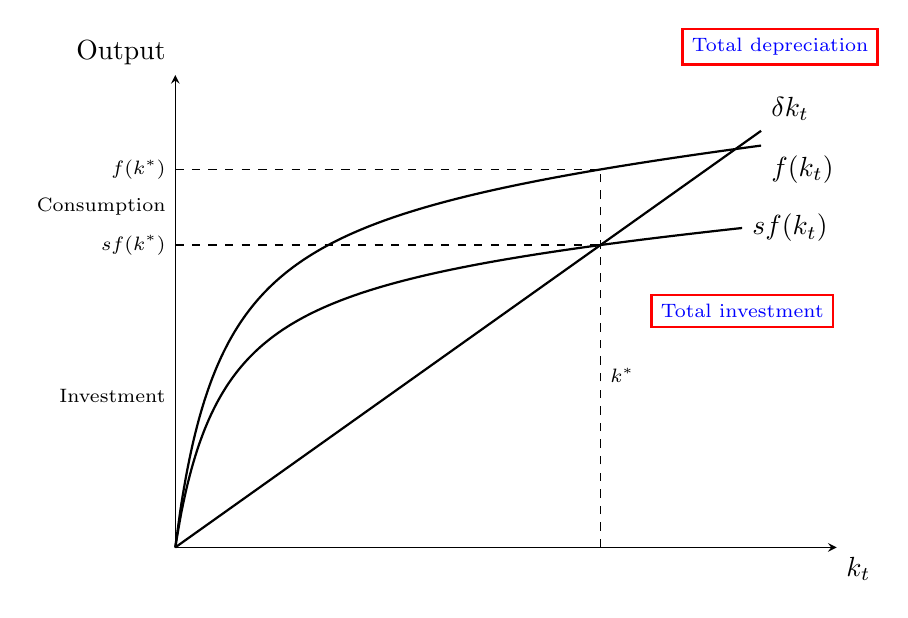
\begin{tikzpicture}[>=stealth, scale=1.2]

        % Draw axes
        \draw[->] (0,0) -- (7,0) node[below right] {$k_t$};
        \draw[->] (0,0) -- (0,5) node[above left] {Output};
        
        % Draw the curves
        \draw[thick,domain=0:6.2,samples=100,smooth,variable=\x] plot ({\x},{4*\x/(0.5+\x) + 0.4/4.5*\x}) node[below right] {$f(k_t)$};
        \draw[thick,domain=0:6,samples=100,smooth,variable=\x] plot ({\x},{3.2*\x/(0.5+\x) + 0.32/4.5*\x}) node[right] {$sf(k_t)$};
        \draw[thick,domain=0:6.2] plot ({\x},{3.2/4.5*\x}) node[above right] {$\delta k_t$};
        
        % Dashed lines for steady state
        \draw[dashed] (4.5,0) -- (4.5,4) node[pos=0.5,below right] {\scriptsize $k^*$};
        \draw[dashed] (0,4) -- (4.5,4);
        \draw[dashed] (0,3.2) -- (4.5,3.2);
        
        % Labels for key points
        \node[left] at (0,4) {\scriptsize $f(k^*)$};
        \node[left] at (0,3.2) {\scriptsize $sf(k^*)$};
        
        % Annotations with boxes
        \node[draw=red, thick, fill=white] at (6.4,5.3) {\scriptsize \textcolor{blue}{Total depreciation}};
        \node[draw=red, thick, fill=white] at (6,2.5) {\scriptsize \textcolor{blue}{Total investment}};
        
        % Investment and consumption text
        \node at (0,1.6) [left] {\scriptsize Investment};
        \node at (0,3.6) [left] {\scriptsize Consumption};
    \end{tikzpicture}
    \caption{Alternative representation of Solow Model SS}
\end{figure}

\underline{Comparative statics}

At the steady state, $k^*$ satisfies:
\[\frac{f(k^*(s, \delta, A), A)}{k^*(s, \delta, A)} = \frac{\delta}{s}\]
while the differentian yields the comparative statics:
\begin{align*}
    \frac{\partial k^*(s, \delta, A)}{\partial \delta} &<0\\
    \frac{\partial k^*(s, \delta, A)}{\partial s} &>0\\
    \frac{\partial k^*(s, \delta, A)}{\partial A} &>0
\end{align*}
The higher productivity A has the 'multiplier' effect on the output directly via $k^*$.

At the steady state, the consumption per capita is:
\[c^* = c(k^*(s, \delta, A)) = (1-s) f(k^*(s, \delta, A)).\]
$s$ has two opposing effects:
\begin{itemize}
    \item Higher $s$ leads to higher $k^*$, which leads to higher $y^*$;
    \item Higher $s$ leads to lower $1-s$, which leads to lower fraction of output consumed.
\end{itemize}

Let $\hat{s}$ be the savings rate that maximizes consumption, i.e.
\[\hat{s} = \arg \max_s (1-s)f(k^*(s, \delta, A)) = \arg \max_{s} \left\{f(k^*(s, \delta, A)) - \delta k^*(s, \delta, A)\right\}.\]
Hence $\hat{s}$ is implicitly defined by:
\[f^{\prime} (k^*(\hat{s}, \delta)) = \delta. \]

\begin{definition}[Golden Rule]\label{Golden Rule}
    \

    The Golden Rule is the savings rate that maximizes consumption in the steady state,
    which is $\hat{s}$ in our model. And, we have $k^{gold} = f'^{-1}(\delta)$ as
    the golden rule capital stock.

    \begin{note}
        \ 

        \begin{itemize}
            \item Savings are excessive if depreciation is higher than the marginal
            product of capital;
            \item By saving less, consumption go up;
            \item The economy is dynamically inefficient if $k>k^{gold}$.
        \end{itemize}
    \end{note}
\end{definition}

\subsection{Growth in the Solow Model}

Dynamics is fully determined by the evolution of capital:
\begin{align*}
    g_k(t) &= \frac{k_{t+1} - k_t}{k_t}\\
    &= \frac{(1-\delta)k_t + sf(k_t) - k_t}{k_t}\\
    &= s\frac{f(k_t)}{k_t}-\delta\\
    &= g_k(k_t)
\end{align*}
So, in the long run, the growth rate of capital is constant and equal to $\frac{sf(k^*)}{k^*} - \delta$.
As long as $k_t<k^*$, the growth rate of capital is positive, and vice versa.

\subsection{The Growing Economy}

Now we extend the model to the situation where $A_t$ and $L_t$ grow over time. 
In the previous section, the long-run outcome was the steady state where there is no growth.
This extension is necessary for addressing the facts related to the growth issues described in later chapters.

We assume that the aggregate production function takes the form of
\[
Y_t = F(K_t, A_t L_t).
\]
There are two changes from the basic model: 
first, we allow the labor input (population times hours worked per person) $L_t$ to grow over time. 
Second, and more importantly, we allow for technological progress. 
In this production function, the variable representing the technology level, $A_t$, 
is multiplied by labor input $L_t$. 
Technological progress thus takes a form of improving the labor input, 
and $A_t L_t$ is often referred to as the total number of efficiency units of labor (or effective labor). 

This form of technological progress is labor-augmenting; it was introduced in the previous chapter. 
As was also asserted there, Uzawa (1961) proved that labor-augmenting technical change is the only form of technical progress that is consistent with exact balanced growth, 
that is, the growth path where aggregate variables such as output and capital grow at a constant rate. 
% Uzawa's theorem is formally stated and proved in Appendix 3.A.

We assume that the (net) growth rate of $A_t$ is $\frac{\dot{A_t}}{A_t} = g$ and that the growth rate of $L_t$ is $\frac{\dot{L_t}}{L_t} = n$. The same manipulations of equations as in the basic model yield
\[
K_{t+1} = (1 - \delta)K_t + sF(K_t, A_t L_t).
\]
The dynamic equation for capital in continuous time is
\[
\dot{K_t} = sF(K_t, A_t L_t) - \delta K_t.
\]
Let us define the efficient unit of capital $k_t$ by
\[
k_t = \frac{K_t}{A_t L_t}.
\]
and take the log derivative w.r.t. time,
\[
\frac{\dot{k_t}}{k_t} = \frac{\dot{K_t}}{K_t} - \frac{\dot{A_t}}{A_t} - \frac{\dot{L_t}}{L_t} = \frac{\dot{k_t}}{k_t} - g - n.
\]
Output per efficiency unit of labor is:
\[
\hat{y_t} = \frac{Y_t}{A_t L_t} = F(k_t, 1) = f(k_t).
\]
Here, $f(k_t) = F(k_t, 1)$ as in the basic model. Hence, the above equation can be written as:
\begin{align*}
    \frac{\dot{k_t}}{k_t} &= \frac{sF(K_t, A_t L_t) - \delta K_t}{K_t} - g - n\\
    &= \frac{sF(K_t, A_t L_t)}{K_t} - (\delta + g + n) \\
    &= \frac{sf(k_t)}{k_t} - (\delta + g + n).
\end{align*}
Therefore, we can get the dynamic of efficient capital $k_t$ as
\[
\dot{k_t} = sf(k_t) - (\delta + g + n)k_t.
\]
After the capital stock $K_t$ is normalized by $A_t L_t$, 
we thus obtain a very similar difference equation as the fundamental equation in the basic model,
with effective depreciation rate $\delta + g + n$.

In this case, upon entering a balanced growth path, 
the rate of per capita output growth depends uniquely on the rate of technological progress $g$.

\subsection{Growth effects of changes in the savings rate}
Consider the consumption path $c^*$ per unit of effective labor, especially in the context of returning to equilibrium and whether the consumption level per unit of effective labor will be above, below, or equal to the level during the previous equilibrium.

This analysis depends on a proposition: an increase in the savings rate persistently raises the average capital stock per unit of effective labor, as well as savings and output levels. The question then arises whether it also implies an increase or decrease in the consumption level per unit of effective labor. Under what conditions does consumption per unit of effective labor reach its optimum?

\underline{Impact of Savings Rate Changes on Optimal Consumption per Unit of Effective Labor}

The formula:
\begin{align*}
    c^* &= f(k^*) - s f(k^*) = f(k^*) - (n + g + \delta) k^* \\
    \frac{\partial c^*}{\partial s} &= \left[f'(k^*(s, n, g, \delta)) - (n + g + \delta) \right] \frac{\partial k^*}{\partial s}
\end{align*}
reveals that whether an increase in the savings rate leads to a long-term rise in consumption per unit of effective labor 
depends on the comparison between the marginal product of capital at the steady-state per capita capital stock and the slope of the investment schedule. 

This formula assists in addressing the query raised in the consumption path analysis diagram.

When the long-term steady-state capital stock per unit of effective labor satisfies the condition that $f^{\prime} (k^*) = n + g + \delta$, 
\textit{the capital stock per unit of effective labor} reaches the golden-rule(\ref{Golden Rule}) level, 
and \textit{the consumption per unit of effective labor is optimal}.

\underline{Impact of Changes in the Savings Rate on the Output of Steady-State Efficient Labor, Capital Stocks}

A rise in the savings rate can lead to a change in the amount of capital in steady state efficient labor:
\begin{align*}
s f(k^*(s,n,g,\delta)) &= (n + g + \delta) k^*(s,n,g,\delta) \\
f(k^*(s,n,g,\delta)) + s f'(k^*) \frac{\partial k^*}{\partial s} &= (n + g + \delta) \frac{\partial k^*}{\partial s} \\
\frac{\partial k^*}{\partial s} = \frac{f(k^*)}{(n + g + \delta) - s f'(k^*)} &> 0
\end{align*}

The sensitivity of the steady state capital per effective labor to the savings rate is crucial. Under the condition that the derivative \(s'f(k^*)\) is smaller than \((n + g + \delta)\), implying that the change in the steady state capital stock \(dk^*/ds < 0\), an increase in the savings rate will initially reduce the consumption per effective worker until new equilibrium is achieved.

Further, the change in production per effective labor \(y^*\) with respect to the savings rate is given by:
\begin{align*}
\frac{\partial y^*}{\partial s} &= f'(k^*) \frac{\partial k^*(s, n, g, \delta)}{\partial s} = \frac{f^{\prime}(k^*) f(k^*)}{(n + g + \delta) - sf^{\prime}(k^*)} > 0
\end{align*}

Finally, the response of production per effective labor to changes in the savings rate can be expressed as:
\begin{align*}
    \frac{s}{y^*} \frac{\partial y^*}{\partial s} &= \frac{s}{f(k^*)} \frac{f^{\prime}(k^*) f(k^*)}{(n + g + \delta) - s f^{\prime}(k^*)} \\
    &= \frac{(n+g+\delta) k^* f^{\prime}(k^*)}{f(k^*) \left[(n+g+\delta) - (n+g+\delta) k^* f^{\prime}(k^*) / f(k^*)\right]} \\
    &= \frac{k^* f^{\prime}(k^*) / f(k^*)}{1 - k^* f^{\prime}(k^*) / f(k^*)} \\ 
    &= \frac{\alpha_k(k^*)}{1 - \alpha_k(k^*)}
    \end{align*}
where \( \alpha_k(k^*) \) represents the output elasticity of capital at the steady state. 
This equation helps in determining whether the increase in the savings rate will eventually 
increase the consumption level per unit of effective labor in the long run.

\begin{summary}
    \

    \begin{itemize}
        \item Baseline Model: 
            \begin{itemize}
                \item No long-run growth, i.e. capital accumulation alone does not make
                the economy grow in the long run
                \item Conditional convergence: if countries have the same parameters $s, \delta, A$
                and the same production function $F$, they will converge to the same
                steady state. Countries further from the steady state will grow faster.
                \item Crucial mechanism: decreasing marginal product to capital
            \end{itemize}
        \item Extended Model:
            \begin{itemize}
                \item Long-run growth poible if productivity grows: $g>0$;
                \item Consistant with Kaldor facts if $g>0$;
            \end{itemize}
        But $s$ and $g$ are exogenous.
    \end{itemize}
\end{summary}

\section{Development Accounting}
Development accounting asks whether the factors of production can explain income levels(See Caselli 2005\cite{caselli2005accounting}).

Assuming the production function is Cobb-Douglas in physical and human capital(more general than labor):
\begin{align*}
    Y_j &= A_j K_j^{\alpha} (L_j h_j)^{1-\alpha}\\
    y_j &= F(k_j, h_j, A_j) = A_j k_j^{\alpha} h_j^{1-\alpha} = A_j y_j^{KH} 
\end{align*}
Casselli(2005) use the following method to measure success:
\[\text{success} = \frac{\var\left[ \log(y_j^{KH} )\right] }{\var\left[\log(y_j)\right]}.\]
Then, if all countries had the same technology $A_j$, then the success would be 1.

How to measure human capital? Not directly observable. But: can
see distribution of schooling in the population, and can see
individual's wage and schooling.

From the production function
\[Y_j = K_j^{\alpha} (A_j H_j)^{1-\alpha}\]
we can calibrate the relative productivity differences relative to the US as
\[\frac{A_j}{A_{US}} = \left(\frac{Y_j}{Y_{US}}\right)^{\frac{1}{1-\alpha}} \left(\frac{K_{US}}{K_{j}}\right)^{\frac{\alpha}{1-\alpha}} \frac{H_{US}}{H_j}.\]

\nocite{*} % Add this line to include all entries in the bibliography
\chapter{Neoclassical Growth Model}
\section{Open Economy with Capital}
\chapter{Real Business Cycle Model(1)}
\section{Introduction}
Why do we have aggregate fluctuations (booms \& recessions)?

What can we do against them?

\subsection{Review of Undergrad Macro}
Economy divided into three markets: labor market, money market,
goods market.
\begin{itemize}
  \item IS: $Y = \underset{Demand for good}{\underbrace{A(Y, r, T, Y^{\prime e}, r^{\prime e}, T^{\prime e} )}} + G$
  \item LM: $M = P\cdot L(Y, i)$
  \item PC: $\pi = \pi^e + \underset{Deviation of output from MR level}{\underbrace{f(Y, z)}}$
\end{itemize}
where $Y^{\prime e}$ is the expected output of the next period, $r = i - \pi^e$ is the real expected interest rate.

\subsection{Assumptions / implications of this model}
In the short run the price level, $P$ is given, hence IS and LM determines output. Demand matters and many factors affect demand.

In the medium run, $\pi^e = \pi$, so $f(Y, z) = 0$, output at the natural level. 

money affects output in the short run, not in the medium run:
\begin{itemize}
  \item money growth affects inflation and the nominal rate
  one-for-one in the medium run
  \item a fiscal expansion increases output in the short run, may
  decrease it in the medium run
  \item expectations matter: an anticipated fiscal contraction can be
  expansionary
\end{itemize}

\subsection{Strength and weakness of these models}
\begin{itemize}
  \item Strengths:
    \begin{itemize}
      \item provides a simple way of thinking about general equilibrium
      (complicated)
      \item implicit micro-foundations: life cycle, q theory,...
      \item time-tested shortcuts (but often not based on empirical
      evidence)
    \end{itemize}
  \item Weakness:
    \begin{itemize}
      \item Static, not dynamic
      \item not really made for quantitative analysis (quantitative
      attempts very short-lived)
      \item need explicit micro-foundations: hard to do welfare analysis
      without that (Lucas critique: curves may not be invariant to
      policy)
    \end{itemize}
\end{itemize}

\subsection{Business Cycle Facts}

\textbf{Business Cycle Facts I}

We'll study the \textbf{detrended macro times series:}
\[ x_t = \log (X_t) - \log (X_t^{\ast}) \]
is the percentage deviation of variable $X$ from its trend $X^{\ast}$.

How's the trend?

\begin{enumerate}
  \item[1.] First linear,
  
  \item[2.] more sophisticated filters: Baxter-King(Bankpass) filter,
  Hodrick-Prescott(HP) filter
\end{enumerate}

Linear: just run OLS regression and use residuals.

\textbf{Business Cycle Facts II:}
Look at the highest correlation with GDP:
\[
\rho(X_t, Y_{t+k}) \quad k = -6, -5, \dots, 0, \dots, 5, 6
\]
\begin{itemize}
  \item if $\rho > 0$, then $x$ is pro-cyclical.
  \item if $\rho < 0$, then $x$ is counter-cyclical.
  \item if $k < 0$, then $x$ lags behind output.
  \item if $k > 0$, then $x$ leads output.
\end{itemize}
$\rho(X_t, X_{t+k})$ is called the autocorrelation function (as a function of $k$) of the stochastic process $X_t$.

\textbf{Business Cycle Facts III:}

Governmetn spending, not strongly correlated with level of output, main driver
of business cycles.

Real wage is mildly pro-cyclical: average wage evolves differently than the
wage of a continuously employed worker.

\textbf{\textbf{Business Cycle Facts IV:}}

Standard deviations (unit of measure is percentage deviation from
trend).

\begin{itemize}
  \item GDP is more volatile than consumption
  \item investment is much more volatile than GDP
  \item government spending is pretty volatile
  \item working hours is almost exactly as volatile as GDP
  \item vast majority of the volatility of working hours is explained by
  the employment volatility
  \item TFP is very volatile
\end{itemize}

\subsection{Towards the RBC Model}
First, it's important to state the assumptions of our economic model:
\begin{itemize}
  \item We will use a Walrasian model.
  \item The model assumes perfectly competitive markets.
  \item There are no externalities, asymmetric information, missing markets, or other imperfections.
\end{itemize}

\textcolor{blue}{\textbf{Choice of Model}}

All the neoclassical models reviewed so far share these assumptions. A familiar model that could be built upon is the Ramsey model:
\begin{itemize}
  \item The Ramsey model is known for converging to a balanced growth path in the absence of shocks, following which it exhibits smooth growth.
\end{itemize}

\textcolor{blue}{\textbf{Model Extensions}}

It appears sensible to extend the Ramsey model to incorporate:
\begin{itemize}
  \item Business cycle fluctuations.
  \item Real economic shocks.
\end{itemize}
These extensions will enhance the model's capability to reflect dynamic economic changes.

\textcolor{blue}{\textbf{Factors to Consider}}

In extending the model, the following factors should be considered:
\begin{itemize}
  \item Worker productivity.
  \item Government purchases.
\end{itemize}
Notably, since the Ramsey model does not incorporate monetary aspects, all introduced shocks will be in real terms, affecting the actual productive capacity of the economy.

\textcolor{blue}{\textbf{The Real Business Cycle (RBC) Model}}

The modified version of the Ramsey model, incorporating real shocks and business cycle fluctuations, is known as the Real Business Cycle (RBC) model.

\section{The Basic RBC Model}

\subsection{Preparation}
We take the Cobb-Douglas production function as the basis for our model:
\[ Y_t = K_t^{\alpha} (A_t L_t)^{1 - \alpha} \]
Define the technological progress as:
\[ A_t = A_t^* \tilde{A}_t \]
where $A_t^* = G^t \overline{A} $ is the long-run non-stochastic log-linear trend $G>1$.

shock process is an autoregressive process of order 1
\[\log \tilde{A}_t = \rho \log \tilde{A}_{t-1} + \varepsilon_{A, t} \]
where $\varepsilon_{A, t} \sim N(0, \sigma^2)$.

The capital accumulation equation is:
\[ K_{t+1} = (1 - \delta) K_t + I_t \]
where $I_t = Y_t - C_t$ is the investment.

Define the household's utility function as:
\[ U = \mathbb{E}_t \sum_{i=0}^{\infty} \beta^i U(C_{t+i}, 1-L_{t+i} )\]
where $\beta$ is the discount factor, $C$ is consumption, and $L$ is fraction of time spent working.

$U_C (C, 1 - L) > 0, U_{C C} (C, 1 - L) < 0$ and $U_L (C, 1 - L) > 0$, $U_{L
L} (C, 1 - L) < 0$

\subsection{The Household's Problem}

\begin{align*}
  \max_{\{C_t, L_t, K_t, S_t\}} & \quad \mathbb{E}_t \sum_{i=0}^{\infty} \beta^i U(C_{t+i}, 1 - L_{t+i}) \\
  \text{Subject to:} & \quad S_{t+i} + C_{t+i} = \tilde{R}_{t+i} K_{t+i} + W_{t+i} L_{t+i} \\
  & \quad K_{t+i+1} = (1 - \delta) K_{t+i} + S_{t+i} \\
  & \quad K_{t+i} \geq 0; \quad K_0 > 0
\end{align*}
Define the Lagrangian as:
\[
\mathcal{L} = \mathbb{E}_t \sum_{i=0}^{\infty} \beta^i U(C_{t+i}, 1 - L_{t+i}) - \mathbb{E}_t \sum_{i=0}^{\infty} \beta^i \lambda_{t+i} (K_{t+i+1} - (1 - \delta) K_{t+i} - \tilde{R}_{t+i} K_{t+i} - W_{t+i} L_{t+i} + C_{t+i})
\]
We want to take a snapshot of how the variables behave in the period in which we are optimising
in, $t$. Then, the period $t$ variables appear as:
\begin{align*}
  \mathcal{L}_t &= U(C_{t}, 1 - L_{t}) - \lambda_{t} (K_{t+1} - (1 - \delta) K_{t} - \tilde{R}_{t} K_{t} - W_{t} L_{t} + C_{t})
\end{align*}

\subsubsection{Household Behavior I}

The inter-temporal Euler equation is:
\[U_1(X_t, 1-L_t) = \beta \mathbb{E}_t \left(R_{t+1} U_1(C_{t+1}, 1-L_{t+1} ) \right)\]
where $R_{t+1} = 1 + \tilde{R}_{t+1} - \delta $.

\subsection{Effect of RBC}

What are the effects of a positive technological shock?

It increases current and future $R$ and $W$.
\subsubsection{Consumption}
\begin{itemize}
  \item \textbf{Income effect:} People feel richer which leads to an increase in consumption.
  \item \textbf{Substitution effect:} Saving is worth more, thus consumption might decrease.
  \item \textbf{Net effect:} Consumption is probably increased.
\end{itemize}

\subsubsection{Leisure}
\begin{itemize}
  \item \textbf{Income effect:} People feel richer, thus they want to enjoy more leisure, leading to an increase in leisure.
  \item \textbf{Substitution effect:} Higher wage leads to a decrease in leisure.
  \item \textbf{Net effect:} The overall impact on leisure depends on the relative strength of the two effects.
\end{itemize}

\subsubsection{Type of Shock}
\begin{itemize}
  \item \textbf{Transitory shock:} Leads to a smaller wealth effect and a stronger substitution effect.
  \item \textbf{Permanent shock:} It is possible that consumption goes up and employment goes down.
\end{itemize}

\subsection{Brief Summary}
\begin{itemize}
  \item Consumption is too pro-cyclical;
  \item investment $I_t = s_t Y_t = \alpha \beta Y_t$ also pro-cyclical;
  \item effects of R on saving?
  $r$ increase, then inter-temporal substitution effect led $C_t$ decreases, 
  then the income effect increases $C_t$(in this model they cancel out)
  \item $W_t$ is too pro-cyclical
\end{itemize}
\chapter{Review Session 2024.10.17}
\section{A simplified real-business cycle model with additive technology shocks}

\begin{problem}[1]
    Find the first-order condition (Euler equation) relating $C_t$ and $C_{t+1}$ in the following model:
\end{problem}

\begin{solution}
    The household's problem is to maximize
    \begin{equation*}
        \max_{\{C_t\}} E_{t} \sum_{t=0}^{\infty} u(C_t)/{(1+\rho)^t}
    \end{equation*}
    subject to the budget constraint
    \begin{equation*}
        K_{t+1} = K_t + Y_t - C_t
    \end{equation*}
    where $Y_t = A K_t + e_t$ and $e_t$ is a random technology shock satisfying $e_t = \phi e_{t-1} + \epsilon_t $, $-1 < \phi < 1$ and that $\epsilon_t$ is \textbf{i.i.d}.

    Define the Lagrange function:
    \begin{equation}
        \mathcal{L} = E_t  \sum_{t=0}^{\infty} \left[ u(C_t)/{(1+\rho)^t} - \lambda_t (K_{t+1} - K_t - Y_t + C_t) \right]
    \end{equation}
    The first-order condition with respect to $C_t$ is:
    \begin{equation}
        \frac{\partial \mathcal{L}}{\partial C_t} = 0 \Rightarrow \frac{u'(C_t)}{(1+\rho)^{t} } - \lambda_t = 0
    \end{equation}

    The first-order condition with respect to $K_{t+1}$ is:
    \begin{equation}
        \frac{\partial \mathcal{L}}{\partial K_{t+1}} = 0 \Rightarrow -\lambda_{t} + E_t\left[\lambda_{t+1}\right](1+\rho) = 0
    \end{equation}
    Combining (2) and (3) we get:
    \begin{equation}
        \frac{u'(C_t)}{(1+\rho)^{t} } = E_t\left[\lambda_{t+1}\right](1+\rho)
    \end{equation}
    We have the relationsjip between $C_t$ and $C_{t+1}$:
    \begin{equation}
        u'(C_t) = E_t\left[u'(C_{t+1})\right]
    \end{equation}
    Since $u(C_t) = C_t - \theta C_t^2$, we have $u'(C_t) = 1 - 2\theta C_t$. Thus, the Euler equation is:
    \begin{equation}
        1 - 2\theta C_t = E_t\left[1 - 2\theta C_{t+1}\right] \Rightarrow C_t = E_t\left[C_{t+1}\right]
    \end{equation}
\end{solution}

\begin{problem}[2]
    Guess that consumption takes the form$ C_t = \alpha  + \beta K_t + \gamma e_t$. What's $K_t$ in this case?
\end{problem}

\begin{solution}
    \begin{align*}
        K_{t+1} &= K_t + Y_t - C_t \\
        &= K_t + (A K_t + e_t) - \alpha - \beta K_t - \gamma e_t \\
        &= (1+A-\beta) K_t - \alpha + (1-\gamma) e_t
    \end{align*}
\end{solution}

\begin{problem}[3]
    What values must the parameters $\alpha $, $\beta$ , and $\gamma$ have for the first-order condition in part 1 to be
satisfied for all values of $K_t$ and $e_t$?
\end{problem}

\begin{solution}
    From the Euler equation, we have:
    \begin{equation}
        C_t = E_t\left[C_{t+1}\right]
    \end{equation}
    Substituting $C_t = \alpha  + \beta K_t + \gamma e_t$ and $C_{t+1} = \alpha  + \beta K_{t+1} + \gamma e_{t+1}$ into (7), we get:
    \begin{equation}
        \alpha  + \beta K_t + \gamma e_t = E_t\left[\alpha  + \beta K_{t+1} + \gamma e_{t+1}\right]
    \end{equation}
    Rearranging using $$E_t\left[e_{t+1}\right] = E_t \left[\phi e_t + \epsilon \right] = \phi e_t.$$
    Substituting $K_{t+1} = (1+A-\beta) K_t - \alpha - (1-\gamma) e_t$ into (8), we get:
    \begin{equation}
        \alpha  + \beta K_t + \gamma e_t = E_t\left[\alpha  + \beta ((1+A-\beta) K_t - \alpha + (1-\gamma) e_t) + \phi\gamma e_{t} + \gamma \epsilon_t \right]
    \end{equation}
    Simplifying (9) we get:
    \begin{align*}
        \alpha  + \beta K_t + \gamma e_t &= \alpha  + \beta (1+A-\beta) K_t - \alpha \beta  + \beta (1-\gamma) e_t + \phi\gamma e_{t} + \gamma E_t\left[\epsilon_t\right] \\
        \Rightarrow \beta K_t + \gamma e_t &= \beta (1+A-\beta) K_t - \alpha \beta  + \beta (1-\gamma) e_t + \phi\gamma e_{t} \\
    \end{align*}
    Hence, we have:
    \begin{align*}
        \alpha \beta  &= 0 \\
        \beta &= \beta (1+A-\beta) \\
        \gamma &= \beta (1-\gamma) + \phi\gamma
    \end{align*}
    SOlving the above equations, we get:
    \begin{align*}
        \alpha &= 0 \\
        \beta &= A = \rho \\
        \gamma &= \frac{\beta}{1+\beta -\phi} = \frac{A}{1+A -\phi}
    \end{align*}
\end{solution}

\begin{problem}[4]
    What are the effects of a one-time shock to $\epsilon $ on the paths of $Y$, $K$, and $C$?
\end{problem}

\begin{solution}
    \begin{equation}
        K_{t+1} = (1+A-\beta) K_t - \alpha + (1-\gamma) e_t = K_t + \frac{1-\phi}{1+A-\phi}e_t
    \end{equation}
    Thus, we can have:
    \begin{align*}
        K_{t+T} &= K_t + \sum_{j=0}^{T-1} \frac{1-\phi}{1+A-\phi}e_{t+j} \\
        &= K_t + \frac{1-\phi}{1+A-\phi} \sum_{j=0}^{T-1} \phi^j e_{t} \\
        \Rightarrow \lim_{T \to \infty} K_{t+T} &= K_t + \frac{1}{1+A-\phi} e_t
    \end{align*}

    For $C_t$:
    \begin{align*}
        C_t &= \alpha  + \beta K_t + \gamma e_t \\
        &= A K_t + \frac{A}{1+A-\phi} e_t
    \end{align*}
    \begin{align*}
        C_{t+1} &= A K_{t+1} + \frac{A}{1+A-\phi} e_{t+1} \\
        &= A \left[K_t + \frac{1-\phi}{1+A-\phi}e_t\right] + \frac{A}{1+A-\phi} e_{t+1}  \\
        &= A K_t + \frac{A(1-\phi )}{1+A-\phi} e_t + \frac{A}{1+A-\phi} e_{t+1} 
    \end{align*}
    Similarly,
    \begin{align*}
        C_{t+T} &= A K_{t+T} + \frac{A}{1+A-\phi} e_{t+T} \\
        &= A K_t + \frac{A}{1+A-\phi} \sum_{t=0}^{T-1} \phi^j e_t \\
        \Rightarrow \lim_{T \to \infty} C_{t+T} &= A K_t + \frac{A}{1+A-\phi} \phi^T e_t + \frac{A}{1+A-\phi} e_t
    \end{align*}
\end{solution}



\section{Solving the RBC model by finding the social optimum}

\begin{problem}[1]
    Explain the Bellman equation:
    \begin{equation}
        V(K_t, A_t) = \max_{C_t, L_t} \left\{\log{C_t} + b\log{(1-L_t)} + \beta E_t \left[V(K_{t+1}, A_{t+1})\right] \right\}
    \end{equation}
\end{problem}

\begin{solution}
    
\end{solution}

\begin{problem}[2]
    Given the log-linear structure of the model, let us guess that $V$ takes the form:
    $$V\left(K_t,A_t\right)=\gamma_0+\gamma_K\log K_t+\gamma_A\log A_t$$

    where the values of the $\beta$'s are to be determined. Substituting this conjectured form and the facts
    that $K_{t+1}=Y_t-C_t$ and $E_t\left[\log A_{t+1}\right]=\rho\log A_t$ into the Bellman equation yields
    $$V\left(K_t,A_t\right)=\max_{C_t,L_t}\left\{\log C_t+b\log\left(1-L_t\right)+\beta\left[\gamma_0+\gamma_K\log\left(Y_t-C_t\right)+\gamma_A\log A_t\right]\right\}.$$
    Find the frst-order condition for $C_t.$ Show that it implies that $C_t/Y_t$ does not depend on $K_t$ or $A_t.$
\end{problem}

\begin{solution}
    Based on our value function, the first-order condition for $C_t$ is:
    \begin{equation}
        \frac{\partial V}{\partial C_t} = 0 \Rightarrow \frac{1}{C_t} = \beta \gamma_K \frac{1}{Y_t - C_t} \Rightarrow \frac{C_t}{Y_t} = \frac{1}{1 + \beta \gamma_K}        
    \end{equation}
    Hence, $C_t/Y_t$ does not depend on $K_t$ or $A_t$.
\end{solution}

\begin{problem}[3]
    Find the first-order condition for $L_t.$ Use this condition and the result in part 2 to show that Lt
    does not depend on $K_t$ or $A_t$.
\end{problem}

\begin{solution}
    \begin{equation}
        \frac{\partial V}{\partial L_t} = 0 \Rightarrow -\frac{b}{1-L_t} + \beta \gamma_K \frac{1}{Y_t - C_t}(1-\alpha ) K_t^{\alpha }A_t^{1-\alpha }L_t^{-\alpha }   = 0
    \end{equation}
    Simplifying (12) we get:
    \begin{equation}
        -\frac{b}{1-L_t} + \frac{\beta \gamma_K}{Y_t - C_t}(1-\alpha ) \frac{Y_t}{L_t}= 0
    \end{equation}
    Replace $Y_t - C_t$ with $\beta \gamma_K C_t$:
    \begin{align*}
        &-\frac{b}{1-L_t} + \frac{\beta \gamma_K}{\beta \gamma_K C_t}(1-\alpha ) \frac{Y_t}{L_t}= 0 \\
        \Rightarrow & \frac{1-\alpha}{L_t} (1 + \beta \gamma_K) = \frac{b}{1-L_t} \\
        \Rightarrow & L_t = \frac{(1-\alpha)(1 + \beta \gamma_K)}{(1-\alpha)(1 + \beta \gamma_K) + b}
    \end{align*}
    So, $L_t$ does not depend on $K_t$ or $A_t$.
\end{solution}

\begin{problem}[4]
    Substitute the production function and the results in questions 2 and 3 for the optimal $C_t$ and $L_t$ into the equation above for $V$, and show that the resulting expression has the form $V(K_t,A_t)=$ $\gamma_0^{\prime}+\gamma_K^{\prime}\log K_t+\gamma_A^{\prime}\log A_t.$
\end{problem}

\begin{solution}
    As we know that
    \begin{align*}
        E_t\left[\log A_{t+1}\right] &= \rho\log A_t \\
        E_t\left[K_{t+1} \right] &= \log{(Y_t - C_t)}
    \end{align*}
    So, by substituting the optimal $C_t$ and $L_t$ into the equation for $V$, we get:
    \begin{align*}
        V(K_t, A_t) &= \log{\frac{Y_t}{1+\beta \gamma_K}} + b\log{\frac{b}{(1-\alpha)(1 + \beta \gamma_K) + b}} + \beta \left\{ \gamma_0 + \gamma_K \log{\frac{\beta \gamma_K Y_t}{1 + \beta \gamma_K}} + \gamma_A \rho \log{A_t} \right\} \\
    \end{align*}
    Substitute $Y_t = K_t^{\alpha }(A_t L_t)^{1-\alpha }$, we have:
    \begin{align*}
        V(K_t, A_t) &= \alpha \log{K_t} + (1-\alpha )\log{A_t} + (1-\alpha )\log{L_t} - \log{(1+\beta \gamma_K)} \\
        &+ b\log{\frac{b}{(1-\alpha)(1 + \beta \gamma_K) + b}} + \beta \gamma_0  \\
        &+ \beta \gamma_K\left\{\log{(\beta \gamma_K)} -\log{(1+\beta  \gamma_K)} + \alpha \log{K_t} + (1-\alpha )\log{A_t} + (1-\alpha )\log{L_t} \right\} \\
        &+ \beta \gamma_A \rho \log{A_t}
    \end{align*}
    Rearranging the terms, we get:
    \begin{align*}
        V(K_t, A_t) &= (\alpha +\alpha \beta \gamma_K)\log{K_t} + (1-\alpha + (1-\alpha )\beta \gamma_K + \beta \gamma_A \rho)\log{A_t} \\
        &+ (1-\alpha + (1-\alpha )\beta \gamma_K)\log{L_t} \\
        &- \log{(1+\beta \gamma_K)} + b\log{\frac{b}{(1-\alpha)(1 + \beta \gamma_K) + b}} + \beta \gamma_0  \\
        &+ \beta \gamma_K\log{(\beta \gamma_K)} - \beta \gamma_K\log{(1+\beta  \gamma_K)}
    \end{align*}
    We define: 
    \begin{align*}
        \gamma_K^{\prime} &= \alpha (1+ \beta \gamma_K) \\
        \gamma_A^{\prime} &= (1-\alpha )(\beta \gamma_K + 1) + \beta \gamma_A \rho \\
        \gamma_0^{\prime} &= \beta \gamma_0 + b\log{\frac{b}{(1-\alpha)(1 + \beta \gamma_K) + b}} - \log{(1+\beta \gamma_K)}(1+ \beta \gamma_K) \\
        &+ \beta \gamma_K\log{(\beta \gamma_K)} + (1-\alpha + (1-\alpha )\beta \gamma_K)\log{L_t}
    \end{align*}
    According to problem 3, we know that $L_t$ does not depend on $K_t$ or $A_t$, so, we could treat it as a constant in this expression about $K_t$ and $A_t$. Thus, we have:
    \begin{align*}
        V(K_t, A_t) &= \gamma_0^{\prime} + \gamma_K^{\prime}\log{K_t} + \gamma_A^{\prime}\log{A_t}.
    \end{align*}
\end{solution}

\begin{problem}[5]
    What must $\gamma_K$ and $\gamma_A$ be so that $\gamma_K^\prime=\gamma_K$ and $\gamma_A^{\prime}=\gamma_A?$
\end{problem}

\begin{solution}
    Let $\gamma_K^{\prime} = \gamma_K$ and $\gamma_A^{\prime} = \gamma_A$, we have:
    \begin{align*}
        \gamma_K &= \alpha (1+ \beta \gamma_K) \\
        \gamma_A &= (1-\alpha )(\beta \gamma_K + 1) + \beta \gamma_A \rho \\
        \Rightarrow \gamma_K &= \frac{\alpha}{1-\alpha \beta} \\
        \Rightarrow \gamma_A &= \frac{1-\alpha}{(1-\alpha \beta)(1 -\beta \rho )}
    \end{align*}
\end{solution}

\begin{problem}[6]
    What are the implied values of $C_t/Y_t$ and $L_t$? Are they the same as those found in the lecture?
\end{problem}

\begin{solution}
    Substitute $\gamma_K$ into the expression for $C_t/Y_t$ and $L_t$, we have:
    \begin{align*}
        \frac{C_t}{Y_t} &= \frac{1}{1 + \beta \gamma_K} = \frac{1}{1 + \beta \frac{\alpha}{1-\alpha \beta}} = 1-\alpha \beta \\
        L_t &= \frac{(1-\alpha)(1 + \beta \gamma_K)}{(1-\alpha)(1 + \beta \gamma_K) + b} = \frac{(1-\alpha)}{(1-\alpha) + b(1-\alpha \beta )}
    \end{align*}

\end{solution}
\chapter{Problem Set 4}
\section*{Question 1}

Consider an RBC model with a representative household that maximizes utility
$$U_t=E_t\sum_{t=0}^\infty\beta^t\left(\log\left(C_t\right)+\nu\left(1-L_t\right)\right)$$


where $\nu$ is an increasing and concave function. The production function is
$$Y_t=A_tL_t^{1-\alpha}\left(z_tK_t\right)^\alpha $$

with $0<\alpha<1$ and $z_t$ denotes a capital utilization choice. For example, low capital utilization may mean
running the machines only at half speed or half of the time.
Capital accumulation is described by

$$K_{t+1}=\left(1-\bar{\delta}z_t^\phi\right)K_t+Y_t-C_t.$$

\begin{problem*}[1]
    Explain how variable utilitzation of capital is modeled here. Should we assume that $\phi<1$ or $\phi>1?$
\end{problem*}

\begin{solution}
    \textcolor{blue}{
        In the given model, capital utilization $z_t$ directly affects both production and capital depreciation: in the production function, $z_t K_t$ is the effective capital input at time period $t$, higher $z_t$ increases the effective capital services, thus boosting output. The depreciation rate is $\delta_t = \bar{\delta}z_t^{\phi}$, and higher $z_t$ leads to a higher depreciation rate. \\
        Depreciation Function $\delta_t = \bar{\delta}z_t^{\phi}$ determines how sensitively depreciation responds to changes in utilization $z_t$.The marginal increase in depreciation due to higher $z_t$ is given by: 
        \[
        \frac{\partial \delta_t}{\partial z_t} = \bar{\delta}\phi z_t^{\phi-1}.
        \]
        Intuitively, if utilization increases, the marginal cost of utilizing capital rises, reflecting higher incremental damage, meaning that teh capital depreciates faster, which implies:
        \[
        \frac{\partial^2 \delta_t}{\partial z_t^2} = \bar{\delta}\phi(\phi-1) z_t^{\phi-2} > 0.
        \]
        Hence, we should assume that $\phi > 1.$
    }
\end{solution}

\begin{problem*}[2]
    Derive and explain the optimality conditions of the social planner's problem. 
    The social planner's problem is to maximize total utility subject to the economy's physical resource constraints 
    (i.e. production, and the law of motion for capital). 
    The social planner can set the levels of consumption, investment, capacity utilization, and labor supply, 
    without having to worry about prices or market clearing. 
\end{problem*}

\begin{solution}
    \textcolor{blue}{
        The social planner maximizes the expected discounted utility:
        \begin{align*}
            \max_{\{C_t, I_t, L_t, z_t\}} & E_t \sum_{t=0}^\infty \beta^t \left(\log(C_t) + \nu(1-L_t)\right) \\
            \text{s.t.} \quad & Y_t = A_t L_t^{1-\alpha} (z_t K_t)^\alpha \\
            \quad \quad & K_{t+1} = (1-\bar{\delta} z_t^\phi) K_t + Y_t - C_t
        \end{align*}
        Define the Lagrangian:
        \[ 
        \mathcal{L} = E_t \sum_{t=0}^\infty \beta^t \left\{\log(C_t) + \nu(1-L_t) - \lambda_t \left[C_t + K_{t+1} - (1-\bar{\delta} z_t^\phi) K_t - Y_t\right]\right\}
        \]
        The first-order conditions are:
        \begin{align}  
            & \frac{\partial \mathcal{L}}{\partial C_t} = \beta^t (\frac{1}{C_t}-\lambda_t) = 0 \Rightarrow \frac{1}{C_t} = \lambda_t \\
            & \frac{\partial \mathcal{L}}{\partial L_t} = \beta^t\left[-\nu'(1-L_t) + \lambda_t A_t (1-\alpha) L_t^{-\alpha} (z_t K_t)^\alpha \right] = 0 \Rightarrow \nu'(1-L_t) = \lambda_t A_t (1-\alpha) L_t^{-\alpha} (z_t K_t)^\alpha \\
            & \frac{\partial \mathcal{L}}{\partial z_t} = \beta^t \lambda_t \left[ A_t \alpha L_t^{1-\alpha} z_t^{\alpha-1} K_t^\alpha - \bar{\delta} \phi z_t^{\phi-1} K_t\right] = 0 \Rightarrow \bar{\delta} \phi z_t^{\phi-1} = A_t \alpha L_t^{1-\alpha} z_t^{\alpha-1} K_t^{\alpha-1}\label{(*)} \\
            & \frac{\partial \mathcal{L}}{\partial K_{t+1}} = -\beta^t \lambda_t + \beta^{t+1}\lambda_{t+1}\left[(1-\bar{\delta}z_{t+1}^{\phi}) + \alpha \frac{Y_{t+1}}{K_{t+1}}\right] = 0 \Rightarrow \lambda_t = \beta \lambda_{t+1} (1-\bar{\delta} z_{t+1}^\phi + \alpha \frac{Y_{t+1}}{K_{t+1}})\label{(**)}
        \end{align}
        From the FOCs, we could tell that:
        \begin{enumerate}
            \item The shadow price of consumption equals to the marginal utility of consumption.
            \item For the derivative with respect to $L_t$, we can transform it into the following format: \[
            \nu'(1-L_t) = \frac{\partial Y_t}{C_t \partial L_t}
            \]
            The marginal utility of leisure equals the marginal utility gain from increased consumption made possible by supplying an extra unit of labor.
            \item For the derivative with respect to $z_t$, we can transform it into the following format:
            \[
            \frac{\partial \delta_t K_t}{\partial z_t} = \frac{\partial Y_t}{\partial z_t}
            \]
            The marginal cost(depreciation) of capital equals to the marginal gain of production of increasing capital utilization.
            \item The standard inter-temporal condition balancing current and future utility.
        \end{enumerate}
    }
\end{solution}

\begin{problem*}[3]
    Derive an expression for the steady-state capital utilization $z^*$ in terms of the steady-state capital-output ratio. If we want to normalize $z^*=1$, how should we calibrate $\phi$?
\end{problem*}

\begin{solution}
    \textcolor{blue}{
        At the steady state: $Y_t = Y$, $C_t = C$, $K_t = K$, $A_t = A$ and $L_t = L$.
        Since $C_t = C_{t+1}$, we know that $\lambda_t = \lambda_{t+1}.$
        From \ref{(*)}, we know that:
        \begin{align*}
            \alpha A L^{1-\alpha} (z^* K)^{\alpha-1} & = \phi \bar{\delta }z^{*^{\phi -1}} = \frac{\alpha Y}{z^* K} \\
            \Rightarrow \frac{Y}{K} & = \frac{\phi \bar{\delta} z^{*^{\phi }}}{\alpha}
        \end{align*}
        Denote $\kappa = \frac{K}{Y}$, which is the output ratio, we would have:
        \[
        z^* = \left( \frac{\alpha}{\kappa \phi \bar{\delta} }\right)^{\frac{1}{\phi}}.  
        \]
        Then, we use \ref{(**)} and $\lambda_t = \lambda_{t+1}$, we'll have:
        \begin{align*}
            & 1 = \beta(1 - \bar{\delta}z^{*^{\phi}} + \alpha \frac{Y}{K}) = \beta(1- \bar{\delta}z^{*^{\phi}} +\alpha \frac{\phi \bar{\delta} z^{*^{\phi }}}{\alpha} ) = \beta(1- \bar{\delta}z^{*^{\phi}} + \phi \bar{\delta} z^{*^{\phi }}) \\
            \Rightarrow & (\phi-1)\bar{\delta} z^{*^{\phi}} = \frac{1-\beta}{\beta} \\
            \Rightarrow & z^* = \left(\frac{1-\beta}{\beta (\phi-1) \bar{\delta}}\right)^{\frac{1}{\phi}}
        \end{align*}   
        Normalize $z^* = 1$, we simplify the equation into:
        \[
        1 - \beta = \beta (\phi-1) \bar{\delta},
        \]
        which gives that
        \[
        \phi = \frac{1-\beta}{\beta \bar{\delta}} + 1 = \frac{1 - \beta + \beta \bar{\delta}}{\beta \bar{\delta}}
        \]
        Or, we would simplify the expression of $z^*$ with capital-output ratio $\kappa$:
        \[
        \alpha = \kappa \phi \bar{\delta} \Rightarrow \phi = \frac{\alpha}{\kappa \bar{\delta}}
        \]
    }
\end{solution}

\begin{problem*}[4]
    Compared to a standard RBC model (as in the lecture), do you expect this model to generate a
stronger or weaker response of output to a TFP shock?
\end{problem*}

\begin{solution}
    \textcolor{blue}{
        Compared to a standard RBC model, this model generates stronger response of output to a TFP shock.\\
        \textbf{In the Standard RBC Model:}\\
        Capital utilization is fixed ($z_t=1$). Output response to TFP shocks relies solely on adjustments in labor and capital.\\
        \textbf{In This Model with Variable Utilization:}\\
        Firms can adjust $z_t$ in response to TFP shocks.
        A positive TFP shock allows firms to temporarily increase $z_t$ , boosting output beyond what is possible in the standard model, which gives higher fluctuations.
    }
\end{solution}

\begin{problem*}[5]
    Assuming the model is correct, how is the standard empirical Solow residual $\log Y_t-(1-\alpha)\log L_t-\alpha\log K_{t}$ 
    related to total factor productivity $\log A_{t}$? 
\end{problem*}

\begin{solution}
    \textcolor{blue}{
        If our model is correct, then we log-linearize the production function:
    \begin{align*}
        & \log Y_t = \log A_t + (1-\alpha)\log L_t + \alpha \log K_t + \alpha \log z_t \\
        \Rightarrow & \text{Solow Residual} = \log Y_t - (1-\alpha)\log L_t - \alpha \log K_t = \log A_t + \alpha \log z_t
    \end{align*}
    }
\end{solution}

\section*{Question 2}

We study a variation of the simplified RBC model from the lecture. Consider an economy populated by a mass of representative households and a mass of representative firms which take output and factor prices as given. The production function is Cobb-Douglas:

$$Y_t=e^{z_t}K_t^\alpha L_t^{1-\alpha}$$

where $e^z_t$ is total factor productivity, $K$ is capital, and $L$ is labor. Capital fully depreciates in every
periods so that
$$K_{t+1}=I_t$$

where $I_{t}$ is investment.

The representative household supplies labor $L_t$ and consumes $C_t.$ It maximizes

$$U=E_0\left[\sum_{t=0}^\infty\beta^t\left[\log C_t-e^{\chi_t}L_t\right]\right]$$

where $\chi_t$ is a preference shock. Capital is accumulated by the household and rented to the firm, as usual.
Any profits of the firms are rebated to the households. As usual, we have $0<\alpha<1,0<\beta<1.$

\begin{problem*}[1]
    Write down the budget constraint of the household and the profit function of firms.
\end{problem*}

\begin{solution}
    \textcolor{blue}{
        Assume the rental rate of capital is $r_t$ and the wage rate is $w_t$.
        The budget constraint of the household is:
        \[
        C_t + K_{t+1} = r_t K_t + w_t L_t + \Pi_t
        \]
        The profit function of firms is:
        \[
        \Pi_t = Y_t - r_t K_t - w_t L_t = e^{z_t} K_t^\alpha L_t^{1-\alpha} - r_t K_t - w_t L_t
        \]
    }
\end{solution}

\begin{problem*}[2]
    Derive first-order conditions of firms and households.
\end{problem*}

\begin{solution}
    \textcolor{blue}{
        From problem (1), we established:
        \[ 
        \Pi_t = Y_t - r_t K_t - w_t L_t \Rightarrow r_t K_t + w_t L_t + \Pi_t = Y_t.
        \]
        Thus, our households budget constraint is:
        \[
        C_t + K_{t+1} = Y_t.
        \]
        We define the Lagrangian of the household problem as:
        \[
        \mathcal{L} = E_0 \sum_{t=0}^\infty \beta^t \left[\log C_t - e^{\chi_t} L_t - \lambda_t (C_t + K_{t+1} - Y_t)\right].
        \]
        The first-order conditions of households are:
        \begin{align*}
            & \frac{\partial \mathcal{L}}{\partial C_t} = \beta^t (\frac{1}{C_t} - \lambda_t) = 0 \Rightarrow \frac{1}{C_t} = \lambda_t \\
            & \frac{\partial \mathcal{L}}{\partial L_t} = \beta^t (-e^{\chi_t} + \lambda_t \frac{\partial Y_t}{\partial L_t}) = 0 \Rightarrow e^{\chi_t} = \lambda_t \frac{\partial Y_t}{\partial L_t}\\
            & \frac{\partial \mathcal{L}}{\partial K_{t+1}} = -\beta^t \lambda 
            _t + \beta^{t+1}E_t \lambda_{t+1} \frac{\partial Y_{t+1}}{\partial K_{t+1} } = 0 \Rightarrow \lambda_t = \beta \lambda_{t+1} E_t \frac{\partial Y_{t+1} }{\partial K_{t+1} }
        \end{align*}
        Let's compute $\frac{\partial Y_t}{\partial L_t}$ and $\frac{\partial Y_t}{\partial K_{t+1} }$:
        \begin{align*}
            & \frac{\partial Y_t}{\partial L_t} = e^{z_t} K_t^\alpha (1-\alpha) L_t^{-\alpha} = (1-\alpha) \frac{Y_t}{L_t} \\
            & \frac{\partial Y_{t+1} }{\partial K_{t+1} } = \alpha e^{z_{t+1} } K_{t+1}^{\alpha-1} L_{t+1}^{1-\alpha} = \alpha \frac{Y_{t+1} }{K_{t+1} }
        \end{align*}
        So, our households FOCs are:
        \begin{align}
            & \lambda_t = \frac{1}{C_t}\label{1.1} \\
            & e^{\chi_t} = \lambda_t (1-\alpha ) \frac{Y_t}{L_t} = \frac{(1-\alpha )Y_t}{C_t L_t}\label{1.2} \\
            & \lambda_t = \alpha \beta \lambda_{t+1} E_t \frac{Y_{t+1} }{K_{t+1} } \Rightarrow \frac{1}{C_t} = \alpha \beta E_t \frac{Y_{t+1} }{C_{t+1} K_{t+1} }\label{1.3}
        \end{align}
        The Lagrangian of the firm problem is:
        \[
        \max_{K_t, L_t} \Pi_t = e^{z_t} K_t^\alpha L_t^{1-\alpha} - r_t K_t - w_t L_t
        \]
        The first-order conditions of firms are:
        \begin{align}
            & \frac{\partial \Pi_t}{\partial K_t} = \alpha e^{z_t} K_t^{\alpha-1} L_t^{1-\alpha} - r_t = 0 \Rightarrow r_t = \alpha e^{z_t} K_t^{\alpha-1} L_t^{1-\alpha} = \alpha \frac{Y_t}{K_t}\label{1.4} \\
            & \frac{\partial \Pi_t}{\partial L_t} = (1-\alpha) e^{z_t} K_t^\alpha L_t^{-\alpha} - w_t = 0 \Rightarrow w_t = (1-\alpha) e^{z_t} K_t^\alpha L_t^{-\alpha} = (1-\alpha )\frac{Y_t}{L_t}\label{1.5}
        \end{align}
    }
\end{solution}

\begin{problem*}[3]
    Show that when factor markets and final good markets are competitive, firm profits are zero.
\end{problem*}

\begin{solution}
    \textcolor{blue}{
        The competitive equilibrium requires that the rental rate of capital equals the marginal product of capital and the wage rate equals the marginal product of labor:
    \begin{align*}
        & r_t = \alpha \frac{Y_t}{K_t}  \\
        & w_t = (1-\alpha) \frac{Y_t}{L_t}
    \end{align*}
    In this case, the profit function of firms becomes:
    \[
    \Pi_t = Y_t - \alpha \frac{Y_t}{K_t} K_t - (1-\alpha) \frac{Y_t}{L_t} L_t = 0.
    \]
    }
\end{solution}

\begin{problem*}[4]
    Solve the model and show that the process for output in a competitive equilibrium is
    $$y_t=z_t+\alpha y_{t-1}-(1-\alpha)\chi_t$$ 
    (where lowercase letters denote the log of the uppercase letter).
\end{problem*}

\begin{solution}
    \textcolor{blue}{
        From the production function FOC \ref{1.3}, we have:
        $\frac{1}{C_t} = \alpha \beta E_t \frac{Y_{t+1} }{K_{t+1}C_{t+1}}.$
        Since $Y_{t+1} = C_{t+1} + I_{t+1} = C_{t+1} + K_{t+2}$, We have: 
        \begin{align*}
            \frac{1}{C_t} &= \alpha \beta E_t \frac{C_{t+1} + K_{t+2}}{K_{t+1}C_{t+1}} \\
            \Rightarrow \frac{K_{t+1} }{C_t} &= \alpha \beta E_t \left(1 + \frac{K_{t+2} }{C_{t+1} }\right)
        \end{align*} 
        \textcolor{red}{According to the Banach's Fixed-point Theorem}, $x = \alpha \beta (1+x)$, and we can solve \[\frac{K_{t+1}}{C_t} = \frac{\alpha \beta }{1-\alpha \beta}.\]\\
        As $K_{t+1} = Y_t - C_t$, we have $K_{t+1} = \alpha \beta Y_t $ and $C_t = (1-\alpha \beta )Y_t$.
        Then, by \ref{1.2} and \ref{1.5}, we know that:
        \begin{align*}
            e^{\chi _t} &= \frac{(1-\alpha )Y_t}{C_t L_t} \\
            \Rightarrow e^{\chi _t} &= \frac{(1-\alpha )Y_t}{(1-\alpha \beta )Y_t L_t} = \frac{1-\alpha }{1-\alpha \beta } \frac{1}{L_t} \\
            \Rightarrow L_t &= \frac{1-\alpha }{1-\alpha \beta }e^{-\chi _t}
        \end{align*} 
        \[Y_t = e^{z_t}K_t^\alpha L_t^{1-\alpha} = e^{z_t}(\alpha \beta Y_{t-1} )^\alpha \left(\frac{1-\alpha }{1-\alpha \beta }e^{-\chi _t}\right)^{1-\alpha}\]
        The the log of both sides, we have:
        \begin{align*}
            \log Y_t &= z_t + \alpha \log (\alpha \beta ) + \alpha \log Y_{t-1} + (1-\alpha )\log \left(\frac{1-\alpha }{1-\alpha \beta }\right) - (1-\alpha )\chi _t \\
            &= z_t + \alpha \log Y_{t-1} - (1-\alpha )\chi _t + \alpha \log (\alpha \beta ) + (1-\alpha )\log \left(\frac{1-\alpha }{1-\alpha \beta }\right)\\
            \Rightarrow y_t &= z_t + \alpha y_{t-1} - (1-\alpha )\chi _t + \alpha \log (\alpha \beta ) + (1-\alpha )\log \left(\frac{1-\alpha }{1-\alpha \beta }\right)
        \end{align*}
        We drop the constant and gives: $y_t = z_t + \alpha y_{t-1} - (1-\alpha )\chi _t.$
    }
\end{solution}

\begin{problem*}[5]
    Assume $y_{-1}=0$ and $z_t=0$ for all $t$, and $\chi_t=0$ for all $t$ except that $\chi_0=1\%.$ Draw the time path
for $\chi_{t},z_{t}$,and $y_{t}.$ Explain why $y_{t}$ is persistent.
\end{problem*}

\begin{solution}
    \ 

    \textcolor{blue}{
        At time period 0, $y_0 = z_0 + \alpha y_{-1} - (1-\alpha )\chi _0 = 1\%(\alpha-1)$, and after time period 0, we have $z_t = 0$ and $\chi_t = 0$, thus $y_t = \alpha y_{t-1} = 1\% \alpha^t(\alpha -1).$ Then, we can draw the three graphs as below:
    }
    
    % Graph 1
    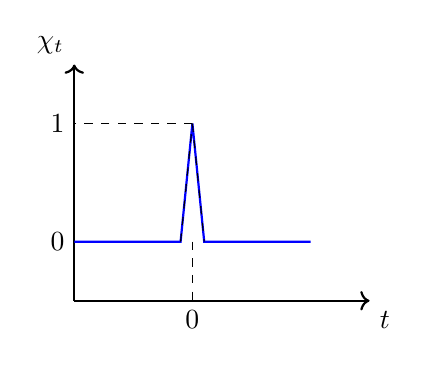
\begin{tikzpicture}[scale=1.5]
        % Axes
        \draw[thick,->] (0,0) -- (2.5,0) node[anchor=north west] {$t$};
        \draw[thick,->] (0,0) -- (0,2) node[anchor=south east] {$\chi _t$};
    
        % Plot
        \draw[thick, blue] (0,0.5) -- (0.9,0.5) -- (1,1.5) -- (1.1,0.5) -- (2,0.5);
    
        % Dashed lines
        \draw[dashed] (1,1.5) -- (0,1.5) node[anchor=east] {1};
        \draw[dashed] (1,0.5) -- (1,0) node[anchor=north] {0};
        \draw[dashed] (0.9,0.5) -- (1,1.5);
        \draw[dashed] (1,1.5) -- (1.1,0.5);
    
        % Labels
        % \node[below] at (1,0) {$0$};
        \node[left] at (0,0.5) {$0$};
    \end{tikzpicture}
        % Graph 2
    \begin{tikzpicture}[scale=1.5]
        \draw[thick,->] (0,0) -- (2.5,0) node[anchor=north west] {$t$};
        \draw[thick,->] (0,0) -- (0,2) node[anchor=south east] {$z_t$};
        \draw[thick, blue] (0,1) -- (2.2,1);
        \draw[dashed] (0,0.3) -- (0,0.3) node[anchor=east] {};
        \node[left] at (0,1) {0};
    \end{tikzpicture}
    % Graph 3
    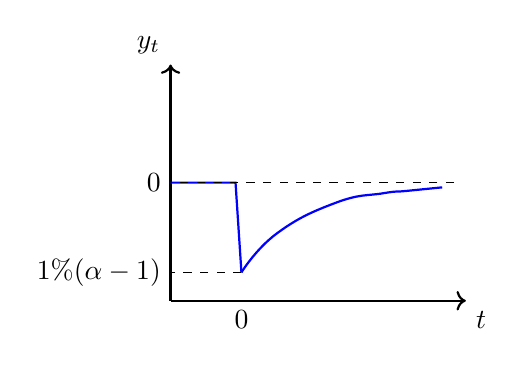
\begin{tikzpicture}[scale=1.5]
        \draw[thick,->] (0,0) -- (2.5,0) node[anchor=north west] {$t$};
        \draw[thick,->] (0,0) -- (0,2) node[anchor=south east] {$y_t$};
        \draw[thick, blue] (0,1) -- (0.55,1) -- (0.6,0.24);
        \draw[thick, blue] plot[smooth, tension=0.8] coordinates {(0.6,0.24) (0.9,0.57) (1.4,0.83) (1.8,0.91) (2.0, 0.93) (2.3,0.96)};
        \draw[dashed] (2.4,1) -- (0,1) node[anchor=east] {0};
        \draw[dashed] (0.6,0.24) -- (0,0.24) node[anchor=east] {$1\%(\alpha -1)$};
        \node[below] at (0.6,0) {0};
    \end{tikzpicture}
    
    \textcolor{blue}{
        The initial preference shock $\chi _0$ increases the disutility of labor, leading households to supply less labor at $t=0$. \\
        This reduces output at $t=0$.\\
        Since capital at $t+1$ depends on savings from $Y_t$ , the reduced output leads to lower capital $K_{t+1}$. \\
        The lower capital stock in subsequent periods reduces output further, even though the preference shock is gone.\\
        The capital accumulation process transmits the shock over time, causing persistence in output deviations from steady state.\\
        But as the shock has ended, the output will finally return back to the steady state.
    }
\end{solution}
\chapter{Real Business Cycle Model(2)}
\section{From Advanced Economies (AE) to EMDEs}

We saw that a calibrated version of the SOE-RBC model captures well
key empirical regularities of a developed SOE like Canada (chapter 4).
\begin{question}
    Can the OE-RBC model also explain business cycles in EMDEs?
\end{question}

\begin{note}
    A quick reminder of the SOE-RBC Model:
    \begin{align*}
        \max \quad & E_0 \sum_{t=0}^{\infty}\beta ^t U(c_t, h_t) \\
        s.t. \quad & d_t + A_t F(k_t, h_t) = (1+r_{t-1} )d_{t-1} +c_t + k_{t+1} - (1-\delta)k_t + \Phi(k_{t+1} - k_t) \\
    \end{align*}
    and a non-Ponzi game constraint.
\end{note}

In theory, we can get higher volatility of every component by increasing $\epsilon$, or we can make consumption more volatile than output if we increasr
$\rho $.

The more persistent the shock is, the longer income stays above the steady state.
If the permanent income increase greatly, the consumption will respondingly increase.

\begin{intuition}
    \ 

    \begin{itemize}
        \item In principle, the SOE-RBC model can easily handle this difference.
        \item Simply jack up (by a factor of around 2) the standard deviation of the productivity shock. After all, in the SOE-RBC model, $\sigma _a$ was calibrated to match the standard deviation of Canadian GDP.
        \item Since not only output but also all of the components of aggregate demand (consumption, investment, net exports) are more volatile in
        EMDEs than in AEs, increasing $\sigma _a$ would help along more than one dimension.
        \item But in models with just one exogenous shocks, up to first order, the
        ratio of two standard deviations is independent of the standard
        deviation of the exogenous shocks
    \end{itemize}
\end{intuition}

\subsection{The SOE-RBC Model With Nonstationary Technology Shocks: Consumption}

The HH problem:
\[
\max \quad E_0\sum_{t=0}^\infty\beta^t\frac{[C_t^\gamma(1-h_t)^{1-\gamma}]^{1-\sigma}-1}{1-\sigma}
\]
subject to the standard NPG $$\lim_{j\to\infty}E_t\frac{D_{t+j+1}}{\Pi_{s=0}^j(1+r_{t+s})}\leq0$$ and

$$\frac{D_{t+1}}{1+r_t}+Y_t=D_t+C_t+K_{t+1}-(1-\delta)K_t+\frac\phi2\left(\frac{K_{t+1}}{K_t}-g\right)^2K_t,$$

\begin{itemize}
    \item Most variables and parameters as before.
    \item We now have a Cobb-Douglas period utility index instead of GHH. 
    \item Debt takes the form of one-period discount bonds. The HH receives $\frac{D_{t+1}}{(1+r_t)}$ units ot
    good in period $t$ and needs to repay $D_t+1$ in period $t+1.$ (for the HH, there is no difference between this formulation and the one introduced before, to see this set $D_t^{\prime}=D_t/(1+r_{t-1}).$
    \item Also: $\beta$, and $\delta$ are between 0 and 1 and $\gamma,\sigma,\phi$,and $g(g$ is the gross growth rate
    of $X$ in a non-stochastic equilibrium path; $X$ will be defined next page) are
positive
\end{itemize}

Set up the Lagrangean and get:

\begin{align*}
    & \frac{1-\gamma}\gamma\frac{C_t}{1-h_t}=(1-\alpha)a_tX_t\left(\frac{K_t}{X_th_t}\right)^\alpha \\
    & \gamma C_t^{\gamma(1-\sigma)-1}(1-h_t)^{(1-\gamma)(1-\sigma)}=\Lambda_t\\
    & \Lambda_t=\beta(1+r_t)E_t\Lambda_{t+1}
\end{align*}
\[
\Lambda_{t}\left(1+\phi\left(\frac{K_{t+1}}{K_{t}}-g\right)\right)=\beta E_{t}\Lambda_{t+1}\left[1-\delta+\alpha a_{t+1}\left(\frac{K_{t+1}}{X_{t+1}h_{t+1}}\right)^{\alpha-1}+\phi\frac{K_{t+2}}{K_{t+1}}\left(\frac{K_{t+2}}{K_{t+1}-g}\right)-\frac{\phi}{2}\left(\frac{K_{t+2}}{K_{t+1}-g}\right)^{2}\right]
\]

$\Lambda_t$ is the Lagrange multiplier associated with the sequential budget
constraint of the household.


\chapter{Money and the New Keynesian Model}
\section{About Monetary Economics}

Does an unanticipated shock to money affect real side of the
economy (quantities)?

\begin{itemize}
    \item CLassical view: If prices are flexible, the shock
    will change wages and prices proportionally, but not change the quantities.

    If the gov prints money and spend it, the prices increase and nominal assets lose in value, 
    which is negative wealth effect.

    Money supply increase acts like a tax on nominal asset 
    holdings, some call it 'inflation tax'.

    \item Keynesian view: Prices are rigid, so the shock will
    give a positive wealth effect, this assumes that new money is distributed proportionally to existing money holdings.
\end{itemize}

How should we conduct monetary policy?

\begin{itemize}
    \item Monetatists: steady money supply growth, in line with money
    demand growth.
    \item Keynesians: use expansionary MP to stimulate the economy
    in a recession.
    \item Inflation of 70's and subsequent successful tight MP(Volcker)
    led to Monetarists becoming very influential.
\end{itemize}

\textcolor{blue}{Problems of previous models}

\begin{itemize}
    \item Old models are subject to the Lucas critique(policy changes
    may affect people's response to the policies)
    \item Hard to take seriously from a quantitative perspective
\end{itemize}

Since RBC model has try to use dynamic method to explain the economy, 
people start putting money into the model.

\begin{itemize}
    \item Outcome from this program is the “New Keynesian
    Synthesis”: combine RBC models with price rigidities.
    \item Money is non-neutral in the short run (Keynesian
    element), and neutral in the long run (classical element).
\end{itemize}

\section{The Monetary Transmission Mechanism}

\subsection{Households and nominal assets}

Nominal assets are bonds $B_t$ which pay interest at nominal rate $i_t$.
Ignore the labor-leisure choice, the households maximize:
\begin{align*}
    \max & \quad \mathbb{E}_t \sum_{i=0}^{\infty}U(C_{t+i} )\\
    \text{s.t.} & \quad P_{t+i}C_{t+i} + P_{t+i}K_{t+i+1} + B_{t+i+1} = W_{t+i}L + P_{t+i}(1+r_{t+i})K_{t+i} + (1+i_{t+i})B_{t+i} 
\end{align*}
where $W$ is the nominal wage, $P$ is the price of cunsumption goods,
$r_{t+i}$ is the rental rate of capital net of depreciation.

Define the Lagrangian:
\begin{align*}
    \mathcal{L} = \mathbb{E}_t\sum_{i=0}^{\infty} \left[ U(C_{t+i} ) + \lambda_{t+i} \left( W_{t+i}L + P_{t+i}(1+r_{t+i})K_{t+i} + (1+i_{t+i})B_{t+i} - P_{t+i}C_{t+i} - P_{t+i}K_{t+i+1} - B_{t+i+1} \right) \right]
\end{align*}

The FOCs are:
\begin{align*}
    U^{\prime} (C_{t+i} ) &= \mathbb{E}_t P_{t+i}\lambda_{t+i}  \\
    P_{t+i}\lambda_{t+i} &= \mathbb{E}_t \lambda_{t+i+1} P_{t+i+1} (1+r_{t+i+1}) \\
    \lambda_{t+i} &= \mathbb{E}_t \lambda_{t+i+1} (1+r_{t+i+1}) \\
\end{align*}
Combining the first two, we get the standard Euler equation:
\[
    U^{\prime} (C_{t} ) = \mathbb{E}_t \left(U^{\prime} (C_{t+1} ) (1+r_{t+1})\right)
\]
Conbine the first and the third:
\[
    U^{\prime} (C_{t} ) = \mathbb{E}_t \left(\frac{1+i_{t+1}}{1+\pi_{t+1}} U^{\prime} (C_{t+1} )\right)
\]
where inflation $\pi = \frac{P_{t+1} - P_t}{P_t}$.

\begin{align*}
    U^{\prime} (C_{t} ) &= \mathbb{E}_t \left(\frac{1+i_{t+1}}{1+\pi_{t+1}} U^{\prime} (C_{t+1} )\right) \\\\
    U^{\prime} (C_{t} ) &= \mathbb{E}_t \left((1+r_{t+1}) U^{\prime} (C_{t+1} )\right) \\\\
\end{align*}

\begin{itemize}
    \item What matters for the intertemporal consumption decision is
    the real interest rate, not the nominal interest rate.
    \item The FOC are necessary conditions for having both positive $B$
    and positive $K$. By the two equations above, we get:
    \[1+r_{t+1} = \frac{1+i_{t+1}}{1+\pi_{t+1}}. \]
    So, the \textcolor{red}{real return(interest rate)} of a nominal asset
    with \textcolor{red}{nominal interest rate} $1+i_{t+1} $ is: $\frac{1+i_{t+1} }{1+\pi_{t+1}}$.
    % \item This is the Fisher equation.
\end{itemize}

\begin{corollary}[Fisher equation]
    \ 

    It's the relationship between asset returns that has to hold 
    so that the household is willing to hold positive amounts 
    of these assets in their portfolio (or: if you allow negative 
    holdings, to clear asset markets). \\
    When households are risk-neutral, the FOCs become:
    \[\mathbb{E}_t (1+r_{t+1}) = \mathbb{E}_t \left(\frac{1+i_{t+1}}{1+\pi_{t+1}}\right) \]
    In a deterministic world, there's no $E$, which is often approxima
\end{corollary}

\subsection{Firms}
The firms would like to maximize profits, with perfect competition adn frictionless factor markets:
\[MPK = r\]
Again, real interest rate matters. 

\textbf{Conclusion:} if monetary policy should affect demand, the real interest rate is the key price in the economy.

\section{The tools of monetary policy}
So, in order to stimulate demand, the central bank needs to change the real interest rate.

\subsection*{How?}

\begin{itemize}
    \item Change the money supply, with demand curve, this would implement a particular nominal interest rate.
    \item Change the nominal interest rate directly.
\end{itemize}

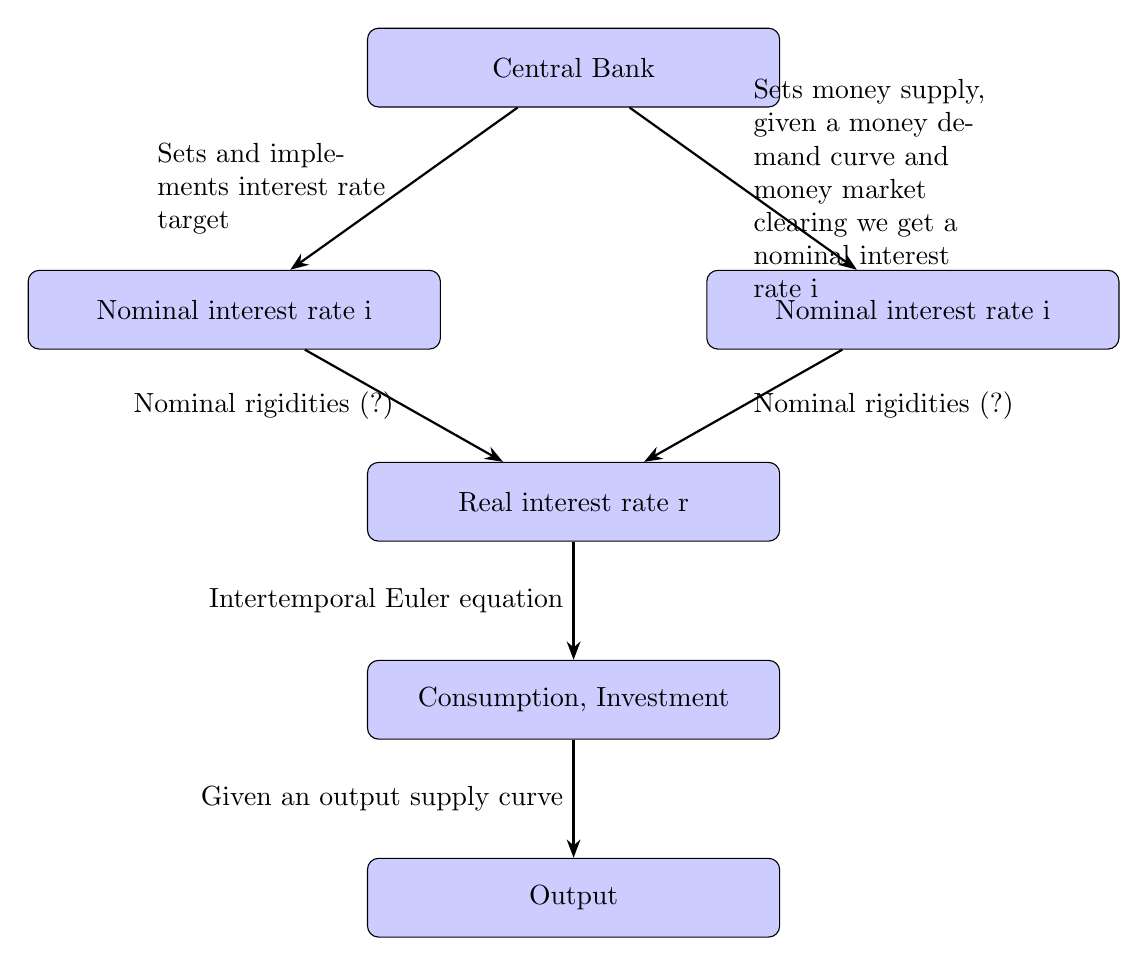
\begin{tikzpicture}[
    node distance=1.5cm,
    block/.style={
        rectangle,
        draw,
        fill=blue!20,
        text width=5cm,
        text centered,
        rounded corners,
        minimum height=1cm
    },
    arrow/.style={
        thick,
        ->,
        >=Stealth
    }
]

% Nodes
\node (centralbank) [block] {Central Bank};

% First branch
\node (nominalrate1) [block, below left=of centralbank, xshift=2cm, yshift=-1cm] {Nominal interest rate i};

% Second branch
\node (nominalrate2) [block, below right=of centralbank, xshift=-2cm, yshift=-1cm] {Nominal interest rate i};

% Combined branch
\node (realrate) [block, below=of centralbank, yshift=-3cm] {Real interest rate r};
\node (consumption) [block, below=of realrate] {Consumption, Investment};
\node (output) [block, below=of consumption] {Output};

% Arrows for the first branch
\draw [arrow] (centralbank) -- (nominalrate1) node[midway, left, text width=3cm, align=left] {Sets and implements interest rate target};
\draw [arrow] (nominalrate1) -- (realrate) node[midway, left] {Nominal rigidities (?)};

% Arrows for the second branch
\draw [arrow] (centralbank) -- (nominalrate2) node[midway, right, text width=3cm, align=left] {Sets money supply, given a money demand curve and money market clearing we get a nominal interest rate i};
\draw [arrow] (nominalrate2) -- (realrate) node[midway, right] {Nominal rigidities (?)};

% Arrows for the combined branch
\draw [arrow] (realrate) -- (consumption) node[midway, left] {Intertemporal Euler equation};
\draw [arrow] (consumption) -- (output) node[midway, left] {Given an output supply curve};

\end{tikzpicture}

\subsection*{Money supply-demand equilibrium}

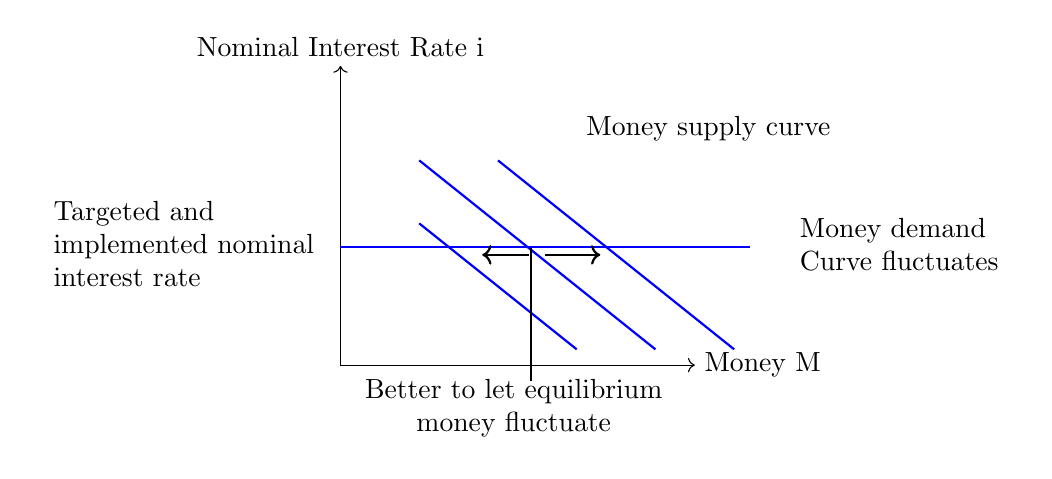
\begin{tikzpicture}[scale=1]
    \draw[->] (0,0) -- (4.5,0) node[right] {Money M};
    \draw[->] (0,0) -- (0,3.8) node[above] {Nominal Interest Rate i};
    
    % Money demand curves
    \draw[blue, thick] (1,2.6) -- (4,0.2);
    \draw[blue, thick] (2,2.6) -- (5,0.2);
    \draw[blue, thick] (1,1.8) -- (3,0.2);
    
    % % Money supply curve (vertical line)
    \draw[black, thick] (2.42,1.5) -- (2.42,-0.2);
    
    % Horizontal line for targeted interest rate
    \draw[blue, thick] (0,1.5) -- (5.2,1.5);
    
    % Arrows showing fluctuation
    \draw[->, thick] (2.4,1.4) -- (1.8,1.4);
    \draw[->, thick] (2.6,1.4) -- (3.3,1.4);
    
    % Labels
    \node[left] at (0,1.5) {\begin{tabular}{l}Targeted and\\implemented nominal\\interest rate\end{tabular}};
    \node[below] at (2.2,0) {\begin{tabular}{c}Better to let equilibrium\\money fluctuate\end{tabular}};
    \node[right] at (3,3) {Money supply curve};
    \node[right] at (5.5,1.5) {\begin{tabular}{l}Money demand\\Curve fluctuates\end{tabular}};
\end{tikzpicture}

\section{A model of the interbank market}
\begin{itemize}
    \item Market participants: $n$ banks.
    \item Banks hold reserves at the central bank.
    \item REserves are used for settling transfers between banks arising from the payment system.
    \item Banks are unsure of the transfers htey will need to make.
    \item Banks can borrow reserves from one another in the interbank market,
    but do not know how much reserve they'll require at the point they participate in the interbank market.
    \item Banks can also acquire reserves through the repo (repurchase
    agreement) market. The central bank can be a participant in
    this market.
\end{itemize}

\begin{note}
    \ 

    $B_j$ = reserves of bank $j$ at beginning-of-period.(after previous debts settles) \\
    $I_j$ = net borrowing in the interbank market (negative for
    lending) by bank $j$. \\
    $P_j$ = net bond repos(sales and repurchases) by bank $j$. \\
    $T_j$ = net payment bank $j$ make to other banks. \\
    $R_j$ = balance of bank $j$ at end-of-period. \\
    Accounting: $R_j = B_j + I_j + P_j - T_j$.
\end{note}

\subsection{Interbank market and repo market}
\textbf{Interbank market:}
\begin{itemize}
    \item Uncollateralized loans between banks.(银行间无抵押贷款, potentially risky)
    \item Interest rate $i$.
\end{itemize}

\textbf{Repo market:}
\begin{itemize}
    \item Sell bond now and agree to repurchase later.
    \item Effectively a collaboratized loan, so risk-free if collateral is good.
\end{itemize}

\begin{note}[Central bank facilities]
    \ 

    \textbf{Deposit Facility:} Centrla bank offers an interest rate of $i_d$ on deposit balances in banks' account at the end of time period.

    \textbf{Borrowing facility:} Central bank charges an interest rate $i_b$ on negative balances in banks' accounts.
    \begin{itemize}
        \item Positive spread over deposit rate: $i_b > i_d$.
        \item Equivalent to an offer to make loans at the end of perios, with the oad credited to the bank's account.
        \item Collateral required -- we should assune banks have enough collateral to use it.
    \end{itemize}
\end{note}

\subsection{Balance on account next period}

Reserve balance of bank $j$ at the end of period is:
\[
B^{\prime} _j = R_j - (1+i)(I_j + P_j) + \left\{\begin{matrix}
   i_d R_j & \text{if } R_j \geq 0\\
   i_b R_j & \text{if } R_j < 0
  \end{matrix}\right.
\]
Since $R_j = B_j + I_j + P_j - T_j$, we have:
\[
B^{\prime} _j = B_j - T_j - i(I_j + P_j) + \left\{\begin{matrix}
   i_d (B_j + I_j + P_j - T_j) & \text{if } B_j + I_j + P_j - T_j \geq 0\\
   i_b (B_j + I_j + P_j - T_j) & \text{if } B_j + I_j + P_j - T_j < 0
  \end{matrix}\right.
\]

Assume banks are risk-neutrala, and they aim to maximize their next period expected balance $\mathbb{E}(B^{\prime}_j)$.
Choice variabls are: interbank transaction $I_j$, repo market transaction $P_j$.
\begin{align*}
    \mathbb{E}(B^{\prime}_j) = B_j - i(I_j + P_j) &+ i_d \int_{-\infty}^{B_j + I_j + P_j} (B_j + I_j + P_j - T_j) dF(T_j) \\
    &+ i_b \int_{B_j + I_j + P_j}^{\infty} (B_j + I_j + P_j - T_j) dF(T_j)
\end{align*}
The FOCs are:
\begin{align*}
    \frac{\partial \mathbb{E}(B^{\prime}_j)}{\partial I_j} &= 0 \\
    \frac{\partial \mathbb{E}(B^{\prime}_j)}{\partial P_j} &= 0
\end{align*}

Two equations lead to the same equation, so we only consider one of them.
\begin{theorem}[Leibniz Rule]
    \ 
    
    Let $f(x, t)$ be a function such that both $f(x, t)$ and 
    its partial derivative $f_x(x, t)$ are continuous in $t$ and 
    $x$ in some region of the $xt$-plane, 
    including $a(x) \leq t \leq b(x)$, $x_0 \leq x \leq x_1$. 
    Also suppose that the functions $a(x)$ and $b(x)$ are both continuous 
    and both have continuous derivatives for $x_0 \leq x \leq x_1$. 
    Then, for $x_0 \leq x \leq x_1$,
    \[
    \frac{d}{dx} \left( \int_{a(x)}^{b(x)} f(x, t) \, dt \right) = f(x, b(x)) \cdot \frac{d}{dx} b(x) - f(x, a(x)) \cdot \frac{d}{dx} a(x) + \int_{a(x)}^{b(x)} \frac{\partial}{\partial x} f(x, t) \, dt.
    \]
\end{theorem}

Use the Leibniz rule:
\begin{align*}
    & \frac{\partial}{\partial I_j} \int_{-\infty}^{B_j + I_j + P_j} (B_j + I_j + P_j - T_j) dF(T_j) \\
    &= \int_{-\infty}^{B_j + I_j + P_j} f(T_j)d T_j + \left((B_j + I_j + P_j) - (B_j + I_j + P_j)\right)f(B_j + I_j + P_j) \\
    &= F(B_j + I_j + P_j) 
\end{align*}
Similarly,
\begin{align*}
    & \frac{\partial}{\partial I_j} \int_{B_j + I_j + P_j}^{\infty} (B_j + I_j + P_j - T_j) dF(T_j) \\
    &= 1 - F(B_j + I_j + P_j)
\end{align*}
Hence, the FOC reduces to:
\[
-i + i_d F(B_j + I_j + P_j) + i_b (1 - F(B_j + I_j + P_j)) = 0
\]
Equivalently,
\[
(i - i_d)F(B_j + I_j + P_j) = (i_b - i)(1 - F(B_j + I_j + P_j))
\]
The optimal demand for interbank and repo lending is characterized by the equation: 
\[
F(B_j + I_j + P_j) = \frac{i_b - i}{i_b - i_d}
\]

\subsection{Aggregation and market clearing}
\begin{align*}
    B &= \sum_{j=1}^{n}B_j (\text{Aggregate beginning-of-period balances})\\
    P &= \sum_{j=1}^{n}P_j (\text{Aggregate end-of-period balances})\\
    T &= \sum_{j=1}^{n}T_j = 0 (\text{payments between banks cancel out})  \\
    R &= \sum_{j=1}^{n}R_j
\end{align*}

Since $R_j = B_j + I_j + P_j - T_j$, we have $R = B+P$ in the aggregate.

Since $B_j + I_j + P_j$ is the same for all banks: $B_j + I_j + P_j = \frac{R}{n}$.

\subsection{Equilibrium interbank interest rate}
\begin{align*}
    F\left(\frac{R}{n}\right) &= \frac{i_b - i}{i_b - i_d} \\
    \frac{R}{n} &= F^{-1}\left(\frac{i_b - i}{i_b - i_d}\right) \\
    i &= i_d + \frac{i_b - i_d}{n} \int_{-\infty}^{F^{-1}\left(\frac{i_b - i}{i_b - i_d}\right)} x dF(x)
\end{align*}

THe central bank directly controls:
\begin{itemize}
    \item $i_d$ and $i_b$.
    \item Open market operations $P$.
\end{itemize}
Indirectly determinems
\begin{itemize}
    \item Interbank and repo rate $i$.
    \item Total end-of-period reserves $R = B+P$.
\end{itemize}

\subsection{Interbank market with channel system}
\begin{itemize}
    \item \textbf{Demand:} Equation $F\left(\frac{R}{n}\right) = \frac{i_b - i}{i_{b-i_d}}$, giving a negative relationship between $i$ and $R$.
    \item \textbf{Supply:} Central bank sets $R = B+P$ by open market operations.
\end{itemize}

If we hold all other policy instruments constant,
\begin{itemize}
    \item An increase in total reserves $R$ will shift supply curve to the right, decreasing $i$.
    \item An increase in $i_d$ will shift demand curve upward, increasing $i$.
    \item An increase in $i_b$ will shift demand curve upward, increasing $i$.
\end{itemize}

\begin{note}
    \ 

    A narrow channel has advantages:
    \begin{itemize}
        \item More precise control of $i$, less fluctuations.
        \item Less need for open market operations.
    \end{itemize}

    There'are also disadvantages, e.g. $i_b = i_b$:
    \begin{itemize}
        \item Trading in interbank market dries up.
        \item CB becomes the intermediary of all borrowing and lending between banks, hence it incurs the cost of monitoring credit-worthiness of banks. \textcolor{red}{It's not the central bank's job.}
    \end{itemize}
\end{note}

\subsection{Interest rate maturity}

\begin{question}
    How does this affect medium- and long-term interest rates? How are interest rates of different maturities related?
\end{question}

\begin{eg}
    \ 

    Imagine an investor invest for 2 years:
    \begin{itemize}
        \item Buy a 2-year bond, keep until it matures: \[\text{return} = 1 + i_t^{(2y)}\]
        \item Buy a 1-year bond, then buy another 1-year bond: \[\text{return} = (1+i_t^{(1y)})(1+i_{t+1}^{1y})\]    
    \end{itemize}

    \textbf{Expectations Hypothesis:} Expectations of these two returns should be the same:
    \[i_t^{(2y)} = \mathbb{E}_t (1 + i_t^{(1y)})(1 + i_{t+1}^{(1y)}).\]

    This should hold exactly if agents are risk-neutral. WIth risk aversion, one would adjust the expected retuen for riskiness.
\end{eg}

\chapter{Problem Set 5}
\section*{Question 1}

Consider the model of the interbank market presented in the lectures. i is the interbank interest rate, id
is the interest rate offered by the central bank on positive balances on banks' reserve accounts (deposit
rate), ib is the interest rate charged by the central bank on negative reserve balances (borrowing rate).
Banks face uncertainty about the payments they must make after the interbank market has closed. The
probability that a bank's required payment is less than $T$ is denoted by $F(T)$. Optimization by banks
implies the following condition:
\[(i_b - i)\left(1 - F(R/n)\right)= (i -i_d)F(R/n)\] 
or equivalently:
\[F(R/n) = \frac{i_b - i}{i_{b} - i_d}\]
where $R$ is the total quantity of reserves and $n$ is the number of banks.

\begin{problem*}[1]
    Provide an intuitive explanation of the optimality condition for banks.
\end{problem*}

\begin{solution}
    
\end{solution}

\begin{problem*}[2]
    Show how the equilibrium interbank interest rate is determined using a diagram.
\end{problem*}

\begin{solution}
    The conditions gives that:
    \[
    F(R/n) = \frac{i_{b} -i}{i_{b} -i_d} \in [0, 1] \Rightarrow i_d \leq i \leq i_{b} .
    \]
    If the inter-bank rate 
    \begin{figure*}[h!]
        \centering
        \includegraphics*{figures/PS5(2).png}
    \end{figure*}
\end{solution}

\begin{problem*}[3]
    Suppose the central bank would like to raise the market interest rate.
    Explain how this can be done through:

        (a) Open market operations (only R is adjusted);

        (b) Adjusting standing facility terms (only ib and id are adjusted)
\end{problem*}

\begin{solution}
    Originally, the graph changes as the following graph:
    
    \begin{figure*}[h!]
        \centering
        \includegraphics*{PS(3).png}
    \end{figure*}

    Let's suppose the bank increase rate by $x$, say $i^{\prime} =i+ x$.
    \[ 
    F(R/n) = \frac{(i_{b} +x) - (i+x)}{(i_{b} +x) - (i_d +x)} = \frac{i_{b} ^{\prime} -i^{\prime} }{i_{b} ^{\prime} -i_d^{\prime}}
    \]
    \begin{figure*}[h!]
        \centering
        \includegraphics*{figures/PS(3)-2.png}
    \end{figure*}
\end{solution}


\section*{Question 2}
You are hired by the International Monetary Fund, and you're being assigned on a mission to provide
technical assistance to Bank al-Maghrib, the central bank of Morocco. You're being asked to estimate
the impact of monetary policy on unemployment. Knowing that your boss is not fond of DSGE models,
but also distrusts the results from Christiano-Eichenbaum-Evans (because they were obtained with data
from high-income countries), you decide to estimate a Vector Autoregression model (with interest rates
and unemployment as the endogenous variables) yourself.

\begin{problem*}[1]
    Write down the system of equations for a first-order Vector Autoregression 
    where the nominal interest rate and unemployment depend on each other 
    and a lagged variable for each. Both variables are also determined by a shock, 
    $\eta_t^i$ and $\eta_t^u$ , which are orthogonal to past values of $i$ and $u$.
\end{problem*}

\begin{solution}
    \begin{align*}
        i_t &= \phi_1 i_{t-1} + \phi_2 u_t + \phi_3 u_{t-1} + \eta_t^i \\
        u_t &=\phi_4 i_t + \phi_5 u_{t-1} + \phi_6 i_{t-1} + \eta_t^u \\
        & cov(x_{i_t}, \epsilon_{i_t}) = 0
    \end{align*}
    \[
    \Rightarrow i_t = \phi_1 i_t + \phi_2(\phi_4 i_{t-1} + \phi_5 u_{t-1} + \phi_6 i_{t-1} + \eta_t^u) + \phi_3 u_{t-1} + \eta_t^i
    \]
    Solve the equation, we have:
    \begin{align*}
        i_t &= \frac{1}{1-\phi_2 \phi_4} \left[(\phi_{1}+\phi_2 \phi_6)i_{t-1} + (\phi_{3}+\phi_2 \phi_5)u_{t-1} + \phi_2 \eta_t^u + \eta_t^i\right] \\
        u_t &= \frac{1}{1-\phi_2 \phi_4} \left[(\phi_{1} \phi_4 +\phi_6)i_{t-1} + (\phi_{3}\phi_4 +\phi_5)u_{t-1} + \phi_4 \eta_t^i + \eta_t^u\right] \\
        \epsilon_{i_t} &= \frac{1}{1-\phi_2 \phi_4}\left[\phi_2 \eta_t^u + \eta_t^i\right] \\
        \epsilon_{u_t} &= \frac{1}{1-\phi_2 \phi_4}\left[\phi_4 \eta_t^i + \eta_t^u\right]
    \end{align*}
    If we guess $\phi_4 = 0$, we have:
    \begin{align*}
        \epsilon_t^i &= \eta_t^i + \phi_2 \eta_t^u\\
        \epsilon_t^u &= \eta_t^u \\
        \Rightarrow \epsilon_t^i &= \phi_2 \epsilon_t^u + \eta_t^i 
    \end{align*}

\end{solution}
\chapter{New Keynesian Model}
Start off with baseline RBC model, add a nominal asset(one-period bond)

Price stickiness only makes sense when firms can set prices;
hence, need some degree of market power. Special case of
Rotemberg \& Woodford.

Nominal rigidities: Calvo pricing: firm-specific shock that tells
you whether you're allowed to reset your price.

\section{Households}
\begin{align*}
    \max &\quad \mathbb{E}_0 \sum_{i=0}^\infty \beta^i \left[ u(c_{t+1}) - \nu(l_{t+i} ) \right] \\
    \text{s.t.} &\quad p_tc_t + b_t = (1+i_{t-1})b_{t-1} + p_t w_t l_t + p_t d_t
\end{align*}
where $c_t$ is quantity of baskets of goods consumed, $p_t$ is the prive of each basket in terms of money,
$d_t$ is the real wage, $d_t$ are dividends(firms' profits) received from owning firms,
$i_t$ is the nominal interest rate, $b_t$ is the quantity of nominal bonds held by the household.

The intertemporal optimality condition is as follows:
\begin{align*}
    u'(c_t) = \beta \mathbb{E}_t(1+r_t)u'(c_{t+1})
\end{align*}
where $r_t$ is the real interest rate given by: $1 + r_t = \frac{1+i_t}{1+\pi_{t+1} }$
and $\pi_{t+1} = \frac{p_{t+1}-p_t}{p_t}$ is the inflation rate between $t$ and $t+1$.

Labor supply is given by:
\begin{align*}
    MRS_{l,c} = \frac{\nu'(l_t)}{u'(c_t)} = w_t
\end{align*}

Introduce the basket of imperfectly substitutable goods
through a consumption aggregator, a description of consumer
preferences over the whole set of goods (indexed by $i$).

The most common aggregator used is the CES:
\[ 
c = \left(\int c(i)^{\frac{\varepsilon-1}{\varepsilon}} di\right)^{\frac{\varepsilon}{\varepsilon-1}}
\]
where $\varepsilon$ is the elasticity of substitution between goods.

\subsection{Expenditure minimization}
Suppose that the household faces prices p(i). The expenditure minimization problem is:
\begin{align*}
    \min &\quad \int p(i) c(i) di \\
    \text{s.t.} &\quad \left(\int c(i)^{\frac{\varepsilon-1}{\varepsilon}} di\right)^{\frac{\varepsilon}{\varepsilon-1}} = c
\end{align*}
Define the Lagrangian:
\begin{align*}
    \mathcal{L} = \int p(i) c(i) di + \lambda \left( c - \left(\int c(i)^{\frac{\varepsilon-1}{\varepsilon}} di\right)^{\frac{\varepsilon}{\varepsilon-1}} \right)
\end{align*}
The first order conditions are:
\begin{align*}
    \frac{\partial \mathcal{L}}{\partial c(i)} &= p(i) - \lambda c(i)^{-\frac{1}{\varepsilon}}\left(\int c(i)^{\frac{\varepsilon-1}{\varepsilon}} di\right)^{\frac{\varepsilon}{\varepsilon-1}-1} = 0 \\
    \Rightarrow p(i) &= \lambda c(i)^{-\frac{1}{\varepsilon}}c^{\frac{1}{\varepsilon}}
\end{align*}
From the first order conditions we get:
\begin{align*}
    c(i) = c \left( \frac{p(i)}{\lambda} \right)^{-\varepsilon}
\end{align*}
Substitute this into the FOC to get:
\begin{align*}
    c &= \left( \int \left(\frac{p(i)}{\lambda }\right)^{1-\varepsilon} c^{\frac{\varepsilon-1}{\varepsilon}} di \right)^{\frac{\varepsilon}{\varepsilon-1}} \\
    \lambda &= \left( \int p(i)^{1-\varepsilon} di \right)^{\frac{1}{1-\varepsilon}}
\end{align*}
Interpret $\lambda$ as the shadow price:"If you tighten the
constraint by one unit, the objective function increases by $\lambda$ units."
$\lambda$ is the price of one basket, $p_t = \lambda$.

Hence, the demand for good $i$ is:
\begin{align*}
    c(i) = c \left( \frac{p(i)}{p} \right)^{-\varepsilon}
\end{align*}
where
\begin{align*}
    p = \left( \int p(i)^{1-\varepsilon} di \right)^{\frac{1}{1-\varepsilon}}
\end{align*}
Interpretation: demand depends on the relative price $p(i)/p$.

\subsection{Production technology and market clearing}
Output $y(i)$ is given by production function:
\begin{align*}
    y_t(i) = a_t h_t(i)
\end{align*}
where $a_t$ is the total factor productivity and $h_t(i)$ is the hours of labor used in production of good $i$.

Assuming there's no investment of gov spending, the market clearing condition is:
\begin{align*}
    y_t(i) = c_t(i), c_t = y_t
\end{align*}

Interpret $l_t$ as average labor supplied per good, the labor market clearing:
\begin{align*}
    l_t = \int h_t(i) di
\end{align*}

Firm $i$ faces demand function:
\begin{align*}
    y_t(i) = c_t(i) = y_t \left( \frac{p(i)}{p} \right)^{-\varepsilon}, p_t = \left( \int p(i)^{1-\varepsilon} di \right)^{\frac{1}{1-\varepsilon}}
\end{align*}
Firm $i$ has the power to set price $p_t(i)$, but it is too small to affect
the general price level $p_t$ or aggregate demand $y_t$ (monopolistic
competition).

In a competitive market, firms can hire labor at the wage rate $w_t$, let $z_t$ denote the real cost of production
per unit of output. With linear production function for $y(i)$, we have:
\[
z_t = \frac{w_t}{a_t}
\]
with total revenue: $\frac{p_t(i)}{p_t} y_t(i)$, total cost: $z_t y_t(i)$.

The profits made by firm $i$ at time $t$ is:
\[
d_t(i) = \frac{p_t(i)}{p_t} y_t(i) - z_t y_t(i) = \left(\frac{p_t(i)}{p_t}-z_t\right)\left(\frac{p_t(i)}{p_t}\right)^{-\varepsilon}y_t
\]
Let $\mu_t(i) = \frac{p_t(i)}{p_t z_t}$ be the firm $i$'s (gross) markup of price over marginal cost.

The expression for profits can be rewritten as:
\[
d_t(i) = z_t^{1-\varepsilon}y_t (\mu_t(i)^{1-\varepsilon} - \mu_t(i)^{-\varepsilon})
\]

Let's first consider a world with flexible prices. To maximize profits, firm $i$ chooses $\mu_t(i)$ to solve:
\[
\max_{\mu_t(i)} d_t(i) = z_t^{1-\varepsilon}y_t (\mu_t(i)^{1-\varepsilon} - \mu_t(i)^{-\varepsilon})
\]
The first order condition is:
\[
\frac{\partial d_t(i)}{\partial \mu_t(i)} = z_t^{1-\varepsilon}y_t ((1-\varepsilon)\mu_t(i)^{-\varepsilon} + \varepsilon \mu_t(i)^{-\varepsilon-1}) = 0 \Rightarrow \mu_t^* = \frac{\varepsilon}{\varepsilon-1}
\]
So, a higher price elasticity $\varepsilon$ will cause a lower markup.

\subsection{General Equilibrium with flexible prices}

Assuming the following utility function:
\[
u(c) = \frac{c^{1-\frac{1}{\sigma}}}{1-\frac{1}{\sigma}}, \nu(l) = l
\]
The labor supply condition is:
\[
w_t = \frac{\nu^{\prime}(l_t)}{u^{\prime}(c_t)} = y_t^{\frac{1}{\sigma}}
\]
Assuming the market clearing condition holds, $c_t = y_t$.
The firm's profit maximization implies that 
\[
w_t = \frac{a_t}{\mu_t^*}.
\]
\textcolor{red}{Wage equals to the marginal revenue product of capital.}

\subsection{Flexible-price world: natural level of output}
With flexible prices, all firms set the samse markup: $\mu_t(i) = \mu_t^*$.
Hence the price would also be the same: $p_t(i) = p_t^*$ and the markups
become:
\[
\mu_t^* = \frac{1}{z_t}
\]
The natural level of output is the level of output that would be produced if all prices were flexible.
The natural level of output is given by:
\[
y_t^{\frac{1}{\sigma}} = w_t = \frac{a_t}{\mu_t^*}
\]
Hence the natural level of output is:
\[
y_t^* = \left( \frac{a_t}{\mu_t^*} \right)^{\sigma}
\]
\begin{itemize}
    \item The natural output is higher when productivity $a_t$ is higher.
    \item The natural output is lower when the markup(market power) $\mu_t^*$ is higher.
\end{itemize}

\subsection{Natural real interest rate}
The natural real interest rate is the real interest rate consistent with the natural level of output.

This requires $c_t = y_t = y_t^*$, which implies:
\[
u^{\prime} (y_t^*) = \beta (1+r_t^*)u^{\prime} (y_{t+1}^*)
\]
with $r_t^*$ being the natural real interest rate.

Using $u^{\prime}(c) = c^{-\frac{1}{\sigma}}$, we get:
\begin{align*}
    \left(y_t^{*}\right)^{-\frac{1}{\sigma}} &= \beta (1+r_t^*)\left(y_{t+1}^*\right)^{-\frac{1}{\sigma}}\\
    \frac{\mu_t^*}{a_t} &= \beta (1+r_t^*)\frac{\mu_{t+1}^*}{a_{t+1}}
\end{align*}
The natural interest rate is given by:
\[
1 + r_t^* = (1+\bar{r}) \frac{a_{t+1}}{a_t} \frac{\mu_t^*}{ \mu_{t+1}^*}
\]
where $\bar{r}$ is the average interest rate in the steady state with $\beta = \frac{1}{1+\overline{r}}$.

\subsection{Efficiency of output}

Imperfect competition makes market allocation of output not Pareto efficient.

Perfect competition is consistent with efficiency, so we can ask what level of output is efficient by 
finding the equilibrium in the special case of perfect competition:
\begin{itemize}
    \item perfect competition: perfectly elastic demand curve because of perfect substitutability(no market power): $\varepsilon \to \infty$
    \item zero markup: $\mu_t^* \to 1$.
\end{itemize}

\textbf{Efficient Output:} $\hat{y}_t$ found using formula for natural output, and setting $\mu_t^* = 1$:
\[
\hat{y}_t = a_t^{\sigma}
\]

\textbf{Efficient interest rate} $\hat{r}_t$ is the real interest rate consistent with output as its efficient level:
\[
1 + \hat{r}_t = (1+\bar{r}) \frac{a_{t+1}}{a_t}.
\]

\subsection{Nominal Rigidities}

\begin{assumption}[Calvo and Yun]
    \ 

    \textbf{Calvo pricing:} Each period, a random selected fraction of $1-\phi$ of firms has an opportunity to reset its price.
    All other firms must continue to use the same price as before.

    This is a simple idea in a complicated approach:
    \begin{itemize}
        \item firms face a fixed physical cost of adjusting prices
        \item need to calculate the points in time when gains from adjusting prices exceed the costs
        \item hard to do in a dynamic model
    \end{itemize}
\end{assumption}

\subsection{Setting a new price}

Suppose firm $i$ set the new price $s_t$ at time $t$.
In each subsequent period, probability $\phi $ that the price won't be changed.
Hence, the probability that the price is still used at time $T>t$ is $\phi^{T-t}$.

The expected present value of profits from setting price $s_t$ at time $t$ is:
\[
d_t(i) + \phi \frac{d_{t+1}(i)}{1+r_t} + \phi^2 \frac{d_{t+2}(i)}{(1+r_t)(1+r_{t+1})} + \ldots
\]
where dividends(=profits) $d_t, d_{t+1}, \ldots$ are calculated assuming the price remains 'sticky' at $s_t$:
$p_t = p_{t+1} = \ldots = s_t.$

From the firms' profits equation, we have:
\[
d_t(i) = \left(\frac{p_t(i)}{p_t} - z_t\right)\left(\frac{p_t(i)}{p_t}\right)^{-\varepsilon}y_t
\]
we get the objective function to maximize:
\[
\max \mathbb{E}_t \sum_{i=0}^{\infty} \left(\prod_{j=1}^{i}\frac{1}{1+r_{t+j-1} }\right) \phi^{i} \left(\frac{p_t(i)}{p_{t+i}} - z_{t+i}\right)\left(\frac{p_t(i)}{p_{t+i}}\right)^{-\varepsilon}y_{t+i}
\]
the first order condition with respect to $\varepsilon$ is:
\[
\mathbb{E}_t \sum_{i=0}^{\infty} \left(\prod_{j=1}^{i}\frac{1}{1+r_{t+j-1} }\right) \phi^{i} \left((1-\varepsilon)\frac{p_t(i)}{p_{t+i}} + \varepsilon z_{t+i}\right) \frac{1}{p_t(i)} \left(\frac{p_t(i)}{p_{t+i}}\right)^{-\varepsilon}y_{t+i} = 0
\]
plug in the Euler equation to get rid of the interest rates:
\[
\mathbb{E}_t \sum_{i=0}^{\infty} y_{t+i}^{1+\frac{1}{\sigma}}  \beta^{i} \phi^{i} \left((1-\varepsilon)\frac{p_t(i)}{p_{t+i}} + \varepsilon z_{t+i}\right) \frac{1}{p_t(i)} \left(\frac{p_t(i)}{p_{t+i}}\right)^{-\varepsilon}= 0
\]
The optimal reset price $p_t(i)$ doesn't depend on the current price level $p_t$, denote by $s_t$ for simplicity.
We have:
\[
\mathbb{E}_t \sum_{i=0}^{\infty} y_{t+i}^{1+\frac{1}{\sigma}} (\beta\phi)^{i} \left(\frac{s_t}{p_{t+i}}\right)^{1-\varepsilon} = \frac{\varepsilon}{1-\varepsilon} \mathbb{E}_t \sum_{i=0}^{\infty} y_{t+i}^{1+\frac{1}{\sigma}} (\beta\phi)^{i} z_{t+i} \left(\frac{s_t}{p_{t+i}}\right)^{-\varepsilon}
\]
then log-linearize the above equation to get:
\[
\tilde{s_t} = (1 - \beta \phi)\mathbb{E}_t\left(\sum_{i=0}^{\infty}(\beta \phi)^i(\tilde{p}_{t+i}+\tilde{z}_{t+i}) \right)
\]
This indicates that firms set price in accordance with current and expected future price level and cost deviations.

Write the equation for time $t+1$ and subtract from this equation to get:
\[
\tilde{s_t} - \beta \phi\mathbb{E}_t \tilde{s}_{t+1} = (1-\beta \phi)(\tilde{p}_t + \tilde{z}_t)
\]

\subsection{Overall price level}
Recall the overall price level:
\[
p_t = \left( \int p_t(i)^{1-\varepsilon} di \right)^{\frac{1}{1-\varepsilon}}
\]
The log-linearized version of the above equation is:
\[
\tilde{p}_t = \int \tilde{p}_t(i)di
\]


\chapter{Problem Set 6}
\documentclass[a4paper,12pt]{article} % This defines the style of your paper

\usepackage[top = 2.5cm, bottom = 2.5cm, left = 2.5cm, right = 2.5cm]{geometry} 

% Unfortunately, LaTeX has a hard time interpreting German Umlaute. The following two lines and packages should help. If it doesn't work for you please let me know.
\usepackage[T1]{fontenc}
\usepackage[utf8]{inputenc}
\usepackage{pifont}
% \usepackage{ctex}
\usepackage{amsthm, amsmath, amssymb, mathrsfs,mathtools}
\usepackage[ruled,vlined,linesnumbered]{algorithm2e}
% Defining a new theorem style without italics
\newtheoremstyle{nonitalic}% name
  {\topsep}% Space above
  {\topsep}% Space below
  {\upshape}% Body font
  {}% Indent amount
  {\bfseries}% Theorem head font
  {.}% Punctuation after theorem head
  {.5em}% Space after theorem head
  {}% Theorem head spec (can be left empty, meaning ‘normal’)
  
\theoremstyle{nonitalic}
\newtheorem{innercustomsol}{Solution}
\newenvironment{solution}[1]
  {\renewcommand\theinnercustomsol{#1}\innercustomsol}
  {\endinnercustomsol}

\newcounter{solutionctr}[section]
\renewcommand{\thesolutionctr}{(\alph{solutionctr})}

\newenvironment{autosolution}
  {\stepcounter{solutionctr}\begin{solution}{\thesolutionctr}}
  {\end{solution}}


\newtheorem{problem}{Problem}
\usepackage{color}

% The following two packages - multirow and booktabs - are needed to create nice looking tables.
\usepackage{multirow} % Multirow is for tables with multiple rows within one cell.
\usepackage{booktabs} % For even nicer tables.

% As we usually want to include some plots (.pdf files) we need a package for that.
\usepackage{graphicx} 
\usepackage{subfigure}


% The default setting of LaTeX is to indent new paragraphs. This is useful for articles. But not really nice for homework problem sets. The following command sets the indent to 0.
\usepackage{setspace}
\setlength{\parindent}{0in}
\usepackage{longtable}

% Package to place figures where you want them.
\usepackage{float}

% The fancyhdr package let's us create nice headers.
\usepackage{fancyhdr}

\usepackage{fancyvrb}

%Code environment 
\usepackage{listings} % Required for insertion of code
\usepackage{xcolor} % Required for custom colors

% Define colors for code listing
\definecolor{codegreen}{rgb}{0,0.6,0}
\definecolor{codegray}{rgb}{0.5,0.5,0.5}
\definecolor{codepurple}{rgb}{0.58,0,0.82}
\definecolor{backcolour}{rgb}{0.95,0.95,0.92}

% Code listing style named "mystyle"
\lstdefinestyle{mystyle}{
    backgroundcolor=\color{backcolour},   
    commentstyle=\color{codegreen},
    keywordstyle=\color{magenta},
    numberstyle=\tiny\color{codegray},
    stringstyle=\color{codepurple},
    basicstyle=\ttfamily\footnotesize, % Change to serif font
    breakatwhitespace=false,         
    breaklines=true,                 
    captionpos=b,                    
    keepspaces=true,                 
    numbers=left,                    
    numbersep=5pt,                  
    showspaces=false,                
    showstringspaces=false,
    showtabs=false,                  
    tabsize=2
}

\lstset{style=mystyle}

%%%%%%%%%%%%%%%%%%%%%%%%%%%%%%%%%%%%%%%%%%%%%%%%
% 3. Header (and Footer)
%%%%%%%%%%%%%%%%%%%%%%%%%%%%%%%%%%%%%%%%%%%%%%%%

% To make our document nice we want a header and number the pages in the footer.

\pagestyle{fancy} % With this command we can customize the header style.

\fancyhf{} % This makes sure we do not have other information in our header or footer.

\lhead{\footnotesize EI035 Econometrics I}% \lhead puts text in the top left corner. \footnotesize sets our font to a smaller size.

%\rhead works just like \lhead (you can also use \chead)
\rhead{\footnotesize Jingle Fu} %<---- Fill in your lastnames.

% Similar commands work for the footer (\lfoot, \cfoot and \rfoot).
% We want to put our page number in the center.
\cfoot{\footnotesize \thepage}
\IfFileExists{upquote.sty}{\usepackage{upquote}}{}
\begin{document}


\thispagestyle{empty} % This command disables the header on the first page. 

\begin{tabular}{p{15.5cm}} % This is a simple tabular environment to align your text nicely 
{\large \bf EI035 Econometrics I} \\
The Graduate Institute, Fall 2024, Marko Milkota\\
\hline % \hline produces horizontal lines.
\\
\end{tabular} % Our tabular environment ends here.

\vspace*{0.3cm} % Now we want to add some vertical space in between the line and our title.

\begin{center} % Everything within the center environment is centered.
	{\Large \bf PS5 Solutions} % <---- Don't forget to put in the right number
	\vspace{2mm}
	
        % YOUR NAMES GO HERE
	{\bf Jingle Fu} % <---- Fill in your names here!
		
\end{center}  

\vspace{0.4cm}
\setstretch{1.2}

\section*{Problem 1}

The dataset \texttt{dat\_SalesCustomers.csv} contains data on sales of shopping malls in Istanbul. 
It includes the following variables: \textit{invoice no} (identifier of transaction or invoice), 
\textit{customer id} (identifier of customer), 
\textit{category} (type of goods sold), 
\textit{price} (in TRY, Turkish Lira), 
\textit{invoice date}, \textit{shopping mall}, \textit{gender}, 
\textit{age}, and \textit{payment method} (cash vs. credit card vs. debit card payment). 

You are interested in shedding light on the determinants of cash vs card payment. 
For this purpose, you set up a probit model:
\begin{equation}
    y^*_i = x'_i \beta + u_i \quad  u_i \mid x_i \sim N(0, 1)
\end{equation}
whereby we observe $y_i = \mathbf{1}\{y^*_i > 0\}$, a dummy variable for cash payment. Recall that the Maxi-
mum Likelihood (ML) estimator for $\beta $ solves
\begin{equation}
    \hat{\beta} = \arg\min_{\beta} Q_n(\beta; Z_n) \quad Q_n(\beta; Z_n) = -\frac{1}{n} \ell(\beta; Z_n)
\end{equation}
where
\[\ell(\beta; Z_n) = \sum_{i=1}^n \left[ y_i \log(\Phi(x'_i \beta)) + (1 - y_i) \log(\Phi(-x'_i \beta)) \right] \]
is the log-likelihood and $Z_n = \{y_i, x_i\}^n_{i=1}$ comprises all of the data you have available (outcome-variables and covariates for the n observations in your sample).

\subsection*{(a)}
Are there missing values in your data? Delete all observations with a missing value in the variables \textit{category}, \textit{price}, \textit{gender}, \textit{age} or \textit{payment method}. How many observations do you have left?

\subsection*{(b)}
Based on the variable \textit{payment method}, generate a dummy variable for cash payment and call it \textit{paid in cash}. Also, based on \textit{gender}, create a dummy for males, \textit{male}. What fraction of transactions were carried out in cash? What fraction of the overall sales (in TRY) were carried out in cash?

\subsection*{(c)}
To decrease computational costs, consider only the first $n = 1000$ observations for the following questions.
Based on the variable category, create a dummy for each of the following four categories: 
i) clothes and shoes, 
ii) cosmetics, 
iii) food, 
iv) technology. 
In this way, we divide the categories into five groups, 
whereby the fifth is made up by the rest, 
i.e. goods that do not belong to either of the four categories. 
How are the transactions split across these five categories? 
How are the sales split across these five categories?

\subsection*{(d)}
Taking \textit{paid in cash} as your outcome variable $y_i$ and \textit{price}, \textit{male}, \textit{age} and all category-dummies but one as your covariates $x_i$, 
use a numerical optimization-command from the software of your choice to solve the optimization problem in Eq. (2) 
and obtain $\hat{\beta}$ for your sample. If manual optimization does not work, 
you can use a pre-programmed command to estimate the probit model.

\subsection*{(e)}
Based on your estimate, compute the effect of age increasing by 5 years on the expected probability of using cash for a 30 year-old male who bought clothes for 500 TRY, i.e. for an observation with $x_i = x^*_i \equiv [500, 1, 30, 0, \ldots, 0, 1, 0, \ldots, 0]$. 
Put differently, this is the difference in expected probabilities 
of cash payment between a 60 year-old and a 30 year-old male who
bought clothes/shoes for 500 TRY. 
We will call this quantity $\gamma_1(\hat{\beta})$.

Also, compute the same effect without conditioning on the category of goods 
sold in two steps: 
(i) compute the effect for each of the five categories and
(ii)  take a weighted average of them, with weights given by 
the proportions of these goods-categories in overall sales 
(see your answer to (c)).
We will call this quantity $\gamma_2(\hat{\beta})$.

\subsection*{(f)}
Suppose that your probit model in Eq.(1) is correctly specified. Is your estimator $\hat{\beta}$ consistent? Use the simplified version of the extremum estimation theory we discussed in class to answer this question.

\subsection*{(g)}
Use bootstrapping to find a numerical approximation of the finite sample distribution of $\hat{\beta}$ 
as well as the two marginal effects 
$\gamma_1(\hat{\beta})$ and $\gamma_2(\hat{\beta})$: 
draw $M = 100$ different samples of $n$ observations with replacement 
from your dataset and compute (numerically) $\hat{\beta}$, 
$\gamma_1(\hat{\beta})$ and $\gamma_2(\hat{\beta})$ for each of them. 
Plot the finite sample distributions you obtained 
(regarding $\hat{\beta}$, 
you can limit yourself to the coefficient on age).

\subsection*{(h)}
Another approach to approximate the finite sample distribution of $\hat{\beta}$ and functions of it like the marginal effects is to use their asymptotic distribution. Use the simplified version of the extremum estimation theory we discussed in class to show that the asymptotic distribution of $\hat{\beta}$ is given by
\[
\sqrt{n}(\hat{\beta} - \beta_0) \overset{d}{\to} N\left(0, H^{-1}\right),
\]
with 
\begin{equation}
    H = E\left[ \frac{\phi(x'_i \beta_0)^2}{\Phi(x'_i \beta_0)\Phi(-x'_i \beta_0)} x_i x'_i \right]. 
\end{equation}
Then, use the asymptotic distribution in Eq. (3) to approximate the finite sample distribution of $\hat{\beta}$ in your sample.
How does this approximate finite sample distribution of the estimated coefficient on age compare to the one obtained via bootstrapping?

Hint: The numerator and the denominator in the fraction that appears in H are often both
very close to zero. Rather than computing it as-is, first compute the log of it and then take
the exponential, i.e. compute 
\[
\frac{\phi(x_i^{\prime} \beta_0)^2}{\Phi(x_i^{\prime} \beta_0)\Phi(-x_i^{\prime} \beta_0)} \text{ as } \exp\left\{ 2\log \phi(x_{i}^{\prime} \beta_0) - \log \Phi(x_i^{\prime} \beta_0) - \log \Phi(-x_i^{\prime} \beta_0) \right\}
\]

\subsection*{(i)}
Use the asymptotic distribution of $\hat{\beta}$ from Eq. (3) and the Delta method to find the asymptotic distribution of $\gamma_1(\hat{\beta})$. 
Then, use it to approximate the finite sample distribution of $\gamma_1(\hat{\beta})$ in your sample. 
How does this approximate finite sample distribution compare to the one obtained via bootstrapping?

\subsection*{(j)}
Now let's test whether the true partial effect $\gamma_1(\hat{\beta})$ (i.e. the true change in the expected probability of cash payment for a 30 year-old male buying clothes for 500 TRY when this individual becomes 5 years older) is significantly different from 0 at the $\alpha = 0.05$ level:
\[
H_0 : \gamma_1(\beta) = 0 \quad \text{vs.} \quad H_1 : \gamma_1(\beta) \neq 0 .
\]
(In other words, we are testing whether the expected probabilities of cash payment for a 30 year-old and a 35 year-old male buying clothes for 500 TRY are different.) One approach to do so uses the finite sample distribution of $\gamma_1(\hat{\beta})$ approximated via its asymptotic distribution,
\[
\gamma_1(\hat{\beta}) \overset{approx}{\sim} N\left( \gamma_1(\beta), \frac{1}{n} \hat{V} \right),
\]
for some $\hat{V}$ you had to find. Use this expression to construct a t-test. What do you conclude?

Also, use the above expression to construct a 95\% confidence interval for $\gamma_1(\beta)$. (If you couldn't find $\hat{V}$, just state the test statistic and critical value for a general $\hat{V}$.)

\begin{autosolution}
    \ 

    Yes, here missing values in the data set.
    The initial number of observations is 99457,
    The dataset's reported missing values indicate that only 
    \textit{age} has missing observations (119 missing values). 
    After dropping these, we end up with 99338 observations.

    \begin{lstlisting}[language=R]
rm(list = ls())
library(tidyverse)
library(ggplot2)
library(dplyr)
library(broom)
library(stats)
library(stargazer)
library(car)

set.seed(2024)

dat <- read.csv("dat_SalesCustomers.csv")
variables_to_check <- c("category", "price", "gender", "age", "payment_method")
missing_counts <- sapply(dat[variables_to_check], function(x) sum(is.na(x)))
print("Number of missing values in each variable:")
print(missing_counts)

dat_clean <- dat[complete.cases(dat[variables_to_check]), ]

num_observations <- nrow(dat_clean)
print(paste("Number of observations after removing missing values:", num_observations))
    \end{lstlisting}
\end{autosolution}

\begin{autosolution}
    \

    Define
    \begin{align*}
        \text{paid\_in\_cash}_i &= \mathbf{1}\{\text{payment\_method}_i = \text{Cash}\} \\
        \text{male}_i &= \mathbf{1}\{\text{gender}_i = \text{Male}\}
    \end{align*}

    The fraction of transactions carried out in cash is
    \[
    \frac{1}{n}\sum_{i=1}^n \text{paid\_in\_cash}_i.
    \]
    Empirically, this is about $44.69\%$.

    The fraction of overall sales carried out in cash is
    \[
    \frac{\sum_{i=1}^n \text{paid\_in\_cash}_i \cdot price_i}{\sum_{i=1}^n price_i}.
    \]
    Empirically, this fraction is about $44.79\%$.

    These results indicate that cash payments represent nearly half of all transactions and sales value.

    \begin{lstlisting}[language=R]
dat_clean$paid_in_cash <- ifelse(dat_clean$payment_method == "Cash", 1, 0)
dat_clean$male <- ifelse(dat_clean$gender == "Male", 1, 0)
fraction_cash_transactions <- mean(dat_clean$paid_in_cash)
print(paste("Fraction of transactions carried out in cash:", 
            round(fraction_cash_transactions * 100, 2), "%"))

total_sales <- sum(dat_clean$price)
cash_sales <- sum(dat_clean$price[dat_clean$paid_in_cash == 1])
fraction_cash_sales <- cash_sales / total_sales
print(paste("Fraction of overall sales carried out in cash:", 
            round(fraction_cash_sales * 100, 2), "%"))
    \end{lstlisting}
\end{autosolution}

\begin{autosolution}
    \

    We now consider only the first $n=1000$ observations. Let the categories be divided into five mutually exclusive groups: 
    Clothes and Shoes (C), Cosmetics (Cos), Food (F), Technology (T), and Other (O). Define indicator variables:
    \begin{align*}
        d_{C,i} &= \mathbf{1}\{\text{category}_i=\text{Clothes and Shoes}\} \\
        d_{Cos,i} &= \mathbf{1}\{\text{category}_i=\text{Cosmetics}\} \\
        d_{F,i} &= \mathbf{1}\{\text{category}_i=\text{Food}\} \\
        d_{T,i} &= \mathbf{1}\{\text{category}_i=\text{Technology}\} \\
        d_{O,i} &= 1 - (d_{C,i}+d_{Cos,i}+d_{F,i}+d_{T,i}).
    \end{align*}
    The fraction of transactions in category $j$ is
    \[
    \frac{1}{1000}\sum_{i=1}^{1000} d_{j,i}.
    \]
    The fraction of sales in category $j$ is
    \[
    \frac{\sum_{i=1}^{1000} d_{j,i} \cdot price_i}{\sum_{i=1}^{1000} price_i}.
    \]
    Empirically:
    \begin{itemize}
        \item Transactions fraction: Clothes/Shoes: 43.8\%, Cosmetics: 14.8\%, Food: 14.0\%, Technology: 5.0\%, Other: 22.4\%.
        \item Sales fraction: Clothes/Shoes: 70.58\%, Cosmetics: 2.72\%, Food: 0.32\%, Technology: 23.9\%, Other: 2.49\%.
    \end{itemize}
    The result shows that most transactions and sales are in the Clothes/Shoes category. 
    Technology, though having the lowest transaction fraction, has the second-highest sales fraction, 
    meaning that it has the highest average price.

    \begin{lstlisting}[language=R]
dat_1000 <- dat_clean[1:1000, ]

dat_1000$clothes_shoes <- ifelse(dat_1000$category %in% c("Clothing", "Shoes"), 1, 0)
dat_1000$cosmetics <- ifelse(dat_1000$category == "Cosmetics", 1, 0)
dat_1000$food <- ifelse(dat_1000$category %in% c("Food", "Food & Beverage"), 1, 0)
dat_1000$technology <- ifelse(dat_1000$category == "Technology", 1, 0)

dat_1000$other_category <- ifelse(dat_1000$clothes_shoes + dat_1000$cosmetics + dat_1000$food + dat_1000$technology == 0, 1, 0)

all(dat_1000$clothes_shoes + dat_1000$cosmetics + dat_1000$food + dat_1000$technology + dat_1000$other_category == 1)

fraction_transactions <- c(
  "Clothes and Shoes" = mean(dat_1000$clothes_shoes),
  "Cosmetics" = mean(dat_1000$cosmetics),
  "Food" = mean(dat_1000$food),
  "Technology" = mean(dat_1000$technology),
  "Other" = mean(dat_1000$other_category)
)
print("Fraction of transactions in each category:")
print(round(fraction_transactions * 100, 2))

total_sales_1000 <- sum(dat_1000$price)
sales_clothes_shoes <- sum(dat_1000$price[dat_1000$clothes_shoes == 1])
sales_cosmetics <- sum(dat_1000$price[dat_1000$cosmetics == 1])
sales_food <- sum(dat_1000$price[dat_1000$food == 1])
sales_technology <- sum(dat_1000$price[dat_1000$technology == 1])
sales_other <- sum(dat_1000$price[dat_1000$other_category == 1])

fraction_sales <- c(
  "Clothes and Shoes" = sales_clothes_shoes / total_sales_1000,
  "Cosmetics" = sales_cosmetics / total_sales_1000,
  "Food" = sales_food / total_sales_1000,
  "Technology" = sales_technology / total_sales_1000,
  "Other" = sales_other / total_sales_1000
)

print("Fraction of sales in each category:")
print(round(fraction_sales * 100, 2))
    \end{lstlisting}
\end{autosolution}

\begin{autosolution}
    \
    
    To find the Maximum Likelihood Estimator (MLE) $\hat{\beta}$, we differentiate the log-likelihood with respect to $\beta$. Let $\phi(\cdot)$ denote the standard normal PDF. We use:
    \[
    \frac{d}{dt}\log(\Phi(t)) = \frac{\phi(t)}{\Phi(t)}, \quad \text{and} \quad \frac{d}{dt}\log(1-\Phi(t)) = -\frac{\phi(t)}{1-\Phi(t)}.
    \]
    For each element $\beta_j$ of $\beta$, the derivative of the log-likelihood is:
    \[
    \frac{\partial \ell(\beta;Z_n)}{\partial \beta_j} = \sum_{i=1}^n \left[y_i \frac{\phi(x_i'\beta)}{\Phi(x_i'\beta)} - (1-y_i)\frac{\phi(x_i'\beta)}{1-\Phi(x_i'\beta)}\right]x_{ij}.
    \]
    Stacking all partial derivatives together, the gradient (score vector) is:
    \[
    \nabla_{\beta}\ell(\beta;Z_n) = \sum_{i=1}^n \left[ \frac{y_i - \Phi(x_i'\beta)}{\Phi(x_i'\beta)(1-\Phi(x_i'\beta))} \phi(x_i'\beta) \right] x_i.
    \]
    Often written more simply as:
    \[
    \nabla_{\beta}\ell(\beta;Z_n) = \sum_{i=1}^n \left[ y_i \frac{\phi(x_i'\beta)}{\Phi(x_i'\beta)} - (1-y_i)\frac{\phi(x_i'\beta)}{1-\Phi(x_i'\beta)} \right] x_i.
    \]
    \underline{Step 1: Characterizing the MLE $\hat{\beta}$}
    
    The MLE $\hat{\beta}$ sets the gradient to zero:
    \[
    \nabla_{\beta}\ell(\hat{\beta};Z_n) = 0.
    \]
    Substituting back:
    \[
    \sum_{i=1}^n \left[ y_i \frac{\phi(x_i'\hat{\beta})}{\Phi(x_i'\hat{\beta})} - (1-y_i)\frac{\phi(x_i'\hat{\beta})}{1-\Phi(x_i'\hat{\beta})} \right] x_i = 0.
    \]
    This is a system of $k$ nonlinear equations in the $k$ unknowns $\hat{\beta} = (\hat{\beta}_1, \ldots, \hat{\beta}_k)'$.
    
    \underline{Step 2: No Closed-Form Solution}

    Unlike in linear regression or the logit model (even the logit doesn't have a closed form), the Probit model does not admit a closed-form solution for $\hat{\beta}$. The equation above must be solved using numerical optimization techniques such as the Newton-Raphson algorithm or other iterative methods.

    \underline{Step 3: Numerical Optimization}

    A common iterative procedure is:

    % \begin{note}[\textbf{Newton-Raphson Method}]
    %     \
    
    %     The Newton-Raphson method is a root-finding algorithm that uses the first few terms of the Taylor series of a function $f(x)$ in the vicinity of a starting point $x_0$ to find the root of the function. 
    %     The method is based on the idea that a continuous and differentiable function can be approximated by a straight line tangent to it. 
    %     The method is iterative and converges quadratically to the root.
    
        \begin{algorithm}[H]
            \caption{Newton-Raphson Method}
            \SetAlgoLined
            \SetKwInOut{Input}{Input}
            % \SetKwInOut{Output}{Output}
            
            \Input{Initialize $\beta_0$, tolerence level $\varepsilon>0$}
            % \Output{Decision to accept or reject $H_0$}
            
            \For{$m = 1$ \KwTo $M$}{
                Given $\beta ^m$, compute $\nabla_{\beta}\ell(\beta^{(m)};Z_n)$ and $[H(\beta^{(m)};Z_n)]$\;
                Set $    \beta^{(m+1)} = \beta^{(m)} - [H(\beta^{(m)};Z_n)]^{-1}\nabla_{\beta}\ell(\beta^{(m)};Z_n),$\;
                \eIf{$\left\| \beta^{m+1} - \beta^m  \right\| <\varepsilon $}{
                $\hat{\beta} = \beta^{m+1}$\;
                }{
                    Proceed to the next iteration\;
                }
            }
        \end{algorithm}
    % \end{note}
    where $H(\beta;Z_n)$ is the Hessian matrix of second derivatives evaluated at $\beta$. 
    Convergence is achieved when changes in $\beta$ or the norm of the gradient are below a given tolerance.

    The regression result is as follows:
    \[ 
    \begin{gathered}\hat{\beta}=
        \begin{bmatrix}
            \hat{\beta}_0\\
            \hat{\beta}_{price}\\
            \hat{\beta}_{male}\\
            \hat{\beta}_{age}\\
            \hat{\beta}_{cosmetics}\\
            \hat{\beta}_{food}\\
            \hat{\beta}_{technology}
        \end{bmatrix}
        =
        \begin{bmatrix}
            0.0682\\
            0.000112\\
            -0.0502\\
            -0.00183\\
            -0.2879\\
            -0.1195\\
            0.0640\\
            -0.4195
        \end{bmatrix}.
    \end{gathered}
    \]

    \textbf{Interpretation:}

    \begin{itemize}
        \item The coefficient on price is positive but very small, suggesting a tiny positive association
        of price with the probability of cash payment (not statistically significant).
        \item male is negative, but not significant, suggesting no strong gender effect on the
        probability of cash usage.
        \item age coefficient is negative and small, not statistically significant either.
        \item Some category dummies (like Clothes/Shoes) are significantly different from zero,
              indicating that the reference category (likely "Other") differs in payment method probability.            
    \end{itemize}
    \begin{table}[htbp!]

\caption{Simulation Summary Statistics for Question (d)}
\centering
\begin{tabular}[t]{lllrrr}
\toprule
  & Scenario & Regression & Mean & SD & Bias\\
\midrule
% Reg1 & Original DGP & Reg1 & -18.044602 & 2.7799242 & -23.0446020\\
% Reg2 & Original DGP & Reg2 & 4.756957 & 1.2464278 & -0.2430431\\
% Reg3 & Original DGP & Reg3 & 5.003735 & 0.1078386 & 0.0037353\\
Reg11 & $x_i|r_i=1 = x_i|r_i = 0$ & Reg1 & 5.530295 & 4.3563060 & 0.5302951\\
Reg21 & $x_i|r_i=1 = x_i|r_i = 0$ & Reg2 & 4.994777 & 1.3270007 & -0.0052234\\
Reg31 & $x_i|r_i=1 = x_i|r_i = 0$ & Reg3 & 4.991522 & 0.1105130 & -0.0084783\\
Reg12 &  $\beta_2=0$ & Reg1 & 5.211875 & 0.9578191 & 0.2118745\\
Reg22 &  $\beta_2=0$ & Reg2 & 5.282412 & 1.2969897 & 0.2824116\\
Reg32 &  $\beta_2=0$ & Reg3 & 5.005810 & 0.0950364 & 0.0058101\\
Reg13 &  $p(r_i=1)=0.1$ & Reg1 & -4.152274 & 2.6530512 & -9.1522744\\
Reg23 &  $p(r_i=1)=0.1$ & Reg2 & 4.941895 & 1.1553780 & -0.0581046\\
Reg33 &  $p(r_i=1)=0.1$ & Reg3 & 4.993826 & 0.0973356 & -0.0061737\\
Reg14 &  $\beta_3=50$ & Reg1 & -18.371055 & 6.5915167 & -23.3710551\\
Reg24 &  $\beta_3=50$ & Reg2 & 4.394012 & 6.1969404 & -0.6059882\\
Reg34 &  $\beta_3=50$ & Reg3 & 4.996611 & 0.1112587 & -0.0033893\\
\bottomrule
\end{tabular}
\end{table}
%% Table saved to d.tex


    \begin{lstlisting}[language=R]
X <- as.matrix(cbind(1, dat_1000[, c("price", "male", "age", "clothes_shoes", "cosmetics", "food", "technology")]))
y <- dat_1000$paid_in_cash

neg_log_likelihood <- function(beta, X, y) {
  X_beta <- X %*% beta
  log_phi_Xb <- pnorm(X_beta, log.p = TRUE)
  log_phi_minus_Xb <- pnorm(-X_beta, log.p = TRUE)
  ll <- sum(y * log_phi_Xb + (1 - y) * log_phi_minus_Xb)
  return(-ll)
}

neg_log_likelihood_grad <- function(beta, X, y) {
  X_beta <- X %*% beta
  phi_Xb <- dnorm(X_beta)
  Phi_Xb <- pnorm(X_beta)
  Phi_minus_Xb <- pnorm(-X_beta)
  epsilon <- 1e-16
  Phi_Xb <- pmax(Phi_Xb, epsilon)
  Phi_minus_Xb <- pmax(Phi_minus_Xb, epsilon)
  gradient <- -t(X) %*% ((y * phi_Xb / Phi_Xb) - ((1 - y) * phi_Xb / Phi_minus_Xb))
  return(as.vector(gradient))
}

initial_beta <- rep(0, ncol(X))

result <- optim(par = initial_beta, fn = neg_log_likelihood, gr = neg_log_likelihood_grad, X = X, y = y, method = "BFGS")

if (result$convergence == 0) {
  cat("Optimization converged.\n")
} else {
  cat("Optimization did not converge.\n")
}

beta_hat <- result$par
print("Estimated coefficients (beta_hat):")
print(beta_hat)

### Programming Method
model <- glm(paid_in_cash ~ price + male + age + clothes_shoes + cosmetics + food + technology, 
     data = dat_1000, family = binomial(link = "probit"))
stargazer(model, type = "latex", title = "Optimization model", out = "d.tex")

beta_hat2 <- coef(model)
print("Estimated coefficients (beta_hat):")
print(beta_hat2)
    \end{lstlisting}
\end{autosolution}

\begin{autosolution}
    \

    We define
    \[
    \gamma_1(\beta) = \Phi(x_2^{\prime} \beta) - \Phi(x_1^{\prime} \beta),
    \]
    where $x_1^{\prime} $ is a vector for a 30-year-old male buying Clothes/Shoes for 500 TRY, 
    and $x_2^{\prime}$ is the same vector but with age increased to 60 years old. 
    Only the age element of $x_i$ changes from 30 to 60.

    For our estimated $\hat{\beta}$,
    \[
    \gamma_1(\hat{\beta}) \approx -0.02096.
    \]
    This suggests that increasing age from 30 to 60 reduces the probability of cash payment by about 2.1 percentage points for this specific profile.

    For $\gamma_2(\beta)$, we do not condition on category. We take a weighted average of the partial effects across the five categories, with weights given by their share in total sales:
    \[
    \gamma_2(\hat{\beta}) = \sum_{j} w_j \left[\Phi(x_{2,j}^{\prime} \beta) - \Phi(x_{1,j}^{\prime} \beta)\right],
    \]
    where $w_j$ is the sales fraction for category $j$.

    Empirically,
    \[
    \gamma_2(\hat{\beta}) \approx -0.02077,
    \]
    very close to $\gamma_1(\hat{\beta})$, indicating a similar overall effect once categories are averaged by their sales importance.

    \begin{lstlisting}[language=R]
x_age_30 <- c(1, 500, 1, 30, 1, 0, 0, 0)

x_age_60 <- x_age_30
x_age_60[4] <- 60  # Update age to 35

prob_age_30 <- pnorm(sum(x_age_30 * beta_hat))
prob_age_60 <- pnorm(sum(x_age_60 * beta_hat))

gamma_1 <- prob_age_60 - prob_age_30
print(paste("Gamma_1 (effect of age increasing by 5 years):", gamma_1))

gamma_c <- numeric(length(fraction_sales))
names(gamma_c) <- names(fraction_sales)

for (cat in names(fraction_sales)) {
  clothes_shoes <- ifelse(cat == "Clothes and Shoes", 1, 0)
  cosmetics <- ifelse(cat == "Cosmetics", 1, 0)
  food <- ifelse(cat == "Food", 1, 0)
  technology <- ifelse(cat == "Technology", 1, 0)
  
  x_age_30_2 <- c(1, 500, 1, 30, clothes_shoes, cosmetics, food, technology)
  x_age_60_2 <- x_age_30_2
  x_age_60_2[4] <- 60  # Update age to 35
  
  prob_age_30_2 <- pnorm(sum(x_age_30_2 * beta_hat))
  prob_age_60_2 <- pnorm(sum(x_age_60_2 * beta_hat))
  
  gamma_c[cat] <- prob_age_60_2 - prob_age_30_2
}

gamma_2 <- sum(fraction_sales * gamma_c)
print(paste("Gamma_2 (weighted effect over categories):", gamma_2))        
    \end{lstlisting}
\end{autosolution}

\begin{autosolution}
    \ 

    Consider the linear model
    \[
    y_i = x_i' \beta + u_i
    \]
    where $ u_i \mid x_i \sim N(0,1) $.

    \underline{Step 1: Define the Objective Function}

    Define $\mathcal{B} = \left\{ \beta\in \mathbb{R}: \left\| \beta\right\| \leq c \right\}$ for some very large $c$. 
    
    The objective function is given by:
    \[
    \hat{\beta} = \arg \underset{\beta \in \mathcal{B}}{\min}Q_n(\beta) = \arg \underset{\beta \in \mathcal{B}}{\min} \frac{1}{n} \sum_{i=1}^n (y_i - x_i' \beta)^2
    \]

    \underline{Step 2: Express the Limiting Behavior of the Objective Function}

    The expected form of the objective function $Q_n(\beta)$ is:
    \begin{align*}
        Q(\beta) &= E[(y_i - x_i' \beta)^2]\\
        &= E[(x_i' \beta_0 + u_i - x_i' \beta)^2]\\
        &= E[(x_i' (\beta_0 - \beta) + u_i)^2] \\
        &= E[(x_i' (\beta_0 - \beta))^2] + 2E[x_i' (\beta_0 - \beta) u_i] + E[u_i^2] \\
        &= E[(x_i' (\beta_0 - \beta))^2] + \sigma^2 \\
        &= (\beta_0 - \beta)' E[x_i x_i'] (\beta_0 - \beta) + 1
    \end{align*}
    since $E[u_i \mid x_i] = 0$ and $\sigma^2 = 1$.

    \underline{Step 3: Show Minimization of $Q(\beta)$ at $\beta_0$}

    As $E[x_i x_i^{\prime}]$ is positive definite, the function $Q(\beta)$ is minimized at $\beta_0$ because:
    \[
    (\beta_0 - \beta)' E[x_i x_i'] (\beta_0 - \beta) \geq 0
    \]
    which is zero if and only if $\beta = \beta_0$.

    \underline{Step 4: Prove Uniform Convergence of $Q_n(\beta)$ to $Q(\beta)$}

    It's obvious that $m(x_i, y_i, \beta) = (y_i - x_i^{\prime} \beta)^{2}$ satisfies the first three conditions of the Uniform Law of Large Numbers(ULLN).
    
    We then prove the fourth one:
    \begin{align*}
        E\left[\underset{\beta \in \mathcal{B} }{\sup} \left \| m(x_i, y_i, \beta) \right \|  \right] &\leq E\left[\left | y_i \right |^2  \right] 
        + \underset{\beta \in \mathcal{B}}{\sup} 2E\left[ \left|y_i\right|\left|x_i\right|\left\| \beta \right\| \right]
        + \underset{\beta \in \mathcal{B}}{\sup} E\left[ \left|x_i \right| ^2 \left \| \beta^2 \right \| \right] \\
        & < \infty
    \end{align*}

    By ULLN:
    \[
    Q_n(\beta) \overset{p}{\rightarrow} Q(\beta), n \to \infty
    \]

    \underline{Step 5: Demonstrate the Consistency of $\hat{\beta}_n$}

    According to extremum estimator theory, if $Q_n(\beta)$ converges uniformly to $Q(\beta)$ and $Q(\beta)$ has a unique global minimum at $\beta_0$, then:
    \[
    \hat{\beta}_n \stackrel{p}{\rightarrow} \beta_0
    \]

    First, we define $m(w_i; \theta) = y_i \log(\Phi (x_i^{\prime} \beta)) + (1-y_i) \log(\Phi (-x_i^{\prime} \beta))$.

    \underline{Step 1: Uniform convergence}

    By the Uniform Law of Large Numbers (ULLN), we have that
    \[
    \frac{1}{n} \sum_{i=1}^n m(w_i; \theta) \xrightarrow{p} E[m(w_i; \theta)].
    \]


\end{autosolution}

\begin{autosolution}
    \

    \begin{lstlisting}[language=R]
M <- 100
n <- nrow(dat_1000)
beta_age_bootstrap <- numeric(M)
gamma_1_bootstrap <- numeric(M)
gamma_2_bootstrap <- numeric(M)
set.seed(2024)

for (m in 1:M) {
  indices <- sample(1:n, size = n, replace = TRUE)
  dat_bootstrap <- dat_1000[indices, ]
  
  model_boot <- glm(paid_in_cash ~ price + male + age + clothes_shoes + cosmetics + food + technology, data = dat_bootstrap, family = binomial(link = "probit"))
  beta_hat_boot <- coef(model_boot)
  
  beta_age_bootstrap[m] <- beta_hat_boot["age"]
  
  x_age_30 <- c(1, 500, 1, 30, 1, 0, 0, 0)
  x_age_60 <- x_age_30
  x_age_60[4] <- 60  # Update age to 35
  prob_age_30 <- pnorm(sum(x_age_30 * beta_hat_boot))
  prob_age_60 <- pnorm(sum(x_age_60 * beta_hat_boot))
  gamma_1_bootstrap[m] <- prob_age_60 - prob_age_30
  
  gamma_c <- numeric(length(fraction_sales))
  names(gamma_c) <- names(fraction_sales)
  
  for (cat in names(fraction_sales)) {
    clothes_shoes <- ifelse(cat == "Clothes and Shoes", 1, 0)
    cosmetics <- ifelse(cat == "Cosmetics", 1, 0)
    food <- ifelse(cat == "Food", 1, 0)
    technology <- ifelse(cat == "Technology", 1, 0)
    
    x_age_30_2 <- c(1, 500, 1, 30, clothes_shoes, cosmetics, food, technology)
    x_age_60_2 <- x_age_30
    x_age_60_2[4] <- 60  # Update age to 35
    
    prob_age_30_2 <- pnorm(sum(x_age_30_2 * beta_hat_boot))
    prob_age_60_2 <- pnorm(sum(x_age_60_2 * beta_hat_boot))
    gamma_c[cat] <- prob_age_60_2 - prob_age_30_2
  }
  
  gamma_2_bootstrap[m] <- sum(fraction_sales * gamma_c)
}

hist(beta_age_bootstrap, main = "Bootstrap Distribution of Coefficient on Age", xlab = "Coefficient on Age", breaks = 20)
hist(gamma_1_bootstrap, main = "Bootstrap Distribution of Gamma_1", xlab = "Gamma_1", breaks = 20)
hist(gamma_2_bootstrap, main = "Bootstrap Distribution of Gamma_2", xlab = "Gamma_2", breaks = 20)
    \end{lstlisting}
\end{autosolution}

\begin{autosolution}
    \

    For a sample $\{(y_i,x_i)\}_{i=1}^n$, the log-likelihood function is:
    \[
    \ell(\beta; Z_n) = \sum_{i=1}^n \left[ y_i \log(\Phi(x_i'\beta)) + (1 - y_i)\log(1 - \Phi(x_i'\beta)) \right].
    \]

    To derive the Hessian, focus on a single observation $i$ and then we will take expectations:
    \[
    \ell_i(\beta) = y_i \log(\Phi(t_i)) + (1 - y_i)\log(1 - \Phi(t_i)), \quad t_i = x_i'\beta.
    \]

    \underline{First Derivative (Score):}  

    First, take the derivative with respect to $t_i$:
    \[
    \frac{\partial \ell_i(\beta)}{\partial t_i} = y_i \frac{\phi(t_i)}{\Phi(t_i)} - (1 - y_i)\frac{\phi(t_i)}{1 - \Phi(t_i)},
    \]
    where $\phi(\cdot)$ is the standard normal PDF.

    Combine the fractions:
    \[
    \frac{\partial \ell_i(\beta)}{\partial t_i} 
    = \phi(t_i)\left[\frac{y_i}{\Phi(t_i)} - \frac{1 - y_i}{1 - \Phi(t_i)}\right].
    \]

    Find a common denominator $\Phi(t_i)(1-\Phi(t_i))$:
    \[
    \frac{\partial \ell_i(\beta)}{\partial t_i} 
    = \frac{\phi(t_i)}{\Phi(t_i)(1-\Phi(t_i))}(y_i - \Phi(t_i)).
    \]

    Since $y_i - \Phi(t_i) = y_i - p_i$, we have:
    \[
    \frac{\partial \ell_i(\beta)}{\partial t_i} = \frac{\phi(t_i)}{p_i(1-p_i)}(y_i - p_i).
    \]

    To get the gradient w.r.t. $\beta$, use chain rule:
    \[
    \frac{\partial \ell_i(\beta)}{\partial \beta} = \frac{\partial \ell_i(\beta)}{\partial t_i} x_i = \frac{\phi(t_i)}{p_i(1-p_i)}(y_i - p_i) x_i.
    \]

    This is the score vector for a single observation.

    \underline{Second Derivative (Hessian):}

    Now differentiate again with respect to $\beta$:
    \[
    \frac{\partial^2 \ell_i(\beta)}{\partial \beta \partial \beta'} = \frac{\partial}{\partial \beta}\left(\frac{\phi(t_i)}{p_i(1-p_i)}(y_i - p_i) x_i\right).
    \]

    Since $t_i = x_i'\beta$, $\frac{\partial t_i}{\partial \beta} = x_i$. Thus, second derivatives w.r.t. $\beta$ come through differentiating w.r.t. $t_i$, then applying chain rule again:
    \[
    \frac{\partial^2 \ell_i(\beta)}{\partial \beta \partial \beta'} = \left(\frac{\partial^2 \ell_i(\beta)}{\partial t_i^2}\right) x_i x_i'.
    \]

    So the main task is to find:
    \[
    \frac{\partial^2 \ell_i(\beta)}{\partial t_i^2}.
    \]

    We have:
    \[
    \frac{\partial \ell_i(\beta)}{\partial t_i} = \frac{\phi(t_i)}{p_i(1-p_i)}(y_i - p_i).
    \]

    Take the derivative w.r.t. $t_i$:
    \[
    \frac{\partial^2 \ell_i(\beta)}{\partial t_i^2} 
    = \frac{\partial}{\partial t_i}\left[\frac{\phi(t_i)}{p_i(1-p_i)}(y_i - p_i)\right].
    \]

    This involves the product rule and quotient rule. However, \textit{the key simplification occurs when we take expectations at the true parameter $\beta_0$}. Under the true model, $E[y_i]=p_i$, so $E[y_i - p_i]=0$. Terms involving $(y_i - p_i)$ vanish when taking expectation.

    At the true parameter, the Fisher information (which is $-E[\partial^2 \ell_i(\beta_0)/\partial \beta \partial \beta']$) simplifies dramatically. Instead of going through the full complex algebra of the second derivative in the $y_i$ form, we use the known result from standard Probit derivations:

    Under correct specification, the expected Hessian w.r.t. $t_i$ at $\beta_0$ is known to be:
    \[
    E\left[\frac{\partial^2 \ell_i(\beta_0)}{\partial t_i^2}\right] = -\frac{\phi(t_i)^2}{p_i(1-p_i)}.
    \]
    Thus:
    \[
    E\left[\frac{\partial^2 \ell_i(\beta_0)}{\partial \beta \partial \beta'}\right] 
    = E\left[\frac{\partial^2 \ell_i(\beta_0)}{\partial t_i^2} x_i x_i'\right] 
    = E\left[-\frac{\phi(t_i)^2}{p_i(1-p_i)} x_i x_i'\right].
    \]

    Multiplying by $-1$, the Fisher Information matrix (which is $H$ in the problem) is:
    \[
    H = E\left[\frac{\phi(x_i'\beta_0)^2}{\Phi(x_i'\beta_0)[1-\Phi(x_i'\beta_0)]} x_i x_i'\right].
    \]

    Since $1-\Phi(t_i)=\Phi(-t_i)$:
    \[
    H = E\left[\frac{\phi(x_i'\beta_0)^2}{\Phi(x_i'\beta_0)\Phi(-x_i'\beta_0)} x_i x_i'\right].
    \]

    \begin{lstlisting}[language=R]
X <- as.matrix(cbind(1, dat_1000[, c("price", "male", "age", "clothes_shoes", "cosmetics", "food", "technology")]))
X_beta_hat <- X %*% beta_hat

log_phi_Xb <- dnorm(X_beta_hat, log = TRUE)
log_Phi_Xb <- pnorm(X_beta_hat, log.p = TRUE)

log_Phi_minus_Xb <- pnorm(-X_beta_hat, log.p = TRUE)
log_factor <- 2 * log_phi_Xb - log_Phi_Xb - log_Phi_minus_Xb
factor <- exp(log_factor)
factor[!is.finite(factor)] <- 0
factor <- as.vector(factor)
X_weighted <- sweep(X, 1, factor, FUN = "*")

H_hat <- t(X) %*% X_weighted / nrow(X)
V_hat <- solve(H_hat)

variance_beta_age <- V_hat[4, 4]
beta_age_sd <- sqrt(variance_beta_age / nrow(X))

if (!is.finite(beta_age_sd)) {
  stop("Standard error for the coefficient on age is not finite.")
}

mean_age <- beta_hat[4]
simulated_draws <- rnorm(1000, mean = mean_age, sd = beta_age_sd)

library(ggplot2)

bootstrap_data <- data.frame(Distribution = "Bootstrap", Values = beta_age_bootstrap)
asymptotic_data <- data.frame(Distribution = "Asymptotic", Values = simulated_draws)
combined_data <- rbind(bootstrap_data, asymptotic_data)

ggplot(combined_data, aes(x = Values, fill = Distribution)) +
  geom_histogram(aes(y = ..density..), 
                 bins = 20, alpha = 1, position = "identity", color = "black") +
  scale_fill_manual(values = c("Bootstrap" = "grey", "Asymptotic" = "red")) +
  labs(title = "Comparison of Bootstrap and Asymptotic Distributions",
       x = "Coefficient on Age", y = "Density") +
  theme_minimal() +
  theme(plot.title = element_text(hjust = 0.5, size = 14),
        legend.title = element_blank(),
        legend.position = "topright") +
  guides(fill = guide_legend(reverse = TRUE)) 
    \end{lstlisting}
\end{autosolution}

\begin{autosolution}
    \

    The Delta Method states that if 
    \[
    \sqrt{n}(\hat{\beta}-\beta_0) \xrightarrow{d} N(0,H^{-1}),
    \]
    and $g(\cdot)$ is a continuously differentiable function at $\beta_0$, then
    \[
    \sqrt{n}(g(\hat{\beta}) - g(\beta_0)) \xrightarrow{d} N(0, \nabla_\beta g(\beta_0)' H^{-1} \nabla_\beta g(\beta_0)).
    \]

    In our case, $g(\beta) = \gamma_1(\beta)$.

    \underline{Computing the Gradient $\nabla_\beta \gamma_1(\beta)$:}

    We have:
    \[
    \gamma_1(\beta) = \Phi(x_2^{\prime}\beta) - \Phi(x_1^{\prime}\beta).
    \]
    The gradient with respect to $\beta$ is:
    \[
    \nabla_\beta \gamma_1(\beta) = \frac{\partial}{\partial \beta}\left[\Phi(x_2^{\prime}\beta)\right] - \frac{\partial}{\partial \beta}\left[\Phi(x_1^{\prime}\beta)\right].
    \]
    Since $\frac{d}{dt}\Phi(t)=\phi(t)$, we get:
    \[
    \nabla_\beta \gamma_1(\beta) = \phi(x_2^{\prime}\beta) x_2 - \phi(x_1^{\prime}\beta) x_1.
    \]
    \underline{Asymptotic Distribution of $\gamma_1(\hat{\beta})$:}

    Applying the Delta Method at $\beta_0$:
    \[
    \sqrt{n}(\gamma_1(\hat{\beta}) - \gamma_1(\beta_0)) \xrightarrow{d} N(0, \nabla_\beta \gamma_1(\beta_0)' H^{-1} \nabla_\beta \gamma_1(\beta_0)).
    \]
    In finite samples, we replace $\beta_0$ with $\hat{\beta}$, and $H$ with its estimator $\hat{H}$, thus:
    \[
    \gamma_1(\hat{\beta}) \overset{approx}{\sim} N\left(\gamma_1(\hat{\beta}), \frac{1}{n}\nabla_\beta \gamma_1(\hat{\beta})' \hat{H}^{-1} \nabla_\beta \gamma_1(\hat{\beta})\right),
    \]
    where $\hat{H}$ and $\nabla_\beta \gamma_1(\hat{\beta})$ are computed from the sample and the estimated parameters. 
    This gives us an asymptotic approximation to the finite sample distribution of $\gamma_1(\hat{\beta})$.

    To summarize, the asymptotic variance of $\gamma_1(\hat{\beta})$ is:
    \[
    \widehat{\text{Var}}(\gamma_1(\hat{\beta})) = \frac{1}{n}\nabla_\beta \gamma_1(\hat{\beta})' \hat{H}^{-1} \nabla_\beta \gamma_1(\hat{\beta}).
    \]
    \underline{Empirical Implementation:}

    1. Estimate $\hat{\beta}$ using the Probit model.

    2. Compute $\nabla_\beta \gamma_1(\hat{\beta}) = \phi(x_2^{\prime}\hat{\beta})x_2 - \phi(x_1^{\prime}\hat{\beta})x_1$.

    3. Compute $\hat{H}^{-1}$ (the inverse of the estimated $H$ matrix).

    4. Approximate:
    \[
    \gamma_1(\hat{\beta}) \sim N\left(\gamma_1(\hat{\beta}), \frac{1}{n}\nabla_\beta \gamma_1(\hat{\beta})' \hat{H}^{-1} \nabla_\beta \gamma_1(\hat{\beta})\right).
    \]

    \begin{lstlisting}[language=R]
phi_age_60 <- dnorm(sum(x_age_60 * beta_hat))
phi_age_30 <- dnorm(sum(x_age_30 * beta_hat))
grad_g <- phi_age_60 * x_age_60 - phi_age_30 * x_age_30

print(grad_g)

# Compute asymptotic variance
var_gamma_1 <- t(grad_g) %*% V_hat %*% grad_g / nrow(dat_1000)
gamma_1_sd <- sqrt(var_gamma_1)

simulated_gamma <- rnorm(1000, mean = gamma_1, sd = gamma_1_sd)

bootstrap_data2 <- data.frame(Value = gamma_1_bootstrap, Distribution = "Bootstrap")
simulated_data2 <- data.frame(Value = simulated_gamma, Distribution = "Asymptotic")

# Combine data
combined_data2 <- rbind(bootstrap_data2, simulated_data2)

# Create the plot
ggplot(combined_data2, aes(x = Value, fill = Distribution)) +
  geom_histogram(aes(y = ..density..), bins = 20, position = "identity", alpha = 0.7, color = "black") +
  scale_fill_manual(values = c("Bootstrap" = "grey", "Asymptotic" = "orange")) +
  labs(title = "Comparison of Bootstrap and Asymptotic Distributions of Gamma_1",
       x = "Gamma_1 Estimation", y = "Density") +
  theme_minimal() +
  theme(plot.title = element_text(hjust = 0.5, size = 16),
        legend.title = element_blank(),
        legend.position = "topright",
        axis.title = element_text(size = 14),
        axis.text = element_text(size = 12)) +
  guides(fill = guide_legend(reverse = TRUE))        
    \end{lstlisting}
\end{autosolution}

\begin{autosolution}
    \

    We test
    \[
    H_0: \gamma_1(\beta)=0 \quad \text{vs.} \quad H_1: \gamma_1(\beta)\neq 0.
    \]
    Under the asymptotic approximation,
    \[
    \gamma_1(\hat{\beta}) \approx N\left(\gamma_1(\beta_0), \frac{1}{n}\hat{V}\right),
    \]
    where
    \[
    \hat{V} = \nabla_\beta \gamma_1(\hat{\beta})' \hat{H}^{-1} \nabla_\beta \gamma_1(\hat{\beta}).
    \]
    The t-statistic is:
    \[
    t = \frac{\gamma_1(\hat{\beta})}{\sqrt{\hat{V}/n}}.
    \]
    Empirically, $t \approx -0.68$.
    
    A 95\% confidence interval for $\gamma_1(\beta)$ is:
    \[
    \left[\gamma_1(\hat{\beta}) - 1.96 \sqrt{\frac{\hat{V}}{n}}, \gamma_1(\hat{\beta}) + 1.96 \sqrt{\frac{\hat{V}}{n}}\right].
    \]

    Empirically, the 95\% Confidence Interval for $\gamma_1(\beta)$ is: -0.0815 to 0.0396, covering 0. 
    
    So, we conclude that the expected probabilities of cash payment for a 30 year-old
    and a 60 year-old male buying clothes for 500 TRY are not significantly different.
    
    \textbf{Graphical Analysis and Econometric Interpretation:}
    \begin{itemize}
        \item The bootstrap histograms of the coefficient on age, $\gamma_1(\hat{\beta})$, and $\gamma_2(\hat{\beta})$ all resemble roughly normal shapes, centered near their estimated values. This supports the use of normal approximations.
        \item The asymptotic approximations (shown by smooth curves on histograms) align reasonably with the bootstrap distributions, suggesting that for $n=1000$, the asymptotic theory is not grossly inaccurate.
        \item The negative partial effects of age, though small in magnitude, show that older individuals might be slightly less likely to pay in cash. However, statistical tests indicate this difference is not significant at conventional levels.
        \item Category-specific differences matter, as seen from the significance of some category dummies. Clothes/Shoes, for example, differ in their propensity of cash usage compared to the base category.
    \end{itemize}

    \begin{lstlisting}[language=R]
t_statistic <- gamma_1 / gamma_1_sd
critical_value <- qnorm(0.975)  # 1.96 for 95% confidence

if (abs(t_statistic) > critical_value) {
  conclusion <- "Reject the null hypothesis."
} else {
  conclusion <- "Fail to reject the null hypothesis."
}

print(paste("t-statistic:", round(t_statistic, 2)))
print(paste("Conclusion:", conclusion))

lower_bound <- gamma_1 - critical_value * gamma_1_sd
upper_bound <- gamma_1 + critical_value * gamma_1_sd

print(paste("95% Confidence Interval for gamma_1:", round(lower_bound, 4), "to", round(upper_bound, 4)))    
    \end{lstlisting}
\end{autosolution}

\end{document}
\chapter{Optimal Monetary Policy}
\section{Optimal MP Problem}
Assume that CB cannot commit a policy,

\chapter{Problem Set 7}
\section*{The zero lower bound: discretion and commitment}
Suppose the central bank has the following loss function:
\[
L_t = \frac{1}{2} x_t^2,
\]
where $x_t$ is the output gap (defined relative to the efficient level of output). The output gap is determined by the IS equation
\[
x_t = E_t x_{t+1} - \sigma(i_t - E_t \pi_{t+1} - \hat{r}_t),
\]
where $i_t$ is the nominal interest rate (controlled by the central bank), $\pi_t$ is the inflation rate, and $\hat{r}_t$ is the efficient interest rate. Inflation is determined by the Phillips curve
\[
\pi_t = E_t \pi_{t+1} + \kappa x_t
\]
(assuming the discount factor $\beta = 1$, and ignoring cost-push shocks).
Nominal interest rates are subject to a zero lower bound. Since all variables, including $i_t$, are given as percentage deviations from steady-state levels, and since the steady-state nominal interest rate is likely to be positive, the lower bound on $i_t$ can be stated as $i_t \geq -b$ for some $b > 0$. (Note: $i_t$ is the percentage deviation of the gross nominal interest rate from the steady-state level. The gross nominal interest rate is equal to one at the "zero lower bound"!)

\begin{problem*}[1]
What factors would determine the size of $b$?
\end{problem*}

\begin{solution}
    As we know, $\tilde{i}_t = \frac{\hat{i}_t - i^*}{i^*}$, where $\tilde{i}_t$ is the percentage deviation of the nominal interest rate from the steady-state level, $\hat{i}_t$ is the nominal interest rate, and $i^*$ is the steady-state nominal interest rate. 
    Since the steady-state nominal interest rate is likely to be positive, the lower bound on $\tilde{i}_t$ can be stated as $\tilde{i}_t \geq -b$. 
\end{solution}

\begin{problem*}[2]
Now suppose at time $t$ there is a temporary negative shock to the efficient interest rate $\hat{r}_t$, so that $\hat{r}_t = \hat{r} < 0$ and $\hat{r}_{t+1} = \hat{r}_{t+2} = \ldots = 0$.
Find the optimal interest rate $i_t$ when the central bank acts with discretion, and the resulting value of the output gap $x_t$. Distinguish between the cases $\hat{r} \geq -b$ and $\hat{r} < -b$ in your answer.
\end{problem*}

\begin{solution}
    There are two cases to consider: $\hat{r} \geq -b$ and $\hat{r} < -b$.
    If $\hat{r} \geq -b$, then the optimal interest rate $i_t$ is given by
    \[
    i_t = E_t \pi_{t+1} + \kappa x_t + \hat{r}.
    \]
    Substituting this into the IS equation, we get
    \[
    x_t = E_t x_{t+1} - \sigma(E_t \pi_{t+1} + \kappa x_t + \hat{r} - E_t \pi_{t+1} - \hat{r}) = E_t x_{t+1} - \sigma \kappa x_t.
    \]
    Rearranging, we get
    \[
    x_t = \frac{1}{1 + \sigma \kappa} E_t x_{t+1}.
    \]
    Since $\hat{r}_{t+1} = \hat{r}_{t+2} = \ldots = 0$, we have $x_{t+1} = 0$, so $x_t = 0$.
\end{solution}

\begin{problem*}[3]
Suppose that $\hat{r} < -b$, and that the shock now lasts for two periods, hence $\hat{r}_t = \hat{r}_{t+1} = \hat{r}$ and $\hat{r}_{t+2} = \hat{r}_{t+3} = \ldots = 0$.
Find the level of the output gap $x_t$ when the central bank follows the optimal policy with discretion. [Hint: work backwards, starting from period $t + 2$.] Compare your answer to part 2 (assuming $\hat{r}$ is the same in both cases) and explain the intuition.
\end{problem*}

\begin{solution}
    If $\hat{r} < -b$, the problem is:
    \[
    \min_{i_t} L_t = \frac{1}{2} \left(-\sigma(i_t - r_t)\right)^2,
    \]
    take the first-order condition:
    \[
    \sigma(i_t - \hat{r}_t) = 0 \Rightarrow i_t = \hat{r}_t = \hat{r}.
    \]
    Substituting this into the IS equation, we get
    \[
    x_t = -\sigma (i_t - \hat{r}) = -\sigma (-b-\hat{r}) = \sigma (b+\hat{r}).
    \]
\end{solution}

\begin{problem*}[4]
Suppose again that the shock is only temporary ($\hat{r}_{t+1} = \hat{r}_{t+2} = \ldots = 0$), 
and that $\hat{r}_t = \hat{r} < -b$.
Assume the central bank is now able to commit to an interest-rate policy at time $t$ for two periods, 
that is, it can choose both $i_t$ and $i_{t+1}$ at time $t$ (but not influence outcomes further in the future). Find the optimal policy with commitment (minimizing the sum $L_t + L_{t+1}$, and assuming the shock is such that the zero lower bound will not bind at time $t + 1$). Compare the total loss $L_t + L_{t+1}$ under discretion and commitment, and comment on the behaviour of long-term interest rates in the two cases.
\end{problem*}

\begin{solution}
    In stage $t+2$, we have:
    \begin{align*}
        \mathbb{E}_t x_{t+2} &=0 \\
        \mathbb{E}_t \pi_{t+2} &=0 \\
        \mathbb{E}_t i_{t+2} &=0
    \end{align*}
    We have:
    \[
    x_{t+1} = \mathbb{E}_t x_{t+2} - \sigma(i_{t+1} - \mathbb{E}_t \pi_{t+2} - \hat{r}_{t+1}) = -\sigma(i_{t+1} - \hat{r}).
    \]
    We aim to minimize the sum of losses $L_t + L_{t+1}$:
    \[
    L_t + L_{t+1} = \frac{1}{2} x_t^2 + \frac{1}{2} x_{t+1}^2 = \frac{1}{2} \sigma^2 (b+\hat{r})^2 + \frac{1}{2} \sigma^2 (i_{t+1} - \hat{r})^2.
    \]
    The first-order condition is:
    \[
    i_{t+1} = -b
    \]
    thus, $x_{t+1} = \sigma (b+\hat{r})$ and $\pi_{t+1} = \kappa \sigma(b + \hat{r}). $
    To solve:
    \begin{align*}
        \min & \frac{1}{2}x_t^2 \\
        \text{s.t.} & x_t = E_t x_{t+1} - \sigma(i_t - E_t \pi_{t+1} - \hat{r}_t) \\
        & \pi_{t+1} = \kappa \sigma x_{t+1}
    \end{align*}
    So, we have:
    \[
    x_t = \sigma (b+\hat{r}) - \sigma(i_t - \kappa \sigma (b+\hat{r}) - \hat{r}) = (1+\sigma \kappa) \sigma (b+\hat{r}) - \sigma (i_{t}-\hat{r}).
    \]
    The problem is to solve:
    \[ 
    \min_{i_t} \frac{1}{2} \left[(1+\sigma \kappa) \sigma (b+\hat{r}) - \sigma (i_{t-\hat{r}})\right]^2.
    \]
    The first-order condition is:
    \[
    -\sigma \left[(1+\sigma \kappa)\sigma (b+\hat{r}) - \sigma (i_t - \hat{r}_t)\right] = 0
    \]
    which implies:
    \[
    i_t = (1+\sigma \kappa)\sigma (b+\hat{r}) + \hat{r}.
    \]
    The central bank could only set $i_t = -b$ in the commitment case, so that:
    \[ 
    x_t = 2\sigma (b+\hat{r}) + \kappa\sigma^2(b+\hat{r})<0.
    \]
    Then, we can find the total loss under discretion and commitment:
    \[
    L_t + L_{t+1} = \frac{1}{2} \sigma^2 (b+\hat{r})^2 + \frac{1}{2} \sigma^2 (2\sigma (b+\hat{r}) + \kappa\sigma^2(b+\hat{r}))^2 = \frac{1}{2} \sigma^2 (b+\hat{r})^2 + \frac{1}{2} \sigma^2 (2\sigma (b+\hat{r}) + \kappa\sigma^2(b+\hat{r}))^2.
    \]
    
\end{solution}

\begin{problem*}[5]
Describe the time-inconsistency problem* inherent in the optimal commitment found in part 4.
Explain whether there is an analogy with the inflation bias problem*.
\end{problem*}

\begin{solution}
    This time, we have: $\hat{r}_t = \hat{r} < -b$ and $\hat{r}_{t+1} = \hat{r}_{t+2} = \cdots = 0. $
    We still need to solve:
    
    \begin{align*}
        \min_{i_t, i_{t+1}} & \quad L_t + L_{t+1} \\
        \text{s.t.} & \quad x_t = E_t x_{t+1} - \sigma(i_t - E_t \pi_{t+1} - \hat{r}) \\
        & \quad x_{t+1} = \mathbb{E}_t x_{t+2} - \sigma(i_{t+1} - \mathbb{E}_t \pi_{t+2} - \hat{r}_{t+1} ) = -\sigma i_{t+1}\\
        & \quad \pi_{t+1} = \mathbb{E}_t \pi_{t+2}   = \kappa x_{t+1} \\
    \end{align*}
    the problem can be then rewrite as:
    \begin{align*}
        \min_{i_t, i_{t+1}} & \quad \frac{1}{2} x_t^2 + \frac{1}{2} \sigma^2 i_{t+1}^2 \\
        \text{s.t.} & \quad x_t = -(1+\sigma \kappa) \sigma i_{t+1}  - \sigma(i_t - \hat{r}) \\
    \end{align*}
    implement the condition into the objective function:
    \[
    \min_{i_t} \frac{1}{2} \left[(1+\sigma \kappa) \sigma i_{t+1} + \sigma(i_t - \hat{r})\right]^2 + \frac{1}{2} \sigma^2 i_{t+1}^2.
    \]
    the first-order condition with respect to $i_t$ and $i_{t+1} $ is:
    \begin{align*}
        \sigma \left[(1+\sigma \kappa) \sigma i_{t+1} + \sigma(i_t - \hat{r})\right] &= 0 \\
        \left[(1+\sigma \kappa) \sigma i_{t+1} + \sigma(i_t - \hat{r})\right](1+\kappa \sigma)\sigma + \sigma ^2 i_{t+1}  &= 0
    \end{align*}
    the solution is:
    \begin{align*}
        i_t &= \hat{r} \\
        i_{t+1} &= 0
    \end{align*}
    but as $\hat{r} < -b$, we cannot rech this policy, we can only set $i_t = -b$:
    Then, we need to solve:
    \begin{align*}
        \min_{i_t} & \quad \frac{1}{2} \left[(1+\sigma \kappa) \sigma i_{t+1} + \sigma(i_t - \hat{r})\right]^2 + \frac{1}{2} \sigma^2 i_{t+1}^2 \\
        \text{s.t.} & \quad i_t = -b
    \end{align*}
    the FOC with respect to $i_{t+1}$ is:
    \[
    \sigma(1+\kappa \sigma) \left[(1+\sigma \kappa) \sigma i_{t+1} + \sigma(i_t - \hat{r})\right] + \sigma^2 i_{t+1}  = 0
    \]
    the solution is:
    \begin{align*}
        i_t &= -b \\
        i_{t+1} &= \frac{1+\kappa \sigma}{1+(1+\sigma \kappa)^2} (b + \hat{r})<0
    \end{align*}
\end{solution}

\chapter{Credit Frictions}
The study of the role of financial market frictions for the dynamics of the macro-economy
has a long tradition that started well before the 2008 financial crisis. Bernanke and Gertler
(1989) and Kiyotaki and Moore (1997) are two well-known studies that incorporate financial
frictions in general equilibrium models and became the standard references for this literature.
However, before the 2008 financial crisis, the mainstream approach to the study of the
macro-economy abstracted from financial frictions.

This was, in part, motivated by the view that, although markets are clearly incomplete, 
the importance of financial frictions for the dynamics of the macro-economy is somewhat negligible. 
Based on this view, it became preferable to use models with complete markets because they allow 
for simpler analytical characterization. These models featured many frictions such as sticky prices, 
sticky wages, adjustment costs in investment, variable capital utilization, matching frictions in the labor
market, but not financial frictions.

Prior to the 2008 financial crisis, the main idea was that financial frictions could make the real
impact of a shock bigger (amplification) or smaller (dampening). However, financial frictions
are not the initial ‘cause’ of macroeconomic expansions and contractions: something else has
to happen first in the nonfinancial sector. The analysis of financial shocks as a ‘source’ of
macroeconomic fluctuations has received more attention after the 2008 financial crisis.

\begin{itemize}
    \item The financial crisis can be analysed from many different angles
    (labor: banker’s pay and incentives, intl macro: savings glut,
    micro: coordination failures/bank runs, political economy).
    \item We are going to model one mechanism that gives a role for
    asset prices in the transmission of shocks.
    \item This mechanism gives an answer to the question: why were
    the real effects of the bursting of the housing bubble so big?
\end{itemize}

\section{Credit markets and asymmetric information}

Fundamental problem that borrowers have more information
about (and more control over) the projects they undertake
than the lenders who finance them.

WE assume that lender cannot verify the outcome of an investment project
without some monitoring cost.

Known as the \textit{costly state verification} problem.

Leads to a positive external finance premium.


\chapter{Problem Set 8}
\section*{Monopolistically competitive firm}
Consider a monopolistically competitive firm with real unit cost of $z_t$ per unit sold at time $t$ (marginal cost is constant at the firm level). The firm (firm $i$) sells output at price $p_t(i)$ and faces the following demand function for its output $y_t(i)$:

\[
y_t(i) = \left(\frac{p_t(i)}{p_t}\right)^{-\varepsilon_t} y_t
\]

where $p_t$ is the general price level, $y_t$ is aggregate output, and $\varepsilon_t$ is the price elasticity of demand. The firm's price $p_t(i)$ implies a (gross) markup of $\mu_t(i) = \frac{p_t(i)}{p_t z_t}$ on marginal cost. Profits (in real terms) made by the firm at time $t$ are therefore given by

\[
\text{Profits}_{i,t} = z_t^{1-\varepsilon_t} y_t \left(\mu_t(i)^{1-\varepsilon_t} - \mu_t(i)^{-\varepsilon_t}\right)
\]

\begin{problem*}[a]
    Show that the profit-maximizing markup for a firm with flexible prices is $\mu_t^* = \frac{\varepsilon_t}{\varepsilon_t - 1}$.
\end{problem*}

\begin{solution}
    \

    Take the first order derivative with respect to $\mu_t(i)$ and set it to zero, we have:
    \begin{align*}
        & \frac{\partial \text{Profits}_{i,t}}{\partial \mu_t(i)} = \frac{\partial}{\partial \mu_t(i)} \left(z_t^{1-\varepsilon_t} y_t \left(\mu_t(i)^{1-\varepsilon_t} - \mu_t(i)^{-\varepsilon_t}\right)\right) = 0 \\
        & \Rightarrow z_t^{1-\varepsilon_t} y_t \left((1-\varepsilon_t) \mu_t(i)^{-\varepsilon_t} + \varepsilon_t \mu_t(i)^{-\varepsilon_t-1} \right) = 0 \\
        & \Rightarrow (1-\varepsilon_t) \mu_t(i)^{-\varepsilon_t} + \varepsilon_t \mu_t(i)^{-\varepsilon_t-1} = 0 \\
        & \Rightarrow \mu_t^* = \frac{\varepsilon_t}{\varepsilon_t - 1}
    \end{align*}
\end{solution}

The firm hires labor in a perfectly competitive market at wage $w_t$ and each unit of labor has
productivity $a_t$. Thus $z_t = w_t/a_t$. The wage is determined by the household labor supply condition
\[w_t = \frac{\nu^{\prime}(l_t)}{u^{\prime} (c_t)}\]
where $l_t$ is labor supply and $c_t$ is consumption.

\begin{problem*}[b]
    Assume that $u(c_t) = 1 - c_t^{-1}$ and $\nu(l_t) = l_t$. Show that the natural level of output $y_t^*$ is
    \[
    y_t^* = \sqrt{\frac{a_t}{\mu_t^*}}
    \]

    and explain why this means that the efficient level of output is $\hat{y}_t = \sqrt{a_t}$.
\end{problem*}

\begin{solution}
    From the household's labor supply condition:
    \[w_t = \frac{\nu ^{\prime} (l_t)}{u^{\prime} (c_t)} = \frac{1}{c_t^{-2}} = c_t^2.\]
    In the flexible price equilibrium, firms set prices to maximize profits, leading to
    \[\mu_t(i) = \frac{\varepsilon_t}{\varepsilon_t - 1} = \mu_t^*.\]
    Hence the price would also be the same: $p_t(i) = p_t^*$ and the markups become:
    \[\mu_t^* = \frac{1}{z_t}.\]
    In a perfectly competitive market, the market clearing condition is: $y_t = c_t$. So, we have:
    \begin{align*}
        & z_t = \frac{w_t}{a_t} = \frac{c_t^2}{a_t} = \frac{y_t^2}{a_t} = \frac{1}{\mu_t^*} \\
        & \Rightarrow y_t^* = \sqrt{\frac{a_t}{\mu_t^*}}
    \end{align*}
    The efficient level of output occurs when there are no distortions, i.e. when the markup is eliminated: $\mu_t^* = 1$.
    Thus, $\hat{y}_t = \sqrt{a_t}.$
    The natural level of output $y_t^*$ is lower than the efficient level $\hat{y}_t$due to the presence of monopolistic competition,
    which introduces a markup over marginal cost($\mu_t^* > 1$). This markup leads to higher prices and reduced output compared to the efficient (perfect competition) case. 
    The efficient level of output is achieved when $\mu_t^* = 1$, eliminating the distortion caused by the markup, and thus maximizing output given the technology level $a_t$.
\end{solution}

When firms can adjust their prices at random staggered intervals (Calvo pricing), inflation is determined by the New Keynesian Phillips curve:
\[
\tilde{\pi}_t = \beta E_t \tilde{\pi}_{t+1} + \kappa \tilde{x}_t + \gamma \tilde{\mu}_t^*
\]
where $\tilde{\pi}_t$ is inflation and $\tilde{x}_t$ is the output gap (defined relative to efficient output). The notation $\tilde{x}_t$ indicates the percentage deviation of $x_t$ from its steady-state value.

\begin{problem*}[c]
    In this environment, should monetary policy aim to stabilize the output gap $\tilde{x}_t$ completely following an unexpected temporary decrease in $a_t$? Why or why not?
\end{problem*}

\begin{solution}
    \

    Yes. The monetary policy should aim to stabilize the output gap.

    $\tilde{x}_t$ is defined as the difference between actual output $y_t$ and efficient level of output $\hat{y}_t$:
    \[\tilde{x}_t = \frac{y_t}{\hat{y}_t}.\]
    Recall $z_t = \frac{w_t}{a_t}$, $w_t = y_t^2$ and $\hat{y}_t = \sqrt{a_t} $,
    we know that:
    \[z_t = \tilde{x}_t^2\]
    As $a_t$ shock is exogenous, it won't affect the markup term $\tilde{\mu}_t^*$, so just cancel it out in
    this case, we have:
    \[\tilde{\pi}_t = \beta \mathbb{E}_t \tilde{\pi}_{t+1} + \kappa \tilde{x}_t \]
    
    If we stabilize the output gap completely in response to a temporary decrease in $a_t$, we have:
    \[\tilde{x}_t = 0 \Rightarrow \tilde{\pi}_{t+1} = 0 \Rightarrow \tilde{\pi}_t = \beta \mathbb{E}_t \tilde{\pi }_{t+1} = 0\]
    
    In this case, output is kept equal to the flexible-price equilibrium level of output. 
    This also guarantees inflation equals zero, thereby eliminating the costly dispersion of relative prices that arises with inflation. 
    When firms do not need to adjust their prices, the fact that prices are sticky is no longer relevant. 

\end{solution}

Now suppose that markets become more competitive when output is higher (perhaps because of
more competition for new customers). In particular, assume that $\varepsilon_t = 1 + \frac{1}{2}y_t$. Price adjustment is
staggered according to the Calvo model.

\begin{problem*}[d]
    Derive an expression for the desired flexible-price markup $\mu_t^*$ in terms of the output gap $x_t \equiv y_t / \hat{y}_t$ and productivity $a_t$. 
    (Hint: the efficient level of output is still $\hat{y}_t = \sqrt{a_t}$.) 
    Find a log-linear approximation of this equation in terms of $\tilde{\mu}_t^*$, $\tilde{a}_t$, 
    and $\tilde{x}_t$, and interpret it.
\end{problem*}

\begin{solution}
    As given, $\varepsilon_t = 1 + \frac{1}{2}y_t$. The profit-maximizing markup is $\mu_t^* = \frac{\varepsilon_t}{\varepsilon_t - 1}$.
    So, we have:
    \[\mu_t^* = \frac{1 + \frac{1}{2}y_t}{\frac{1}{2}y_t} = 1 + \frac{2}{y_t} = 1 + \frac{2}{x_t \sqrt{a_t} }.\]
    We also know that $y_t = x_t \hat{y}_t = x_t \sqrt{a_t}.$
    Substitute this into the equation, we have:
    \[\mu_t^* = 1 + \frac{2}{y_t} \Rightarrow y_t \mu_t^* = y_t + 2.\]
    
    Take the log-linear approximation, we get:
    \begin{align*}
        \tilde{y}_t & \approx \tilde{x_t} + \frac{1}{2}\tilde{a}_t \\
        \tilde{y}_t + \tilde{\mu}_t^* & \approx \frac{\bar{y}}{2 + \bar{y}}\tilde{y}_t \\
        \Rightarrow \tilde{\mu}_t^* & \approx -\frac{2}{2 + \bar{y}} \left(\tilde{x}_t + \frac{1}{2} \tilde{a}_t\right) \\
        &= -\frac{2}{2 + \sqrt{\bar{a}}} \left(\tilde{x}_t + \frac{1}{2} \tilde{a}_t\right) \\
        & \approx -\tilde{x}_t - \frac{1}{2} \tilde{a}_t
    \end{align*}
    This indicates that the desired markup $\tilde{\mu}_t^*$ decreases 
    when the output gap increases. 
    This reflects the assumption that markets become more competitive 
    when output is higher.

    Higher productivity can enhance competition by enabling firms to produce more efficiently, 
    which may encourage them to lower prices to gain market share.
\end{solution}

\begin{problem*}[e]
    In this environment, should monetary policy aim to stabilize the output gap $\tilde{x}_t$ completely following an unexpected temporary decrease in $a_t$? 
    Why or why not?
\end{problem*}

\begin{solution}
    \
    
    No, in this case, the monetary policy should not aim to stabilize the output gap completely following an unexpected temporary decrease in $a_t$.

    As we have a negative coefficient, if we stabilize the output gap completely in response to a temporary decrease in $a_t$, we have:
    \[\tilde{\mu}_t^* = -\frac{1}{2} \tilde{a}_t > 0.\]
    Then, if we still expect the future inflation to be zero, we have:
    \[\tilde{\pi}_t = \beta \mathbb{E}_t \tilde{\pi}_{t+1} + \kappa \tilde{x}_t + \gamma \tilde{\mu}_t^* = -\frac{\gamma}{2}\tilde{a}_t > 0. \]
    This shows that we have a tradeoff between en stabilizing inflation and closing the output gap.
\end{solution}

\begin{problem*}[f]
    Compare the size of the response of inflation $\tilde{\pi}_t$ to the output gap $\tilde{x}_t$ 
    in the two cases where the price elasticity $\varepsilon_t$ is exogenous and where it depends positively on output $y_t$. 
    Assuming the central bank is minimizing the same standard loss function in both cases, 
    what implications does the dependence of $\varepsilon_t$ on $y_t$ have for the optimal balance 
    between stabilizing inflation and stabilizing the output gap 
    (when shocks shift the New Keynesian Phillips curve)? Why?
\end{problem*}

\begin{solution}
    \
    
    With exonogenous $\varepsilon_t$, we have:
    \[\tilde{\pi}_t = \beta \mathbb{E}_t \tilde{\pi}_{t+1} + \kappa \tilde{x}_t.\]
    With $\varepsilon_t = 1 + \frac{1}{2}y_t$, we have:
    \[\tilde{\pi}_t = \beta \mathbb{E}_t \tilde{\pi}_{t+1} + \kappa \tilde{x}_t + \gamma (-\tilde{x}_t - \frac{1}{2} \tilde{a}_t) = \beta \mathbb{E}_t\tilde{\pi}_{t+1} + (\kappa - \gamma)\tilde{x}_t -\frac{1}{2} \gamma \tilde{a}_t. \]
    Thus, the response of inflation to the output gap is smaller when $\varepsilon_t$ depends positively on output $y_t$.

    Assuming the loss function is:
    \[L_t = \frac{1}{2} \left(\tilde{\pi}_t^2 + a \tilde{x}_t^2\right).\]
    The optimal balance problem is:
    \begin{align*}
        \min_{\pi_t, x_t} &\quad L_t = \frac{1}{2} (\tilde{\pi}_t^2 + a\tilde{x}_t^2) \\
        s.t. & \quad \tilde{\pi}_t = \beta \mathbb{E}_t \tilde{\pi}_{t+1} + \kappa \tilde{x}_t + \gamma (-\tilde{x}_t - \frac{1}{2} \tilde{a}_t) \\
        & \quad \tilde{\pi}_t = \beta \mathbb{E}_t \tilde{\pi}_{t+1} + \kappa \tilde{x}_t
    \end{align*}

    Take the first order condition with respect to $\tilde{\pi}_t$ and $\tilde{x}_t$, we have:
    \begin{align*}
        \tilde{\pi}_t &= -\frac{a}{\kappa} \tilde{x}_t \quad \text{under exogenous $\varepsilon_t$}; \\
        \tilde{\pi}_t &= -\frac{a}{\kappa - \gamma} \tilde{x}_t \quad \text{under $\varepsilon_t = 1 + \frac{1}{2}y_t$}.
    \end{align*}
    So, the optimal balance between stabilizing inflation and stabilizing the output gap is affected by the dependence of $\varepsilon_t$ on $y_t$.
    When $\varepsilon_t$ depends positively on output $y_t$, the inflation rate is more volatile to the output gap. 
    The monetary policy will prioritize inflation control over output gap stabilization.
\end{solution}

\section*{Short Questions}

\begin{problem*}[2]
    Explain the channel system of conducting monetary policy, and illustrate its advantages and disadvantages.
\end{problem*}

\begin{solution}
    \

    In a channel system, the central bank sets lower and upper bounds 
    for the interest rate. 
    \begin{enumerate}
        \item \textbf{Deposit Facility Rate (Floor):} The interest rate the central bank pays on excess reserves deposited by commercial banks.
        \item \textbf{Lending Facility Rate (Ceiling):} The interest rate at which the central bank lends to commercial banks (typically through overnight loans).
    \end{enumerate}
    The target policy rate is kept within this corridor, 
    and the central bank uses open market operations to manage 
    liquidity and guide the market rate towards the target.

    \textbf{Advantages:}
    \begin{itemize}
        \item \textbf{Interest Rate Control:} The corridor provides clear boundaries for short-term interest rates, enhancing the central bank's ability to control market rates.
        \item \textbf{Liquidity Management:} By providing standing facilities, banks have predictable access to liquidity, reducing uncertainty in interbank markets.
        \item \textbf{Stability:} The system can mitigate volatility in interest rates by absorbing shocks through the corridor's floor and ceiling rates.
    \end{itemize}

    \textbf{Disadvantages:}
    \begin{itemize}
        \item \textbf{Interest Rate Volatility:} If the corridor is wide, market rates can fluctuate significantly within it, potentially leading to uncertainty.
        \item \textbf{Ineffective Transmission:} In times of excess reserves (e.g., during quantitative easing), the floor may become the de facto policy rate, weakening the central bank's control over other interest rates.
        \item \textbf{Dependency on Market Operations:} The system requires active management of liquidity through frequent open market operations, which can be resource-intensive.
    \end{itemize}
\end{solution}

\begin{problem*}[3]
    Discuss whether (and in which way) optimal monetary policy with commitment
    is preferable over discretionary optimal monetary policy. 
    Which assumption(s) of the New Keynesian model generate the dynamic 
    externality that drives the differences between discretion and commitment?
\end{problem*}

\begin{solution}
    \

    \begin{itemize}
        \item \textbf{Commitment Policy:}
        \begin{itemize}
            \item Under commitment, the central bank commits to future policy actions, influencing expectations and economic outcomes today.
            \item It can implement time-inconsistent policies that are optimal in the long run but may not be optimal in the short run.
        \end{itemize}
        \item \textbf{Discretionary Policy:}
        \begin{itemize}
            \item The central bank optimizes policy period by period without committing to future actions.
            \item This can lead to suboptimal outcomes due to the inability to influence expectations effectively.
        \end{itemize}
    \end{itemize}
    If we suppose a timporary positive cost-push shock at time $t=0$, then for the commitment policy, the central bank will increase the interest rate to reduce inflation, while for the discretionary policy, 
    $x_{t+j}$ would be negative for a while and the inflation expectations will fall $\Rightarrow$ 
    $\pi_0$ increases by less than under discretion without large decrease in $x_0$. 
    
    Hence, outcome leads to higher welfare.    
    % \textbf{Preferability of Commitment:}
    % \begin{itemize}
    %     \item \textbf{Improved Credibility and Expectations Management:}
    %     \begin{itemize}
    %         \item Commitment enhances the central bank's credibility, leading to better-anchored inflation expectations.
    %         \item It reduces the inflation bias and can achieve lower inflation without sacrificing output.
    %     \end{itemize}
        
    %     \item \textbf{Dynamic Consistency:}
    %     \begin{itemize}
    %         \item Commitment policies are dynamically consistent, aligning short-term actions with long-term objectives.
    %         \item They can mitigate the time inconsistency problem inherent in discretionary policies.
    %     \end{itemize}
    % \end{itemize}
    
    \textbf{Assumptions Generating the Dynamic Externality:}
    \begin{itemize}
        \item \textbf{Forward-Looking Expectations:}
        \begin{itemize}
            \item In the New Keynesian model, prices and wages are set based on expectations of future economic conditions.
            \item This creates a dynamic externality where current policy affects future expectations and, therefore, current economic outcomes.
        \end{itemize}
        
        \item \textbf{Sticky Prices and Wages:}
        \begin{itemize}
            \item Price and wage rigidities cause adjustments to be gradual, making expectations about future policy more impactful.
            \item The slow adjustment amplifies the importance of commitment in shaping expectations.
        \end{itemize}
        
        \item \textbf{Monopolistic Competition and Price Setting:}
        \begin{itemize}
            \item Firms set prices considering future marginal costs and the anticipated policy path.
            \item Commitment allows the central bank to influence these expectations, improving allocation efficiency.
        \end{itemize}
    \end{itemize}
\end{solution}
\chapter{Labor Market}
\section{Numerical Estimation}

For previous estomation methods, we have:
\[
\hat{\theta} = \arg \min_{\theta} \mathcal{Q}_n (\theta; Y_n).
\]
Take the first-order condition to higher orders, we have:
\begin{align*}
    \mathcal{Q}^{(1)}(\theta ) &= \frac{\partial \mathcal{Q}(\theta)}{\partial \theta} = \begin{bmatrix}
        \frac{\partial \mathcal{Q}(\theta)}{\partial \theta_1} \\
        \vdots \\
        \frac{\partial \mathcal{Q}(\theta)}{\partial \theta_k}
    \end{bmatrix} \\
    \Rightarrow 
    \mathcal{Q}^{(n)}(\theta^{m+1}) &= \mathcal{Q}^{(1)}(\theta^{m}) + \mathcal{Q}^{(2)}(\theta^{m}) (\theta^{m+1} - \theta^{m}) + \frac{1}{2} \mathcal{Q}^{(3)}(\theta^{m}) (\theta^{m+1} - \theta^{m})^2 + \cdots \\
    & \approx \mathcal{Q}^{(1)}(\theta^{m}) + \mathcal{Q}^{(2)}(\theta^{m}) (\theta^{m+1} - \theta^{m}) \\
    &= 0. \\
    \Rightarrow \theta^{m+1} &= \theta^{m} - \left[\mathcal{Q}^{(2)}(\theta^{m})\right]^{-1} \mathcal{Q}^{(1)}(\theta^{m}).
\end{align*}

\begin{note}[\textbf{Newton-Raphson Method}]
    \

    The Newton-Raphson method is a root-finding algorithm that uses the first few terms of the Taylor series of a function $f(x)$ in the vicinity of a starting point $x_0$ to find the root of the function. 
    The method is based on the idea that a continuous and differentiable function can be approximated by a straight line tangent to it. 
    The method is iterative and converges quadratically to the root.

    \begin{algorithm}[H]
        \caption{Newton-Raphson Method}
        \SetAlgoLined
        \SetKwInOut{Input}{Input}
        % \SetKwInOut{Output}{Output}
        
        \Input{Initialize $\theta_0$, tolerence level $\varepsilon>0$}
        % \Output{Decision to accept or reject $H_0$}
        
        \For{$m = 1$ \KwTo $M$}{
            Given $\theta ^m$, compute $\mathcal{Q}^{(2)}\left(\theta^m, Y^n\right)^{-1}$ and $\mathcal{Q}^{(1)}\left(\theta^m, Y^n\right)$\;
            Set $\theta^{m+1} = \theta^m - \mathcal{Q}^{(2)}\left(\theta^m, Y^n\right)^{-1} \mathcal{Q}^{(1)}\left(\theta^m, Y^n\right)$\;
            \eIf{$\left\| \theta^{m+1} - \theta^m  \right\| <\varepsilon $}{
            $\hat{\theta} = \theta^{m+1}$\;
            }{
                Proceed to the next iteration\;
            }
        }
    \end{algorithm}
\end{note}

In some cases, we are not able to find the joint expectation of $\beta$ and $\Sigma$, but may know identically.

\begin{eg}
    $$\hat{\theta} = \arg \min_{\theta} \mathcal{Q}(\theta; Y_n)$$ cannot be obtained analytically.\\
    As $\theta = [\theta_1, \theta_2]^{\prime}$, we know $\hat{\theta}_1 \mid \theta_2$ and $\hat{\theta}_2 \mid \theta_1$
\end{eg}

Suppose we have the following model:
\[
y_i = x_i^{\prime} \beta + u_i, \quad u_i|x_i \sim \mathcal{N}(0, \sigma_i^2).
\]
Then, the likelihood function is:
\begin{align*}
    \hat{\theta}\left(\hat{\beta}, \hat{\Sigma}\right) &= \arg \max_{\theta} p\left(y \mid \beta, \Sigma\right) \\
    \Rightarrow p\left(y \mid \beta, \Sigma\right) &= \prod_{i=1}^{n} p\left(y_i \mid \beta, \Sigma\right) \\
    &= \prod_{i=1}^{n} \frac{1}{\sqrt{2\pi \sigma_i^2}} \exp\left\{-\frac{1}{2\sigma_i^2} \left(y_i - x_i^{\prime} \beta\right)^2\right\} \\
    &= \left(2\pi\right)^{-\frac{n}{2}} \prod_{i=1}^{n} \sigma_i^{-1} \exp\left\{-\frac{1}{2} \sum_{i=1}^{n} \frac{1}{\sigma_i^2} \left(y_i - x_i^{\prime} \beta\right)^2\right\} \\
    &= \left(2\pi\right)^{-\frac{n}{2}} \left(\prod_{i=1}^{n} \sigma_i^{-1}\right) \exp\left\{-\frac{1}{2} \left(Y - X \beta\right)^{\prime} \Sigma^{-1} \left(Y - X \beta\right)\right\}\\
    &= \left(2\pi\right)^{-\frac{n}{2}} \vert \Sigma \vert ^{-\frac{1}{2}} \exp\left\{-\frac{1}{2} \left(Y - X \beta\right)^{\prime} \Sigma^{-1} \left(Y - X \beta\right)\right\}. \\
    \Rightarrow \hat{\beta} \mid \Sigma &= \left(X^{\prime} \Sigma^{-1} X\right)^{-1}X^{\prime} \Sigma^{-1}Y,\\
    \hat{\Sigma} \mid \beta &= \frac{1}{n} \sum_{i=1}^{n} \left(y_i - x_i^{\prime} \hat{\beta}\right)^2 = diag{(Y-X \beta)(Y - X \beta)^{\prime}}.
\end{align*}

WE can obtain the estimator $\hat{\theta}$ by iterating between $\hat{\beta} \mid \hat{\Sigma}$ and $\hat{\Sigma} \mid \hat{\beta}$.

\begin{note}[\textbf{Meng and Rubin (1993) Algorithm}]
    \

    \begin{algorithm}[H]
        \caption{Meng and Rubin (1993) Algorithm}
        \SetAlgoLined
        \SetKwInOut{Input}{Input}
        % \SetKwInOut{Output}{Output}
        
        \Input{Initialize $\Sigma_0$(i.e. $=I$), tolerence level $\varepsilon>0$}
        % \Output{Decision to accept or reject $H_0$}
        
        \For{$m = 1$ \KwTo $M$ given $\Sigma^m$}{
            Compute $\beta^{m+1} = \hat{\beta} \mid \hat{\Sigma}^m$ \;
            Compute $\Sigma^{m+1}  = \hat{\Sigma} \mid \hat{\beta}^{m+1}$\;
            \eIf{$\left\| \theta^{m+1} - \theta^m  \right\| <\varepsilon $}{
            $\hat{\theta} = \theta^{m+1}$\;
            }{
                Proceed to the next iteration\;
            }
        }
    \end{algorithm}
\end{note}

\section{Bootstrapping}

For some point estimator $\hat{\theta}$, we only have the aympototic distribution of $\hat{\theta}$, but not the finite-sample distribution.

\begin{eg}
    Suppose we have the following model:
    \[
    y_i = x_i^{\prime} \beta + u_i, \quad u_i|x_i \sim \mathcal{N}(0, \sigma^2).
    \]
    Then, the estimator $\hat{\beta}$ is:
    \[
    \hat{\beta} = \left(X^{\prime}X\right)^{-1}X^{\prime}Y.
    \]
    We know that:
    \[
    \sqrt{n} \left(\hat{\beta} - \beta\right) \xrightarrow{d} \mathcal{N}\left(0, \sigma^2 \left(X^{\prime}X\right)^{-1}\right).
    \]
    However, we do not know the finite-sample distribution of $\hat{\beta}$.
\end{eg}

But, we could use the bootstrapping method to estimate the finite-sample distribution of $\hat{\beta}$.

\begin{note}[\textbf{Bootstrapping Method}]
    \

    \begin{algorithm}[H]
        \caption{Bootstrapping Method}
        \SetAlgoLined
        \SetKwInOut{Input}{Input}
        % \SetKwInOut{Output}{Output}
        
        \Input{Sample $Y^n = \{y_1, \cdots, y_n\}$, number of bootstrap samples $B$}
        % \Output{Decision to accept or reject $H_0$}
        
        \For{$m = 1$ \KwTo $M$}{
            Generate a bootstrap sample of $n_B$ observations by sampling with replacement from $\{z_i\}_{i=1}^n$\;
            Compute the bootstrap estimator $\hat{\theta}^{m}$ using $\{z_i^m\}_{i=1}^{n_B}$\;
        }
        
        The set $\{\hat{\theta}_m\}_{m=1}^M$ approximates the finite-sample distribution of $\hat{\theta} \mid \theta$ for sample size $n_{B} $\;

        Compute the bootstrap standard error $\hat{\sigma}_{\hat{\theta}} = \sqrt{\frac{1}{B} \sum_{m=1}^{B} \left(\hat{\theta}^{m} - \bar{\hat{\theta}}\right)^2}$\;
    \end{algorithm}
\end{note}

\section{Extremum Estimation}

\subsection{Standard Asymptotics}

We have a general form of question:
\[
\hat{\theta} = \arg \min_{\theta \in \Theta} \mathcal{Q}_n(\theta; Y^n).
\]

\begin{problem*}
    \

    \begin{itemize}
        \item Consistency: $\hat{\theta} \overset{p}{\rightarrow} \theta_0$ ?
        \item Distribution: $\sqrt{n}(\hat{\theta} - \theta) \overset{d}{\rightarrow} \mathcal{N}(0, V) \rightarrow \hat{\theta}_0 \overset{approx}{\rightarrow} \mathcal{N}\left(0, \frac{1}{n} \hat{V}\right)$ ?
    \end{itemize}
\end{problem*}

\begin{eg}[\textbf{Probit Model}]
    \[
    \hat{\beta} = \arg \min_{\beta} -\frac{1}{n} \sum_{i=1}^{n} \left\{y_i \log \Phi\left(x_i^{\prime} \beta\right) + (1-y_i) \log \left(-\Phi\left(x_i^{\prime} \beta\right)\right)\right\} = \ell(\beta \mid y).
    \]
\end{eg}

\begin{proposition}[\textbf{Consistency}] \label{prop:consistency}
    \ 
    
    \begin{assumption}
        \

        \begin{itemize}
            \item $\Theta$ is compact.
            \item $\mathcal{Q}_n(\theta, Y^n)$ converges uniformly in probability to $\mathcal{Q}(\theta)$ uniformly in $\theta$;\\
            i.e. \[
            \forall \varepsilon > 0, \mathbb{P}\left[\sup_{\theta \in \Theta} \left| \mathcal{Q}_n(\theta, Y^n) - \mathcal{Q}(\theta) \right| < \varepsilon\right] \to 1;
            \]
            \item $\mathcal{Q}(\theta)$ is continuous in $\Theta$;
            \item $\mathcal{Q}(\theta)$ is uniquely minimized by $\theta_0$, i.e. $\mathcal{Q}(\theta) > \mathcal{Q}(\theta_0) \quad \forall \theta \in \Theta, \theta \neq \theta_0.$
        \end{itemize}
    \end{assumption}   
    Then, $\hat{\theta} \overset{p}{\rightarrow} \theta_0$.
\end{proposition}

For our original model:
\[
\left\{ y_i \right\}^{i=1}_{n} \quad \text{with} \quad \mathbb{E}[y_i]=0.
\]
we have:
\begin{align*}
    \hat{\theta} &= \arg \min_{\theta} \sum_{i=1}^{n} \left(y_{i}-\theta \right)^2 \\
    \Rightarrow \hat{\theta} &= \frac{1}{n} \sum_{i=1}^{n} y_i \overset{p}{\rightarrow} \mathbb{E}[y_i] = 0.
\end{align*}
In this case, we have:
\begin{itemize}
    \item $\Theta$ is compact, take $\Theta = [-c, c]$ for some large $c$.
    \item $\mathcal{Q}_n(\theta, Y^n) = \sum_{i=1}^{n} \left(y_i - \theta\right)^2 \overset{p}{\rightarrow} \underset{Q \left | \theta  \right \rangle}{\underbrace{\mathbb{E}\left[(y_{i-\theta})^2\right]}}$ by LLN;
    \item $Q \left | \theta  \right \rangle = \mathbb{E}[y_i^2] - 2 \theta \mathbb{E}[y_i] + \theta^2 = \mathbb{V}[y_i] + \left( \mathbb{E}[y_i]-\theta \right)^2$ is continuous.
    \item $Q \left | \theta  \right \rangle$ is uniquely minimized by $\theta_0 = \mathbb{E}[y_i]$.
    \item $\hat{\theta} = \frac{1}{n} \sum_{i=1}^{n} y_i \overset{p}{\rightarrow} \mathbb{E}[y_i] = 0$.
\end{itemize}

\begin{eg}[\textbf{Nonlinear Least Squares(NLS)}]
    \

    Consider the nonlinear least squares (NLS) estimation of the regression model:
    \[y_{i}=\left(x_{i}^{\prime} \beta\right)^{3}+u_{i}, \quad \mathbb{E}\left[u_{i} \mid x_{i}\right]=0 .\]

    Define  $\mathscr{B}=\left\{\beta \in \mathbb{R}^{k}:\|\beta\| \leq c\right\}$ for some $c>0$ large and let
    \[
    \hat{\beta}=\arg \min _{\beta \in \mathscr{B}} Q_{n}\left(\beta, Y^{n}\right)=\arg \min _{\beta \in \mathcal{B}} \frac{1}{2 n} \sum_{i=1}^{n}\left(y_{i}-\left(x_{i}^{\prime} \beta\right)^{3}\right)^{2} .
    \]
    To show  $\hat{\beta} \xrightarrow{p} \beta_{0}$ , we show uniform convergence in probability of  $Q_{n}$:
    \begin{itemize}
        \item $\mathscr{B}$  is compact in $\mathbb{R}^{k}$.
        \item $\mathcal{Q}_n(\beta) = \frac{1}{n} \sum \frac{1}{2} \left(y_i - (x_i^{\prime} \beta)^3\right)^2 \overset{p}{\rightarrow} \mathbb{E}\left[\frac{1}{2} \left(y_i - (x_i^{\prime} \beta)^3\right)^2 \right] = \mathcal{Q} (\beta)$;
        \footnote{$Q_{n}(\beta)=\frac{1}{2} \frac{1}{n} \sum_{i=1}^{n} m\left(\left(x_{i}, y_{i}\right), \beta\right)$ converges uniformly in probability to 
        $Q(\beta)=\frac{1}{2} \mathbb{E}[m(x ; \theta)]=   \mathbb{E}\left[\left(y_{i}-\left(x_{i}^{\prime} \beta\right)^{3}\right)^{2}\right]$
        because $m\left(\left(x_{i}, y_{i}\right), \beta\right)=\left(y_{i}-\left(x_{i}^{\prime} \beta\right)^{3}\right)^{2}$  satisfies the conditions for the ULLN; 
        the first three are obvious, and for the fourth it is sufficient to assume $\mathbb{E}\left[\left\|u_{i}\right\|^{2}\right]<\infty$ and $\mathbb{E}\left[\left\|x_{i}\right\|^{6}\right]<\infty$, along with $\|\beta\| \leq c$:
        \begin{align*}
            \mathbb{E}\left[\sup _{\beta \in \mathscr{A}}\left\|m\left(\left(x_{i}, y_{i}\right), \beta\right)\right\|\right] &\leqslant \mathbb{E}\left[\left|y_{i}\right|^{2}\right]+\sup _{\beta \in \mathscr{A}} 2 \mathbb{E}\left[\left|y_{i}\right|\left|x_{i}\right|^{3}\|\beta\|^{3}\right]+\sup _{\beta \in \mathscr{A}}\left[\left|x_{i}\right|^{6}\|\beta\|^{6}\right] \\
            &<\infty .
        \end{align*}
        }
        \item We know $\mathbb{E}\left[\left(y_{i}-h\left(x_{i}\right)\right)^{2}\right]$ is uniquely minimized at $h\left(x_{i}\right)=\mathbb{E}\left[y_{i} \mid x_{i}\right]=\left(x_{i}^{\prime} \beta_{0}\right)^{3}$.
        Thus, $Q_{n}(\beta)=\frac{1}{2} \mathbb{E}\left[\left(y_{i}-\left(x_{i}^{\prime} \beta\right)^{3}\right)^{2}\right]$ is uniqely minimized at $\beta=\beta_{0}$.
        \item $Q(\theta)$ is continuous
    \end{itemize}
\end{eg}

In general, there are three ways to show that $\theta_0$ is the unique minimizer of $Q(\theta)$.
First, one can write out $Q(\theta)$ to see it explicitly by looking at FOCs (and SOCs) as in the first example
above. Second, one can use the conditional-expectation-argument as in the second example
above. Third, one can show that $Q(\tilde{\theta}) - Q(\theta_0) > 0 \quad \forall \tilde{\theta} \neq \theta_0$.

\begin{proposition}[\textbf{Asymptotic Normality}]
    \
    
    In addition to the conditions in \ref{prop:consistency}, we assume:
    \begin{assumption}
        \

        \begin{itemize}
            \item $\theta_0 \in int(\Theta)$;
            \item $\sqrt{n} \mathcal{Q}_n^{(1)}(\theta_0, Y^n) \overset{d}{\rightarrow} \mathcal{N}(0, M)$.
            \item $\mathcal{Q}_n(\theta, Y^n) \in \mathcal{C}^2$ w.r.t. $\theta\quad \forall Y^n$.
            Also, $\exists H$ s.t. $\mathcal{Q}_n^{(2)}(\theta_0, Y^n) \overset{p}{\rightarrow}H \quad \forall \theta_n \overset{p}{\rightarrow}\theta_0$.
            Then,
            \[
            \sqrt{n}(\hat{\theta} - \theta_0) \overset{d}{\rightarrow} \mathcal{N}(0, H^{-1} M H^{-1}).
            \]
        \end{itemize}
    \end{assumption}
\end{proposition}

\begin{eg}
    \
    
    Let's look at the NLS example again. We have:
    \begin{itemize}
        \item $\beta_0 \in int(\mathscr{B})$ for large $c$.
        \item By CLT, we have:
        \begin{align*}
            \mathcal{Q}_n(\beta) &= \frac{1}{n} \sum_{i=1}^{n} \left(y_i - (x_i^{\prime} \beta)^3\right)^2 \\
            \sqrt{n} \mathcal{Q}_n^{(1)}(\beta_0, Y^n) &= -\frac{1}{\sqrt{n} } \sum_{i=1}^{n} \left(y_i - (x_i^{\prime} \beta_0)^3\right) 3\left(x_i^{\prime} \beta_0\right)^2 x_i \\
            & \overset{d}{\rightarrow} \mathbb{E}\left[9u_i^2(x_i^{\prime} \beta_0)^4 x_i x_i^{\prime} \right] \\
            & \equiv \mathcal{N}(0, M).\\
        \end{align*}
        \item $\mathcal{Q}_n(\beta) \in \mathcal{C}^2$ w.r.t. $\beta$.
        \begin{align*}
            \mathcal{Q}_n^{(2)}(\beta_0, Y^n) &= \frac{1}{n} \sum_{i=1}^{n} -\left(y_i - (x_i^{\prime} \beta_0)^3\right) \left[6(x_i^{\prime} \beta_0)^4 x_i^{\prime} x_i\right] + 9\left(x_i^{\prime} \beta_0\right)^4 x_i x_i^{\prime}  \\
            & \overset{d}{\rightarrow} \mathbb{E}\left[9(x_i^{\prime} \beta_0)^4 x_i x_i^{\prime} \right] \\
            & \equiv H.       
        \end{align*}
    \end{itemize}
    As we know $M = \mathbb{E}\left[9u_i^2(x_i^{\prime} \beta_0)^4 x_i x_i^{\prime} \right]$ and $H = \mathbb{E}\left[9(x_i^{\prime} \beta_0)^4 x_i x_i^{\prime} \right]$,
    we have:
    \[
    \sqrt{n}(\hat{\beta} - \beta_0) \overset{d}{\rightarrow} \mathcal{N}(0, \underset{V}{\underbrace{H^{-1} M H^{-1}}}).
    \]
    where
    \begin{align*}
        V &= \left(\mathbb{E}\left[9(x_i^{\prime} \beta_0)^4 x_i x_i^{\prime} \right]\right)^{-1} \mathbb{E}\left[9u_i^2(x_i^{\prime} \beta_0)^4 x_i x_i^{\prime} \right] \left(\mathbb{E}\left[9(x_i^{\prime} \beta_0)^4 x_i x_i^{\prime} \right]\right)^{-1} \\
        \Rightarrow \hat{V} &= \frac{1}{9}\left(\frac{1}{n} \sum_{i=1}^{n} (x_i^{\prime} \hat{\beta})^4 x_i x_i^{\prime} \right)^{-1} \left(\frac{1}{n} \sum_{i=1}^{n} (x_i^{\prime} \hat{\beta})^4 x_i x_i^{\prime} \hat{u}_i^2 \right) \left(\frac{1}{n} \sum_{i=1}^{n} (x_i^{\prime} \hat{\beta})^4 x_i x_i^{\prime} \right)^{-1} \\
        \overset{\mathbb{E}[u_i^2|x_i]=0}{\Longrightarrow} \hat{V} &= \frac{1}{9}\left(\frac{1}{n} \sum_{i=1}^{n} (x_i^{\prime} \hat{\beta})^4 x_i x_i^{\prime} \right)^{-1} \sigma^2\mathbb{E}\left[(x_i^{\prime} \beta)^4 x_i x_i^{\prime} \right] \left(\frac{1}{n} \sum_{i=1}^{n} (x_i^{\prime} \hat{\beta})^4 x_i x_i^{\prime} \right)^{-1} \\
        &= \frac{\hat{\sigma}^2}{9} \left(\mathbb{E}\left[(x_i^{\prime} \beta)^4 x_i x_i^{\prime} \right]\right)^{-1} \\
        &= \frac{\hat{\sigma}^2}{9} \left[\frac{1}{n} \sum (x_i^{\prime} \beta)^4 x_i x_i^{\prime} \right]^{-1} \\
    \end{align*}

\end{eg}

\chapter{Consumption}
\section{Recall}

For sample $X: \left\{ x_i \right\}_{i=1}^{n}$, we draw $p(x; \theta)$
giving us :
\begin{itemize}
    \item point estimator $\hat{\theta}$:
    \begin{itemize}
        \item $p_n(\hat{\theta})$ in finite samples
        \item $p(\hat{\theta})$ in Asymptotic samples,
        where $\underset{n \to \infty}{\plim}(\hat{\theta})$ and $\sqrt{n} (\hat{\theta} - \theta) \xrightarrow{d} \mathcal{N} (0, V)$.
    \end{itemize}
    \item Hypothesis testing: $\mathcal{H}_0: \theta = \theta_0 \rightarrow g(\theta): \theta -\theta_0 = 0$.
    \item CI construction: 
\end{itemize}

\section{Parameter Transformation}

\begin{eg}
    \

    \textbf{LRM:} $y_i = x_i^{\prime} \beta  + u_i$, interest in: $\beta: \tilde{x}^{\prime} \beta = \mathbb{E}[y_i \mid x_i = \tilde{x}]$.

    \textbf{Probit:} \begin{align*}
        y_i^* &= x_i^{\prime} \beta + u_i \\
        y_i &= \mathbf{1}\{y_i^* > 0\}.
    \end{align*}
    interest (mostly) in $\mathbb{E}[y_i \mid x_i = \tilde{x}] = \mathbb{E}[y_i=1 \mid x_i = \tilde{x}] = \Phi (\tilde{x}_i^{\prime} \beta)$.
\end{eg}

\begin{enumerate}
    \item Point estimator
    \item Hypothesis testing \& CI construction:
    \begin{itemize}
        \item We know how to test: $\mathcal{H}_0: g(\theta) = 0$, apply to $\mathcal{H}_0: f(\theta) = f_0$, rewrite $\mathcal{H}_0: g(\theta) = f(\theta) - f_0 = 0$.
        \item We know that $CI: \{ \mathcal{H}_0: f(\theta) = f_0 \text{ is accepted} \}$.
              But finding this set can be very hard.
              \begin{eg}
                \

                In the linear regression model, we have $\hat{\beta} \mid \beta \sim \mathcal{N}(\beta, V)$ with $V = \sigma^2\mathbb{E}[(X^{\prime} X)^{-1}]$,
                therefore $x^{\prime} \hat{\beta} \mid x^{\prime} \beta \sim \mathcal{N}(x^{\prime} \beta, x^{\prime} Vx).$
                \begin{align*}
                    T_w &= n g(\hat{\theta})^{\prime} [g(\hat{\theta}) g(\hat{\theta})^{\prime}]^{-1} g(\hat{\theta}) < c \\
                    &= n\left[f(\hat{\theta})-f_0\right]^{\prime} \left[GVG^{\prime} \right]^{-1} \left[f(\hat{\theta})-f_0\right] < c \\
                    & \xrightarrow{d} \chi^2 (r),
                \end{align*}
                where $r = \text{rank} [g(\theta)]$
              \end{eg}
        \item It's easier if $f(\theta)$ is a scalar. Try to find the distribution of $f(\hat{\theta})$.
        \begin{itemize}
            \item Analytically, in finite samples: \\
                If $\hat{\beta} \mid X \sim \mathcal{N} \left(\beta_0, \underset{V}{\underbrace{\sigma^2 (X^{\prime} X)^{-1}}}\right)$, then,
                \begin{align*}
                    \underset{\hat{\delta}}{\underbrace{\tilde{x}^{\prime} \hat{\beta}}} \mid X &\sim \mathcal{N}\left(\tilde{x}^{\prime} \beta_0, \tilde{x}^{\prime} V\tilde{x}\right) \\
                    \hat{\delta} &\sim \mathcal{N} (\delta_0, V_{\delta}) \\
                    \Rightarrow T_t(x) &= \left\vert \frac{\delta - \delta_0}{\sqrt{V_{\delta}} } \right\vert 
                \end{align*}
            \item Analytically, in asymptotic properties:
                \begin{eg}
                    $\Phi (\tilde{x}^{\prime} \hat{\beta})$
                    \begin{itemize}
                        \item No finite sample distribution
                        \item Asymptotic distribution based on Delta Method:
                        \begin{align*}
                            \sqrt{n}(\hat{\theta} - \theta) &\xrightarrow{d} \mathcal{N}(0, V) \\
                            \Rightarrow \sqrt{n} \left(g(\hat{\theta}) - g(\theta)\right) &\xrightarrow{d} \mathcal{N}(0, G V G^{\prime}) \\
                            \Rightarrow \sqrt{n}(\hat{\beta} - \beta ) &\xrightarrow{d} \mathcal{N}(0, V_{\beta}) \\
                            \Rightarrow \sqrt{n}\left(\Phi(\tilde{x}^{\prime} \hat{\beta}) - \Phi(\tilde{x}^{\prime} \beta_0) \right) &\xrightarrow{d} \mathcal{N}\left(0, \phi(\tilde{x}^{\prime} \beta_0) \tilde{x}^{\prime} V \tilde{x} \phi(\tilde{x}^{\prime} \beta_0)^{\prime} \right) \\
                            \Rightarrow \Phi(\tilde{x}^{\prime} \hat{\beta}) &\xrightarrow{d} \mathcal{N}\left(\Phi(\tilde{x}^{\prime} \beta_0), \frac{\phi^{2}(\tilde{x}^{\prime} \beta_0) \tilde{x}^{\prime} V \tilde{x}}{n}\right)
                        \end{align*}
                    \end{itemize}
                \end{eg}
                \begin{eg}[Probit Model]
                    \

                    In Probit Model, the marginal effect of one variable $x_c$ is measured by $g(\beta_c) = \phi(x^{\prime} \beta)\beta_c $,
                    then, we implement the parameter transformation to get the distribution of $g(\hat{\beta_c})$.
                    \begin{align*}
                        G(\hat{\beta}) &= \frac{\partial g(\hat{\beta})}{\partial \beta^{\prime}} = \phi(x^{\prime} \beta) + \phi^{\prime} (x^{\prime} \beta)\beta\\
                        &= \phi(x^{\prime} \beta) - (x^{\prime} \beta)\phi(x^{\prime} \beta)x^{\prime} \beta \\
                        &= \phi(x^{\prime} \beta)\left(I - (x^{\prime} \beta)^2 \right)
                    \end{align*}
                    Then, using the Theorem[\ref{Delta Method}](Delta Method), we get the distribution of $g(\hat{\beta_c})$:
                    \[ 
                    \sqrt{n}(g(\hat{\beta})- g(\beta)) \stackrel{d}{\rightarrow} \mathcal{N}\left(0, G(\theta) V G(\theta)^{\prime} \right) 
                    \]
                \end{eg}
            \item Bootstrapping: to get distribution of $f(\hat{\theta})$, take $\left\{ \hat{\theta}^m \right\}_{i=1}^{M}$ as the estimator applied to data $\left\{ x_i^{m} \right\}_{i=1}^{n_B}$.
                Then, we get the distribution of $f(\hat{\theta})$: take $\left\{ f(\hat{\theta^m}) \right\}_{i=1}^{M}$.
        \end{itemize}
    \end{itemize}
\end{enumerate}

\section{Instrumental Variables}

\textbf{Background:} $y_i = x_i^{\prime} \beta + u_i$, with $\mathbb{E}[x_i u_i] \neq 0$, meaning $x_i$ is endogenous.
$\beta$ is consistent if $\mathbb{E}[x_i u_i] = 0$.

\begin{eg}
    \

    So, we want to find a way to estimate $\beta$ consistently when $x_i$ is endogenous.
    \begin{align*}
        y_i &= x_i^{\prime} \beta + u_i \\
        x_i &= z_i^{\prime} \gamma + e_i
    \end{align*}

    \begin{enumerate}
        \item $z_i$ is exogenous to error term $u_i$: $\mathbb{E}[z_i u_i] = 0$.
        \item $z_i$ is relevant to regressor $x_i$: $\mathbb{E}[z_i x_i^{\prime} ] \neq 0$
    \end{enumerate}

    Then, we have the 2SLS method:
    \begin{enumerate}
        \item Estimate $\hat{\gamma}$ from $x_i = z_i^{\prime} \gamma + e_i$. $\hat{\gamma} = (Z^{\prime} Z)^{-1}Z^{\prime} X$ and 
            \begin{align*}
                \hat{x}_i &= z_i^{\prime} \hat{\gamma} \\
                \hat{X} &= Z \hat{\gamma} = Z(Z^{\prime} Z)^{-1}Z^{\prime} X \\
                &= Z \gamma + Z(Z^{\prime} Z)^{-1}Z^{\prime} e \\
                &= X + Z(Z^{\prime} Z)^{-1}Z^{\prime} e
            \end{align*}
        \item Estimate $\hat{\beta}$ from $y_i = \hat{x}_i^{\prime} \beta + u_i^*$. This gives us 
            \begin{align*}
                \hat{\beta}_{2SLS} &= \left( \hat{X}^{\prime} \hat{X} \right)^{-1} \hat{X}^{\prime} Y \\
                &= \left((P_Z X)^{\prime} P_Z X\right)^{-1} (P_Z X)^{\prime} Y \\
                &= \left(X^{\prime} P_Z^{\prime} P_Z X\right)^{-1} X^{\prime} P_Z Y \\
                &= \left(X^{\prime} Z(Z^{\prime} Z)^{-1} Z^{\prime} X\right)^{-1} X^{\prime} Z (Z^{\prime} Z)^{-1} Z^{\prime} Y \\
                &= \beta + (\cdots) \underset{0}{\underbrace{Z^{\prime} U}} \\
                &\stackrel{p}{\rightarrow} \beta
            \end{align*}
    \end{enumerate}
    \begin{align*}
        & \hat{\beta}_{IV} = \left( \sum_{i=1}^{n} z_i x_i^{\prime} \right)^{-1} \sum_{i=1}^{n} z_i y_i \\
        & \sqrt{n}(\hat{\beta}_{IV} - \beta) \xrightarrow{d} \mathcal{N}(0, V_{IV})
    \end{align*}
    \begin{itemize}
        \item $V_{IV}$ is not easy to find.
        \item $CI: \left\{ \mathcal{H}_0: \beta = \beta_0 \text{ is accepted} \right\}$.
    \end{itemize}
\end{eg}


% end lectures

% Bibliography
\printbibheading[heading=bibintoc, title={\protect\numberline{}Recommended Resources}] % https://tex.stackexchange.com/a/222961/114006
\printbibliography[type=book,heading=subbibliography,title={Books}] % https://www.overleaf.com/learn/latex/Articles/Getting_started_with_BibLaTeX
\printbibliography[nottype=book,heading=subbibliography,title={Others}]

\end{document}
